\documentclass[12pt]{article}
\usepackage[a4paper,lmargin=3cm, rmargin = 2cm, tmargin = 2cm, bmargin = 2cm ]{geometry}

\usepackage{mathptmx}
\usepackage{graphicx} % Required for inserting images
\usepackage{setspace}
\renewcommand{\baselinestretch}{1.5} 
\usepackage{enumitem}
\usepackage{amsmath,amsthm,amssymb,amsfonts}
\usepackage{wrapfig}
\usepackage{lmodern,mathrsfs}
\usepackage{tikz,tikz-3dplot,tikz-cd,tkz-tab,tkz-euclide,pgf,pgfplots}
\usepackage{hyperref}
\usepackage[nameinlink]{cleveref}
\usepackage{natbib}
\usepackage{multirow}
\usepackage{multicol}
\usepackage[table]{xcolor}
\usepackage{tabularx}
\usepackage{rotating}
\usepackage{booktabs}
\usepackage{blindtext}
\usepackage{comment}
\usepackage[title]{appendix}
\usepackage{fancyhdr}
\usepackage[justification=centering]{caption}
\bibliographystyle{apa-good}
\newcommand{\ep}{\varepsilon}
\newcommand{\vp}{\varphi}
\newcommand{\lam}{\lambda}
\newcommand{\Lam}{\Lambda}
%\newcommand{\abs}[1]{\ensuremath{\left\lvert#1\right\rvert}} % This clashes with the physics package
%\newcommand{\norm}[1]{\ensuremath{\left\lVert#1\right\rVert}} % This clashes with the physics package
\renewcommand{\ip}[1]{\ensuremath{\left\langle#1\right\rangle}}
\newcommand{\floor}[1]{\ensuremath{\left\lfloor#1\right\rfloor}}
\newcommand{\ceil}[1]{\ensuremath{\left\lceil#1\right\rceil}}
\newcommand{\A}{\mathbb{A}}
\newcommand{\B}{\mathbb{B}}
\newcommand{\C}{\mathbb{C}}
\newcommand{\D}{\mathbb{D}}
\newcommand{\E}{\mathbb{E}}
\newcommand{\F}{\mathbb{F}}
\newcommand{\K}{\mathbb{K}}
\newcommand{\N}{\mathbb{N}}
\newcommand{\Q}{\mathbb{Q}}
\newcommand{\R}{\mathbb{R}}
\newcommand{\T}{\mathbb{T}}
\newcommand{\X}{\mathbb{X}}
\newcommand{\Y}{\mathbb{Y}}
\newcommand{\Z}{\mathbb{Z}}
\newcommand{\As}{\mathcal{A}}
\newcommand{\Bs}{\mathcal{B}}
\newcommand{\Cs}{\mathcal{C}}
\newcommand{\Ds}{\mathcal{D}}
\newcommand{\Es}{\mathcal{E}}
\newcommand{\Fs}{\mathcal{F}}
\newcommand{\Gs}{\mathcal{G}}
\newcommand{\Hs}{\mathcal{H}}
\newcommand{\Is}{\mathcal{I}}
\newcommand{\Js}{\mathcal{J}}
\newcommand{\Ks}{\mathcal{K}}
\newcommand{\Ls}{\mathcal{L}}
\newcommand{\Ms}{\mathcal{M}}
\newcommand{\Ns}{\mathcal{N}}
\newcommand{\Os}{\mathcal{O}}
\newcommand{\Ps}{\mathcal{P}}
\newcommand{\Qs}{\mathcal{Q}}
\newcommand{\Rs}{\mathcal{R}}
\newcommand{\Ss}{\mathcal{S}}
\newcommand{\Ts}{\mathcal{T}}
\newcommand{\Us}{\mathcal{U}}
\newcommand{\Vs}{\mathcal{V}}
\newcommand{\Ws}{\mathcal{W}}
\newcommand{\Xs}{\mathcal{X}}
\newcommand{\Ys}{\mathcal{Y}}
\newcommand{\Zs}{\mathcal{Z}}
\newcommand{\ab}{\textbf{a}}
\newcommand{\bb}{\textbf{b}}
\newcommand{\cb}{\textbf{c}}
\newcommand{\db}{\textbf{d}}
\newcommand{\ub}{\textbf{u}}
%\renewcommand{\vb}{\textbf{v}} % This clashes with the physics package (the physics package already defines the \vb command)
\newcommand{\wb}{\textbf{w}}
\newcommand{\xb}{\textbf{x}}
\newcommand{\yb}{\textbf{y}}
\newcommand{\zb}{\textbf{z}}
\newcommand{\Ab}{\textbf{A}}
\newcommand{\Bb}{\textbf{B}}
\newcommand{\Cb}{\textbf{C}}
\newcommand{\Db}{\textbf{D}}
\newcommand{\eb}{\textbf{e}}
\newcommand{\ex}{\textbf{e}_x}
\newcommand{\ey}{\textbf{e}_y}
\newcommand{\ez}{\textbf{e}_z}
\newcommand{\abar}{\overline{a}}
\newcommand{\bbar}{\overline{b}}
\newcommand{\cbar}{\overline{c}}
\newcommand{\dbar}{\overline{d}}
\newcommand{\ubar}{\overline{u}}
\newcommand{\vbar}{\overline{v}}
\newcommand{\wbar}{\overline{w}}
\newcommand{\xbar}{\overline{x}}
\newcommand{\ybar}{\overline{y}}
\newcommand{\zbar}{\overline{z}}
\newcommand{\Abar}{\overline{A}}
\newcommand{\Bbar}{\overline{B}}
\newcommand{\Cbar}{\overline{C}}
\newcommand{\Dbar}{\overline{D}}
\newcommand{\Ubar}{\overline{U}}
\newcommand{\Vbar}{\overline{V}}
\newcommand{\Wbar}{\overline{W}}
\newcommand{\Xbar}{\overline{X}}
\newcommand{\Ybar}{\overline{Y}}
\newcommand{\Zbar}{\overline{Z}}
\newcommand{\Aint}{A^\circ}
\newcommand{\Bint}{B^\circ}
\newcommand{\limk}{\lim_{k\to\infty}}
\newcommand{\limm}{\lim_{m\to\infty}}
\newcommand{\limn}{\lim_{n\to\infty}}
\newcommand{\limx}[1][a]{\lim_{x\to#1}}
\newcommand{\liminfm}{\liminf_{m\to\infty}}
\newcommand{\limsupm}{\limsup_{m\to\infty}}
\newcommand{\liminfn}{\liminf_{n\to\infty}}
\newcommand{\limsupn}{\limsup_{n\to\infty}}
\newcommand{\sumkn}{\sum_{k=1}^n}
\newcommand{\sumk}[1][1]{\sum_{k=#1}^\infty}
\newcommand{\summ}[1][1]{\sum_{m=#1}^\infty}
\newcommand{\sumn}[1][1]{\sum_{n=#1}^\infty}
\newcommand{\emp}{\varnothing}
\newcommand{\exc}{\backslash}
\newcommand{\sub}{\subseteq}
\newcommand{\sups}{\supseteq}
\newcommand{\capp}{\bigcap}
\newcommand{\cupp}{\bigcup}
\newcommand{\kupp}{\bigsqcup}
\newcommand{\cappkn}{\bigcap_{k=1}^n}
\newcommand{\cuppkn}{\bigcup_{k=1}^n}
\newcommand{\kuppkn}{\bigsqcup_{k=1}^n}
\newcommand{\cappk}[1][1]{\bigcap_{k=#1}^\infty}
\newcommand{\cuppk}[1][1]{\bigcup_{k=#1}^\infty}
\newcommand{\cappm}[1][1]{\bigcap_{m=#1}^\infty}
\newcommand{\cuppm}[1][1]{\bigcup_{m=#1}^\infty}
\newcommand{\cappn}[1][1]{\bigcap_{n=#1}^\infty}
\newcommand{\cuppn}[1][1]{\bigcup_{n=#1}^\infty}
\newcommand{\kuppk}[1][1]{\bigsqcup_{k=#1}^\infty}
\newcommand{\kuppm}[1][1]{\bigsqcup_{m=#1}^\infty}
\newcommand{\kuppn}[1][1]{\bigsqcup_{n=#1}^\infty}
\newcommand{\cappa}{\bigcap_{\alpha\in I}}
\newcommand{\cuppa}{\bigcup_{\alpha\in I}}
\newcommand{\kuppa}{\bigsqcup_{\alpha\in I}}
\newcommand{\Rx}{\overline{\mathbb{R}}}
\newcommand{\dx}{\,dx}
\newcommand{\dy}{\,dy}
\newcommand{\dt}{\,dt}
\newcommand{\dax}{\,d\alpha(x)}
\newcommand{\dbx}{\,d\beta(x)}
\DeclareMathOperator{\glb}{\text{glb}}
\DeclareMathOperator{\lub}{\text{lub}}
\newcommand{\xh}{\widehat{x}}
\newcommand{\yh}{\widehat{y}}
\newcommand{\zh}{\widehat{z}}
\newcommand{\<}{\langle}
\renewcommand{\>}{\rangle}
\renewcommand{\iff}{\Leftrightarrow}
\DeclareMathOperator{\im}{\text{im}}
\let\spn\relax\let\Re\relax\let\Im\relax
\DeclareMathOperator{\spn}{\text{span}}
\DeclareMathOperator{\Re}{\text{Re}}
\DeclareMathOperator{\Im}{\text{Im}}
\DeclareMathOperator{\diag}{\text{diag}}

\usepackage{acronym}
\acrodef{cdf}[cdf]{Cumulative Distribution Function}
\acrodef{pdf}[pdf]{Probability Density Function}
\acrodef{pmf}[pmf]{Probability Mass Function}
\acrodef{iid}[i.i.d.]{independent and identically distributed}
\acrodef{did}[DiD]{Difference-in-Difference}
\acrodef{ols}[OLS]{Ordinary Least Squares}
\acrodef{twfe}[TWFE]{Two-Way Fixed Effects}
\acrodef{twfer}[TWFEr]{Two-Way Fixed Effects Regression}
\acrodef{OWFE}[OWFE]{One-Way Fixed Effects}
\acrodef{TOST}[TOST]{Two One-Sided Tests}
\acrodef{GDP}[GDP]{Gross Domestic Product}
\acrodef{DGPs}[DGPs]{Data-Generating Processes}
\acrodef{DGP}[DGP]{Data-Generating Process}
\acrodef{KSS}[KSS]{Kneip, Sickles and Song}
\acrodef{Eup}[Eup]{Entirely Updated Estimators}
\acrodef{CV}[CV]{Cross-Validation}
\acrodef{GCV}[GCV]{Generalized Cross-Validation}
\acrodef{CI}[CI]{Confidence Interval}
\acrodef{MSE}[MSE]{Mean Squared Error}



\begin{document}

\setlength\tabcolsep{3.5pt}

\pagenumbering{arabic}

\begin{titlepage}
\begin{center}

\vspace*{1cm}

{\Large \textbf{Factor-Based Modeling of Fixed Effects in Panel Data Methods: A Comparative Analysis}}

\vspace{3cm}
Master Thesis Presented to the 

Department of Economics at the

Rheinische Friedrich-Wilhelms-Universität Bonn


\vspace{1cm}
In Partial Fulfillment of the Requirements for the Degree of

Master of Science (M.Sc.)

\vspace{6cm}

Supervisor: Prof. Dr. Dominik Liebl

\vfill
Submitted in August 2023 by:

Erik Ortiz Covarrubias 

Matriculation Number: 3395844

\end{titlepage}
\end{center}





\setcounter{tocdepth}{2}
\pagenumbering{gobble}
\tableofcontents
%\listoftables
%\listoffigures
\clearpage

\pagenumbering{arabic}

\pagestyle{fancy}
\fancyhf{}
\fancyhead[C]{\leftmark}
\fancyfoot[C]{\thepage}

\fancypagestyle{plainfancy}{
    \fancyhf{} % clear all fields
    \renewcommand{\headrulewidth}{0pt} % no line in header
    \fancyfoot[C]{\thepage} % page number in center
}

\section{Introduction}
\thispagestyle{plainfancy}


Panel data methods have long been used to deal with unobserved heterogeneity. Classical estimators, such as the fixed-effects and random-effects approaches, operate under the presumption that unobserved heterogeneity remains consistent across time for each cross-sectional unit (see, e.g., \citet{arellano2003panel}). While such an assumption may be fitting for panel data with small temporal dimensions $T$, it becomes increasingly untenable as $T$ expands.

Recently, there has been a shift towards more generalized specifications for unobserved heterogeneity. Studies by \citet{bai2008large}, \citet{bai2009panel}, \citet{kneip2012new} and \citet{bada2014parameter}  have explored advanced panel models that permit individual-specific time trends which can be approximated by a factor structure. This dissertation offers a comparative analysis of the methods developed by \citet{bai2009panel}, \citet{kneip2012new} and \citet{bada2014parameter} in the context of this new class of panel data models. 

A general overview of the estimators is provided, delving into their theoretical foundations, estimation techniques, and related asymptotic behaviors. Simulation studies considering various specifications for the time-varying individual effects and multiple configurations for the idiosyncratic error terms favor the estimator developed by \citet{bada2014parameter} while the results for the approach advanced by \citet{kneip2012new} are mixed. Additionally, the performance of the method proposed by \citet{bai2009panel} depends on the external estimation of the factor dimension. 

As an illustration, factor-based methods are applied to analyze the effect of democracy on \ac{GDP} growth, offering a novel contribution to the enduring debate surrounding the issue. In particular, the analysis presents a reexamination of the results in \citet{acemoglu2019democracy} and \citet{chen2019mastering}. In contrast to the referenced work, the results of this exercise show that once the unobserved factor structure is explicitly modeled for, the effect of democracy on \ac{GDP} growth is small and non-significant. 


The rest of this work is structured as follows. \Cref{section2} presents the basic form of the factor-based panel data models, accompanied by examples highlighting their significance in economics. \Cref{estimation} offers a lengthy description of the methods considered. Further, in  \Cref{asymptotics}, I concisely discuss the related asymptotics. The estimation of the unknown factor dimension is briefly discussed in \Cref{dimension}. \Cref{simulation} contains the setup and main results of the simulation studies. Lastly, \Cref{application} showcases the practical application of the factor-based methods by examining the effect of democracy on \ac{GDP} growth.



\section{The Model}\label{section2}

Henceforth, I assume a balanced panel data with $n$ cross-sectional units and $T$ time periods. The goal is to model the variation of a response variable $y_{it}$ for  $i \in \{1, ..., n\}$ and $t \in \{1, ..., T\}$ with respect to a set of explanatory variables $x_{it} \in \R^P$. Throughout this study, I consider the following a model:


\begin{equation}\label{model1}
    y_{it} = \sum_{j=1}^P x_{itj}\beta_j + \nu_{it} + \varepsilon_{it},
\end{equation}

where $x_{itj}$ is the $jth$ element of the vector of independent variables, $\varepsilon_{it}$ are idiosyncratic errors, and $\nu_{it} \in \R $ are unobserved non-constant individual effects. Specifically,  $\nu_{it}$ exhibits a factor structure that can be parametrized in terms of $d$ common factors. Note that whenever the explanatory variables $x_{it}$ include an intercept, $\nu_{it} $ must be centered around zero to maintain identifiability. Otherwise, the non-constant individual effects are centered around the overall mean \citep{kneip2012new, bada2012phtt}. The main focus of this dissertation lies in the estimation and analysis of $\beta$  and  $v_{it}$. Two alternative specifications of $\nu_{it}$ are considered, which are delineated as follows:

 
\begin{equation}\label{factors}
 \nu_{i t}=\left\{\begin{array}{c}v_{i t}=\sum_{l=1}^d \lambda_{i l} f_{l t} \\ v_i(t)=\sum_{l=1}^d \lambda_{i l} f_l(t)\end{array}\right. .
\end{equation}


Here $\lambda_{il}$ are the individual loading parameters, $f_{lt}$ are the common factors of the model developed by  \citet{bai2009panel},  and $f_{l}(t)$ are the common factors for the model of \citet{kneip2012new}. 

\citet{bai2009panel} describes the models represented by equations (\ref{model1}) and (\ref{factors}) as interactive fixed-effects models. The author treats $\lambda_{il}$ and $f_{lt}$ as fixed-effects parameters to be jointly estimated with $\beta$. The common factors $f_{lt}$ can follow a deterministic time trend or stationary dynamic processes. Further, heteroskedasticity and dependency across time and cross-sectional units are allowed. In turn, \citet{bada2014parameter} propose a specification which is derived from that of \citet{bai2009panel}, that allows for factors $f_{lt}$ to follow an integrated process $I(p)$ of order $p \leq 1$.  

In contrast,  \citet{kneip2012new} model the time-varying individual effects as linear combinations of a small number of unknown basis functions $f_l(t)$, where the individual loading parameters set the weight of every basis function for each cross-sectional unit, which translates into smooth, slowly varying local trends. The non-constant individual effects are approximated non-parametrically. Thus, the approach advanced in the referenced work falls into the class of partially linear models. For a thorough review on this subject, see \citet{hardle2000partially}.  While \citet{kneip2012new} do allow for strongly correlated stationary and non-stationary factors, the method's asymptotic properties rely on \ac{iid} errors. 
 
This general overview of the models and methods proposed by \citet{kneip2012new}, \citet{bai2009panel}, and \citet{bada2014parameter} should suffice for an understanding of the overarching framework. More detailed analyses on the estimation methods, limiting theory, and the estimation of the unknown factor dimension $d$ will be presented in Sections \ref{estimation}, \ref{asymptotics}, and \ref{dimension}. 

\subsection{Classical Fixed Effects in Factor Modeling}


The specification in (\ref{model1})  includes the classic panel data models with additive fixed-effects as a special case. In the interest of concise notation, let $f_l(t)$ represent the common factors throughout this section. For the model proposed by \citet{bai2009panel}, this term can be replaced with $f_{lt}.$ Consider $d=2$, a first common factor $f_1(t) = 1$ for all $t \in \{1, ..., T\}$ with individual loading parameters $\lambda_{i1}$ and a second common factor of the form $f_2(t)$ with identical loading parameters $\lambda_{i2} = 1,$ for all $i \in \{1, ..., n\}$. This specification leads to the classical two-way error component model:

\begin{equation}
      y_{it} = \sum_{j=1}^P x_{itj}\beta_j + \lambda_{i1} + f_{2}(t) + \varepsilon_{it} .
\end{equation}

Unlike the case of classical additive effects models, well-known estimation methods, such as the within-transformation, are generally inadequate to deal with an underlying factor structure. To see this, consider the case where $d =1$, $ y_{it} = \sum_{j=1}^P x_{itj}\beta_j + \lambda_{i1}f_1(t) + \varepsilon_{it}$. Then, the within-transformation $ \dot{y}_{it}   =   y_{it} - \bar{y}_i = \sum_{j=1}^P (x_{it} - \bar{x}_i)\beta_j + \lambda_i(f_1(t) - \bar{f}) + \varepsilon_{it} - \bar{\varepsilon}_{i}$ is unable to eliminate the interactive effects since, generally, $f_1(t) \neq \bar{f}$. The within estimator is thus inconsistent as the potential endogeneity between regressors and unobservables cannot be addressed \citep{bai2009panel}. 

It is worth noting that since factor-based models encompass additive-effects models as a specific case, a consistent estimator for the former will also be consistent for the latter, albeit less efficient than the classical estimator \citep{bai2009panel}. To prevent inefficiency, it is possible to enhance model (\ref{model1}) by explicitly incorporating classical additive effects,

\begin{equation}\label{explicit_model}
    y_{it} = \sum_{j=1}^P x_{itj}\beta_j + \nu_{it} + \alpha_i + \xi_t + \varepsilon_{it},
\end{equation}

where $\alpha_i$ and $\xi_t$ denote the unit- and time-specific fixed effects. Model (\ref{explicit_model}) can be estimated via augmented versions of the methods proposed by both \citet{bai2009panel} and \citet{kneip2012new}. This is discussed in detail in \citet{bai2009panel} and \citet{bada2012phtt}.


\subsection{Factor Modelling in Economics}\label{factor_modeling}

Factor models are a common occurrence in economics, and as such, model (\ref{model1}) can be fitted to describe a wide array of phenomena. In the remainder of this section, examples taken in large from \citet{bai2008large} and \citet{bai2009panel} in macroeconomics, microeconomics, and finance will be examined.

\paragraph{Macroeconomics} Let $y_{it}$ be, e.g., the \ac{GDP} level, or growth rate, of a country $i$ at time $t$ and $x_{it}$ denote observable covariates, such as capital stock and life expectancy at birth. Here, $f_l(t)$ represents common shocks $l = \{1, \ldots, d\}$, such as technological change and financial crises, while $\lambda_{il}$ displays the heterogeneous impact of the common shock $l$ on country $i$.  \citet{eberhardt2011econometrics} present a general empirical framework for cross-country growth and productivity analysis based on common factor modeling. Further, \citet{breitung2006dynamic} provide a survey of empirical applications of factor models in macroeconomics, which include forecasting, monetary policy analysis, and the study of international business cycles, while \citet{reichlin2002factor} presents an additional review of related works. 

\paragraph{Microeconomics} In earning studies, let $y_{it}$ symbolize the wage rate for an individual $i$ at age $t$. Further, let $x_{it}$ represent a set of observable characteristics, such as education level, work experience, gender, and ethnicity. Within this setting, $\lambda_{il}$ denotes unseen attributes or skills $l = \{1, \ldots, d\}$, such as persistence, motivation, and hard work, whereas $f_l(t)$ describes the time-varying price for intangible skill $l$. Building on this framework, \citet{carneiro2003estimating} employed factor models to analyze distributions of counterfactuals and the dynamic treatment effect of various observable and unobservable attributes on schooling decisions. Alternatively, \citet{bai2002determining} point to the usefulness of factor models for determining the rank of household's demand systems. 

\paragraph{Finance} Consider a model where $y_{it}$ denotes the return for an assest $i$ in period $t$. Here, $x_{it}$ denotes a set of relevant observable covariates, such as the risk-free interest rate, $f_l(t)$ denotes a systemic risk $l$ which fluctuates in $t$ and $\lambda_{il}$ denotes the exposure to factor risk $l$. In this vein, \citet{ludvigson2007empirical} examined the risk-return relation using factor analysis and found that additional factors provide essential information about future returns and volatility. In addition, \citet{anderson2007forecasting} develop multivariate factor models for forecasting stock volatility.



\section{Estimation Methods}\label{estimation}

In this section, I present a detailed discussion of the estimation methods proposed by \citet{kneip2012new}, \citet{bai2009panel} and \citet{bada2014parameter}. First, the intrinsic identification issues for factor modeling are examined, followed by the analysis of the estimators in question. Throughout this dissertation, notation will be maintained consistent; however, in alignment with the original methods, certain variations in notation will be adopted where appropriate.

\subsection{Issues of Identificaction}\label{identification}

In the absence of any further constraints, the problem of the non-uniqueness of common factors leads to indeterminacy. This, and the ensuing normalizations, are easier understood when writing the model in matrix form. Let $Y_i = (y_{i1}, \ldots, y_{iT})^\prime$, $X_i = (x_{i1}, \ldots, x_{iT})^{\prime}$, $F = (f_1,  \ldots, f_T)^\prime$,$ \lambda_i = (\lambda_{i 1}, \ldots, \lambda_{i d})^{\prime}$ and $\varepsilon_{i} = (\varepsilon_{i1}, \ldots, \varepsilon_{iT})^\prime$, with  $f_t = (f_1(t), \ldots, f_d(t))^\prime$. Model \cref{model1} can then be rewritten as:

\begin{equation}\label{matrix_notation}
    Y_i=X_i \beta+ F\lambda_i +\varepsilon_i
\end{equation}

 

Now, since, for any invertible  $d \times d$ matrix $A$, it holds that $ F A A^{-1} \lambda_i =  F \lambda_i$, the model with factors $FA$ and loading parameters $A^{-1}\lambda_i $ is also true. Hence, factors are only identifiable up to linear transformations of the form presented above. Since matrix $A$ has $d \times d$ free elements, we require $d^2$ restrictions on the model for identifiability. Consider $\Lambda = (\lambda_1, \ldots, \lambda_n)^\prime$. The usual normalization (see, e.g. \citet{bai2008large}) are then given by:   

\begin{enumerate}[label = (\alph*)]
    \item $F^\prime F/T = I_d$ \label{cond_a}, and
    \item $\Lambda^\prime \Lambda = \diag(\sum_{i=1}^n \lambda_{i1}^2, \ldots, \sum_{i=1}^n \lambda_{id}^2 ) $ \label{cond_b}.
\end{enumerate}


Where the former equation yields $\frac{d(d+1)}{2}$ restrictions, and the latter provides the additional $\frac{d(d-1)}{2}$ restrictions. Conditions \ref{cond_a} and \ref{cond_b} ensure identifiability up to sign changes since, e.g. $-F$ and $-\Lambda$ also satisfy these restrictions. Clearly \ref{cond_a} implies that   \(\frac{1}{T} \sum_{t=1}^T f_{l t}^2=1 \) for all \( l \in\{1, \ldots, d\} \) and \(\sum_{t=1}^T f_{l t} f_{k t}=0 \) for all \( l, k \in\{1, \ldots, d\} \) with \( k \neq l \) while \ref{cond_b} requires $\sum_{i=1}^n \lambda_{i l} \lambda_{i k}=0$ for all  $l, k \in\{1, \ldots, d\} \text { with } k \neq l$. \citet{kneip2012new} further prescribe that the diagonal elements of \( \Lambda^\prime \Lambda \) are in decreasing order, that is: 

\begin{enumerate}[label = (\alph*),resume]
    \item \(\frac{1}{n} \sum_{i=1}^n \lambda_{i 1}^2 \geq \frac{1}{n} \sum_{i=1}^n \lambda_{i 2}^2 \geq \cdots \geq \frac{1}{n} \sum_{i=1}^n \lambda_{i d}^2 > 0\) \label{cond_c}
\end{enumerate}

This condition is useful for deriving the theoretical results of the model proposed in the referenced work, as outlined in \Cref{asymptotics}. The above normalizations result in orthogonal vectors \(f_t\) and ensure the coefficients \(\lambda_{il}\) are empirically uncorrelated. Notably, with these constraints in place, the task of estimating the factors \(f_t\) aligns closely with the problem of principal components. This will be discussed in further detail in \Cref{kss}.



\subsection{The \acl{KSS} \citeyearpar{kneip2012new} method}\label{kss}

The estimation method developed by \ac{KSS} \citeyearpar{kneip2012new} uses smoothing splines to fit model (\ref{model1}). The idea behind this concept is to fit a data set using a function that reflects the main characteristics of the data but retains a certain level of smoothness \citep{eubank1999nonparametric, de2001practical}. To illustrate, consider (\ref{model1}) with $\nu_{it} = v_i(t)$. 

A standard metric for assessing the smoothness of functions $v_i(t)$ of class $C^m$ is $\sum_{i=1}^n \int_1^T \frac{1}{T} \left(v_i^{(m)}(s)\right)^2  \, d s$ where $v_i^{(m)}(t)$ denotes the $m$th derivative of $v_i(t)$, while the time-average residual sum-of-squares serves as a conventional measure of the goodness-of-fit to the data, $\sum_{i=1}^n \frac{1}{T} \sum_{t=1}^T\left(y_i-  \sum_{j=1}^P x_{itj} \beta_j - v_i(t)\right)^2 $. Hence, $\beta_j$ and $v_i(t)$ can be chosen to minimize a convex combination of the previous equations:

\begin{equation}\label{objective_convex}
    (1- \alpha) \sum_{i=1}^n \frac{1}{T} \sum_{t=1}^T\left(y_i-  \sum_{j=1}^P x_{itj} \beta_j - v_i(t)\right)^2 + \alpha  \sum_{i=1}^n \int_1^T \frac{1}{T} \left(v_i^{(m)}(s)\right)^2  \, d s ,
\end{equation}


for $\alpha \in (0,1)$. Let $\kappa = \frac{\alpha}{1 - \alpha}$, then minimizing (\ref{objective_convex}) becomes equivalent to minimizing

\begin{equation}\label{objective_kappa}
    \sum_{i=1}^n \frac{1}{T} \sum_{t=1}^T\left(y_i-  \sum_{j=1}^P x_{itj} \beta_j - v_i(t)\right)^2 + \kappa \sum_{i=1}^n \int_1^T \frac{1}{T} \left(v_i^{(m)}(s)\right)^2  \, d s .
\end{equation}

Parameter $\kappa$ in (\ref{objective_kappa}) encompasses the tradeoff between the smoothness of functions $v_i(t)$ and the overall goodness of fit. As $\kappa$ becomes larger (i.e., $\alpha$ gets closer to 1), more weight is placed on smoothness, and parameters with large $m$th derivatives are penalized. Essentially, a greater $\kappa$ prioritizes smoothness over the data responsiveness of the method \citep{hastie2009elements, shalizi2016advanced}. In the limiting case $\kappa = \infty$ and $\alpha = 1$, the minimization of (\ref{objective_kappa}) yields a polynomial regression fit of the data of degree $m-1$ \citep{eubank1999nonparametric, de2001practical, kneip2012new}. For example, with $m=2$, one would simply obtain the least squares line \citep{wasserman2006all, shalizi2016advanced}.  

Conversely, when $\kappa = \alpha = 0$, all weight is placed on the goodness of fit, and one obtains an estimate $\hat{v}_i(t)$ which interpolates the data. More precisely, of the infinite number of functions that interpolate the data, the estimator would choose the one with the lowest average $m$th derivative \citep{eubank1999nonparametric, wasserman2006all, shalizi2016advanced}. 



\subsubsection{Estimation of slope parameters and time-varying individual effects}
The \ac{KSS} method estimates $\beta_j$ and $v_i(t)$ via (\ref{objective_kappa}) through a two-step procedure. First, given a roughness penalty $\kappa$, estimates for the common slopes  $\hat{\beta}_j$ and initial estimates for the time-varying individual effects $\tilde{v}_i(t)$ are obtained via least squares. This first step of the estimation relies on the use of an auxiliary function $\vartheta_i(t)$ defined on the interval $[1,T]$, so that: 
$\hat{\vartheta}_i(t) := \tilde{v}_i(t)$. Second, principal component analysis is used to estimate the common factors $f_l(t)$ and produce a final and more efficient estimate $\hat{v}_i(t)$ for the non-constant individual effects. In what follows, each step will be discussed in detail. 

\paragraph{Step 1:} For a given $\kappa >0 $, the unobserved paramters $\beta_j$ and $v_i(t)$ are estimated by the minimization of:


\begin{equation}\label{obj_kneip1}
    \sum_{i=1}^n \frac{1}{T} \sum_{t=1}^T\left(y_{i t}-\sum_{j=1}^P x_{i t j} \beta_j-\vartheta_i(t)\right)^2+\sum_{i=1}^n \kappa \int_1^T \frac{1}{T}\left(\vartheta_i^{(m)}(s)\right)^2 d s ,
\end{equation}

over all $\beta_j \in \R$ and all functions $\vartheta_i(t)$ of class $C^m$, where $\vartheta^{(m)}_i(t)$ denotes the $m$th derivative of $\vartheta_i(t)$. Spline theory implies that any solution $\hat{\vartheta}_i(t)$ has an expansion in terms of a natural spline basis $z_1(t), \ldots, z_T(t)$ of order $2m$ such that $\hat{\vartheta}_i(t) = \sum_{s=1}^T \hat{\zeta}_{is} z_s(t)$. This translates into a piecewise polynomial of degree $2m - 1$ with $2m -2$ continuous derivatives, where the different segments of the polynomial are tied at $T$ different knots. The estimator is commonly implemented with a choice of $m = 2$, corresponding to cubic splines \citep{kneip2012new, bada2012phtt}. For a treatment of spline theory and spline smoothing, see, e.g., \citet{eubank1999nonparametric}, \citet{de2001practical} and \citet{wasserman2006all}. Using the notation in (\ref{matrix_notation}) and the natural spline basis expansion of the time-varying individual effects, the objective function in  (\ref{obj_kneip1}) can be rewritten as:

\begin{equation}\label{matrix_objective}
    S(\beta, \zeta)=\sum_{i=1}^n\left(\left\|Y_i-X_i \beta-Z \zeta_i\right\|^2+\kappa \zeta_i^{\prime} R \zeta_i\right) .
\end{equation}

Here $\zeta_i = (\zeta_{i1}, \ldots, \zeta_{iT})^\prime$, $Z$ and $R$ are $T \times T$ matrices with elements $\{z_s(t)\}_{s,t = 1, \ldots, T}$ and $\{\int z_s^{(m)}(t)z_k^{(m)}(t), dt\}_{s,k=1, \ldots, T}$ respectively. Further, $\| \cdot\|$ denotes the eculidean norm in $\R^T$.   Estimators $\hat{\beta}, \hat{\zeta}_i$ and $\tilde{v}_i$ are obtained by minimizing (\ref{matrix_objective}) over all $\beta \in \R^P$ and $\zeta \in \R^{T \times n}$. The solutions are given by:
\begin{align}
    \hat{\beta} &= \left(\sum_{i=1}^n X_i^{\prime}\left(I-\mathcal{Z}_\kappa\right)X_i\right)^{-1}\left(\sum_{i=1}^n X_i^{\prime}\left(I-\mathcal{Z}_\kappa\right) Y_i\right), \label{eq:beta} \\
    \hat{\zeta}_i &= \left(Z^{\prime} Z+\kappa R\right)^{-1} Z^{\prime}\left(Y_i-X_i \hat{\beta}\right), \, \text{and}\label{eq:zeta} \\
    \tilde{v}_i &= \mathcal{Z}_\kappa\left(Y_i-X_i \hat{\beta}\right) \label{eq:v},
\end{align}
where $\mathcal{Z}_\kappa=Z\left(Z^{\prime} Z+\kappa R\right)^{-1} Z^{\prime}$ denotes the smoothing matrix. Details regarding the derivation procedure are outlined in \citet{eubank1999nonparametric}, \citet{wasserman2006all}, and \citet{shalizi2016advanced}. Additionally, insights on the common slope parameters are provided in \citet{hardle2000partially}.

Notice that (\ref{eq:zeta}) is akin to ridge regression. In fact, smoothing splines can be interpreted as a generalized form of this approach. As in the ridge regression method, the term $\kappa R$ in $\mathcal{Z}_\kappa$ shrinks the coefficients, resulting in a smoother fit \citep{eubank1999nonparametric, hastie2009elements}. With $\kappa = 0$, $\mathcal{Z}_\kappa$ becomes a standard linear projection matrix; accordingly, a regression of $Y_i - X_i\hat{\beta}$ on $Z$ would yield a least squares coefficient $\hat{\zeta}_i$ and fitted values that interpolate the data \citep{wasserman2006all}. Additionally, the term $( I - \mathcal{Z}_\kappa)$ in (\ref{eq:beta}) mirrors an orthogonal projection matrix, although it is not identical to one since it is not idempotent. As previously discussed, setting $\kappa = 0$ reverts to problem to least squares, and hence $( I - \mathcal{Z}_\kappa)$ would indeed be an orthogonal porjection of  $(Y_i - X_i\hat{\beta})$ onto $Z$. 



\paragraph{Step 2:}\label{step2} Under assumptions \ref{cond_a} and \ref{cond_b}, the common factors are obtained as the principal components\footnote{For details regarding principal component analysis and its relationship to factor models, see \citet{shalizi2016advanced} and \citet{hansen2022econometrics}.} of the sample $\tilde{v}_1, \ldots, \tilde{v}_n$, with $\tilde{v}_i = (\tilde{v}_i(1), \ldots, \tilde{v}_i(T))^\prime$. The idea is to project $\tilde{v_i}$ into the $d$-dimensional linear subspace of $\mathbb{R}^T$ that best approximates it. To be more specific, the idea is to minimize:
\begin{equation}
     \sum_{i=1}^n \sum_{t=1}^T \left(\tilde{v}_i(t) -\sum_{l=1}^d \lambda_{il}f_l(t) \right)^2,
\end{equation}
with respect to $f_l(t)$ , for all $l \in\{1, \ldots, d\}, t \in t = \{ 1, \ldots T\}$ \citep{rao1958some, stock2002forecasting, bai2009panel}. This can be shown to be equivalent to maximizing the variance of the projections \citep{shalizi2016advanced}.  The estimates for the common factors are then given by the first $d$ eigenvectors of the empirical covariance matrix of $\tilde{v}_1, \ldots, \tilde{v}_n$:
\begin{equation}\label{empirical_covar}
    \hat{\Sigma} = \frac{1}{n} \sum_{i=1}^n \tilde{v}_i \tilde{v}_i^\prime.
\end{equation}
More precisely, let $\hat{\gamma}_1, \ldots, \hat{\gamma}_d$ be the eigenvectors of $\hat{\Sigma}$ corresponding to the first $d$ eigenvalues eigenvalues $\hat{\varrho}_1 \geq \ldots \geq \hat{\varrho}_d$. The estimate for the common factor $f_l(t)$ for all $l \in\{1, \ldots, d\}, t \in \{t = 1, \ldots T\}$ is then given by: 
\begin{equation}\label{hat_f}
    \hat{f}_l(t) = \sqrt{T} \hat{\gamma}_{lt},
\end{equation}
where $\hat{\gamma}_{lt}$ is the $t$th element of the eigenvector $\hat{\gamma}_l$. The scaling factor $\sqrt{T}$ yields that (\ref{hat_f}) fullfils condition \ref{cond_a} in \Cref{identification}. The estimates $\hat{\lambda}_{il}$ for the individual loading parameters are obtained via least squares of $(Y_i - X_i \hat{\beta})$ on $\hat{f}_l = (\hat{f}_l(1), \ldots, \hat{f}_l(T))^\prime$, which yields:
\begin{equation}
\begin{aligned}
    \hat{\lambda}_{i l} & = \left(\hat{f}_l^\prime \,\hat{f}_l \right)^{-1} \hat{f}_l^{\prime}\left(Y_i-X_i \hat{\beta}\right) \\
    & = \frac{1}{T} \hat{f}_l^{\prime}\left(Y_i-X_i \hat{\beta}\right) ,
\end{aligned}
\end{equation}
where the second equality follows from condition \ref{cond_a}. A vital step for the method advanced by \citet{kneip2012new} consists of re-estimating the time-varying individual effects $v_i(t)$ in Step 2 as $\hat{v}_i(t) := \sum_{l=1}^d \hat{\lambda}_{il}  \hat{f}_l(t) $, where a suitable dimensionality criterion determines the factor dimension $d$. This part of the procedure leads to more efficiently estimated time-varying individual effects \citep{bada2012phtt}. 

\subsubsection{Estimation of the smoothing parameter $\mathbf{\kappa}$}

\citet{kneip2012new} propose estimating the optimal smoothing parameter $\kappa_{\text{opt}}$ from the data via a \textit{leave one out} \ac{CV} criterion. For a given dimension $d$, and $i = \{1, \ldots, n\}$ let $\hat{\beta}_{-i}$, and $\hat{f}_{-i, l}$ denote the estimates of $\beta$ and $f_l$ obtained from the panel without the $i$th observation. Further, let $\hat{\lambda}_{-i, l}$ be the estimates of $\lambda_{il}$ obtained using $\hat{\beta}_{-i}$, and $\hat{f}_{-i, l}$. Notice that all of these estimates depend on $\kappa$. Hence, $\kappa_{\text{opt}}$ can be determined by minimizing: 
\begin{equation}\label{cv_kniep}
    C V(\kappa)=\sum_{i=1}^n\left\|Y_i-X_i \hat{\beta}_{-i}-\sum_{l=1}^d \hat{\lambda}_{-i, l} \hat{f}_{-i, l}\right\|^2,
\end{equation}
with respect to $\kappa$. However, this procedure is computationally costly and requires the dimension $d$ to be known a priori. To overcome this issue, \citet{bada2012phtt} propose a different approach that relies on the use of \ac{GCV}. The procedure optimizes (\ref{matrix_objective}) by updating the parameters in a functional hierarchy. Formally, the iteration algorithm can be described as follows:
\begin{enumerate}
    \item Holding $\kappa$ and $\beta$ constant, (\ref{matrix_objective}) is optimized with respect to $\zeta_i$. This yields:

    \begin{equation}\label{zeta_liebl}
        \hat{\zeta}_i=\left(Z^{\prime} Z+\kappa R\right)^{-1} Z^{\prime}\left(Y_i-X_i \beta\right) .
    \end{equation}
    \item Plugging the results form (\ref{zeta_liebl}) into (\ref{matrix_objective}) and minimizing with respect to $\beta$ for a given $\kappa$ provides an estimate for the slope parameter, given by:

    \begin{equation}\label{beta_liebl}
        \hat{\beta}=\left(\sum_{i=1}^n X_i^{\prime} X_i\right)^{-1}\left(\sum_{i=1}^n X_i^{\prime}\left(Y_i-Z \hat{\zeta}_i\right)\right) .
    \end{equation}
    \item Finally, using the estimates from (\ref{zeta_liebl}) and (\ref{beta_liebl}) an estimate for the smoothing parameter $\kappa$ is obtained via following a \ac{GCV} criterion by minimizing:

    \begin{equation}\label{liebl_algo}
        \kappa_{\text{GCV}}=\arg \min _\kappa \frac{1}{\frac{n}{T} \operatorname{tr}\left(I-\mathcal{Z}_\kappa\right)^2} \sum_{i=1}^n\left\|Y_i-X_i \hat{\beta}-\mathcal{Z}_\kappa\left(Y_i-X_i \hat{\beta}\right)\right\|^2 .
    \end{equation}
    
\end{enumerate}
The estimation procedure relies on initial estimates for $\beta$ and $\kappa$ and proceeds with the aforementioned steps until all parameters converge. The staring value $\hat{\beta}_{\text{start}}$ is defined in (\ref{eq:beta_start}), while $\kappa_{\text{start}}$ is obtained as the \ac{GCV}-smoothing parameter of the residuals $Y_i - X_i\hat{\beta}_{\text{start}} $. Whereas this procedure is computationally superior to the former and can be easily implemented in existing statistical software, the smoothing parameter $\kappa_{\text{GCV}}$ does not explicitly account for the factor structure of $v_i(t)$. This implies that the optimal smoothing parameter $\kappa_{\text{opt}}$ obtained from (\ref{cv_kniep}) will be smaller than $ \kappa_{\text{GCV}}$. This is discussed in further detail in \citet{bada2012phtt}.
 
\subsection{The method by \citet{bai2009panel} and it's Extension by \citet{bada2014parameter}}

 A vital aspect of the methods by \citet{bai2009panel}, and others derived from it, is that the common factors are assumed to be stochastically bounded. Specifically, \citet{bai2009panel} permits only those factors that follow a deterministic time trend or follow stationary dynamic processes. On the other hand, \citet{bada2014parameter} accommodates non-stationary factors, allowing for an order of integration $I(p)$ where $p \leq 1$. This will be discussed in further detail in \Cref{asymptotics}. Nonetheless, this caveat warrants a restatement of condition \ref{cond_a} in \Cref{identification}.  In the  augmented version of the method by \cite{bai2009panel}, \citet{bada2014parameter} introduce the following modification: 
\begin{enumerate}[label = (\alph*$^\prime$)]
    \item $F^\prime F/T^\delta = I_d$ ,
\end{enumerate}
where $\delta$ is set to one if the factors are stationary and two if they are $I(1)$ (see \citet{bai2004estimating}). To streamline the notation used throughout the paper, I henceforth set $\delta = 1$. In what follows, methods proposed by   \citet{bai2009panel} and \citet{bada2014parameter}  will be discussed.



\subsubsection{The method by \citet{bai2009panel}}

The method developed by \citet{bai2009panel} more closely mirrors conventional estimation techniques extensively employed in econometrics. The author proposes to estimate parameters $\beta, F$ and $\lambda_i$ in model (\ref{matrix_notation})  by minimizing the least squares objective function defined as:
\begin{equation}\label{obj.fn.bai}
    S\left(\beta, F, \lambda_i\right)=\sum_{i=1}^n\left\|Y_i-X_i \beta-F \lambda_i^{\prime}\right\|^2 ,
\end{equation}
subject to conditions \ref{cond_a} and \ref{cond_b} in \Cref{identification}. Importantly, it is assumed that the factor dimension $d$ is known a priori. Given common factors $F$, the \ac{ols} estimator for $\beta$ is given by:
\begin{equation}
    \hat{\beta}(F)=\left(\sum_{i=1}^n X_i^{\prime} \mathcal{M}_F X_i\right)^{-1}\left(\sum_{i=1}^n X_i^{\prime} \mathcal{M}_F Y_i\right) ,
\end{equation}
where $\mathcal{M}_F$ is an orthogonal projection matrix and is defined as:
\begin{equation}
    \mathcal{M}_F  =  I_T - F(F^\prime F)^{-1}F^\prime = I_T - FF^\prime/T .
\end{equation}
The purpose of \(\mathcal{M}_F\) is to isolate the impact of the common factors, permitting the estimation of the slope parameter while keeping \(F\) constant. Drawing a parallel to the \ac{KSS} approach, an estimator for $F$ can be found using principal components of the sample $w_1, \ldots, w_n$, where $w_i = Y_i - X_i \beta$ has a pure factor structure given $\beta$, i.e., it can be entirely represented by common factors $F$ and individual loading parameters $\lambda_i$. The estimator for $F$ with $\beta$ held fixed is then given by:
 \begin{equation}
    \hat{F}(\beta) = \sqrt{T}\hat{\gamma},
\end{equation}
where $\hat{\gamma} = (\hat{\gamma}_1, \ldots, \hat{\gamma}_d)$ is a matrix containing the  first $d$ eigenvectors of the empirical covariance matrix\footnote{Notice that, unlike the term in  (\ref{empirical_covar}. This is simply due to differing conventions and does not influence the results of the common factor estimation.}:
  \begin{equation}\label{eq:covar2}
    \hat{\Sigma} = \frac{1}{nT} \sum_{i=1}^nw_i w_i^\prime .
\end{equation}
Given some initial values for the parameters, the solutions for $\hat{\beta}$ and $\hat{F}$ can then be obtained via iteration. Further, estimates for the individual loading parameters can then be obtained by regressing $\hat{w}_i = Y_i - X_i\hat{\beta}$ on $\hat{F}$, which yields:
\begin{equation}
    \hat{\lambda}_i = \frac{1}{T}\hat{F}^{\prime}(Y_i - X_i \hat{\beta}).
\end{equation}
Since the factor dimension $d$ is usually unknown, the estimation procedure relies on initially setting an arbitrarily large $d_{\text{max}} > d$ and subsequently estimating $d$ via a suitable dimensionality criterion. However, this approach may result in inefficient estimation and incorrect interpretation of \(\beta\) due to the complexity of having too many parameters \citep{bada2012phtt}. To solve this issue, \citet{bada2014parameter} propose augmenting the method by \citet{bai2009panel} to enable the parallel estimation of $\beta, F, \lambda_i$ and the factor dimension $d$.

\subsubsection{The \acl{Eup} method by \citet{bada2014parameter}}

\citet{bada2014parameter} achieve simultaneous estimation of the relevant parameters by incorporating a penalty term \(lg_{nT}\) into the objective function (\ref{obj.fn.bai}),  which picks up the estimated factor dimension $\hat{d}$:
\begin{equation}\label{eup.obj.fn}
    S\left(\beta, F, \lambda_i, l\right)=\sum_{i=1}^n\left\|Y_i-X_i \beta-F \lambda_i^{\prime}\right\|^2+l g_{n T} .
\end{equation}
Here, $g_{nT}$ depends on the dimensions of the panel data set $n, T$ and can be chosen according to \citet{bai2002determining} and \citet{bai2004estimating} (\Cref{dimension}). The estimation procedure follows the parameter-cascading strategy of \citet{cao2010linear}, which is suited to models with multilayered parameter structures, such as that proposed by \citet{bai2009panel}.  The idea behind this concept is to choose different optimization criteria for each parameter layer and to let the sequential optimization of these criteria induce relationships between the various parameters at different layers. Formally, the estimation procedure is carried out as follows:

\paragraph{Step 1:} An estimate for the individual loading parameters $\hat{\lambda}_i$ is obtained by minimizing (\ref{eup.obj.fn}) with respect to $\lambda_i$, given $\beta, F$ and $d$:
\begin{equation}\label{eq:lambda_i}
    \hat{\lambda}_i(\beta, F, d)=\frac{1}{T}F^{\prime}\left(Y_i-X_i \beta\right)  .
\end{equation}
\paragraph{Step 2:}  $\hat{F}$ is obtained by substituting (\ref{eq:lambda_i}) in (\ref{eup.obj.fn}) and minimizing with respect to $F$ for each given $\beta$ and $d$. Once again, the problem of estimating the common factors becomes that of principal components, and the estimate is given by the first $d$ eigenvectors $\hat{\gamma}(\beta, d)$  of the empirical covariance matrix\footnote{Idem.} $\hat{\Sigma} = \frac{1}{nT} \sum_{i=1}^n w_i w_i^\prime$, where $w_i = Y_i - X_i \beta$. More properly: 
\begin{equation}\label{eq:F_hat}
    \hat{F}(\beta, d)=\sqrt{T} \hat{\gamma}(\beta, d) .
\end{equation}
\paragraph{Step 3:} The slope parameters are estimated by substituting (\ref{eq:lambda_i}) and (\ref{eq:F_hat}) into (\ref{eup.obj.fn}) and minimizing the objective function with respect to $\beta$ for each given $d$. The estimate is then given by:
\begin{equation}\label{eq:b_hat}
    \hat{\beta}(d)=\left(\sum_{i=1}^n X_i^{\prime} X_i\right)^{-1}\left(\sum_{i=1}^n X_i^{\prime}\left(Y_i-\hat{F} \hat{\lambda}_i(\hat{\beta}, d)\right)\right) .
\end{equation}
\paragraph{Step 4:} Finally, optimizing (\ref{eup.obj.fn}) with respect to $l$ given estimates (\ref{eq:lambda_i}), (\ref{eq:F_hat}) and (\ref{eq:b_hat}) yields an estimate for the factor dimension: 
\begin{equation}
    \hat{d}=\arg \min_l \sum_{i=1}^n\left\|Y_i-X_i \hat{\beta}-\hat{F} \hat{\lambda}_i\right\|^2+l g_{n T}, \quad \text{for all} \quad l \in\left\{0,1, \ldots, d_{\max }\right\} .
\end{equation} 
The final set of estimators is derived through a process of alternation between two stages: an inner iteration, where \(\hat{\beta}(d), \hat{F}(d)\), and \(\hat{\lambda}_i(d)\) are optimized for each specific value of \(d\), and an outer iteration, where the dimension \(\hat{d}\) is selected. This updating cycle continues to be repeated in full until all the parameters reach convergence. This comprehensive updating procedure is why the estimators are referred to as \acl{Eup}.

Since the objective functions described in (\ref{obj.fn.bai}) and (\ref{eup.obj.fn}) are not globally convex, there is no guarantee that the iteration algorithm will converge to the global optimum. Hence, a key part of the procedure involves selecting appropriate starting values for $\hat{d}_{\text {start }}$ and $\hat{\beta}_{\text {start }}$. \citet{bada2014parameter} propose selecting an arbitrarily large $\hat{d}_{\text{max}}$ and start the iteration with  the following estimate for the slope coefficients: 
\begin{equation}\label{eq:beta_start}
    \hat{\beta}_{\text {start }}=\left(\sum_{i=1}^n X_i^{\prime}\left(I-G G^{\prime}\right) X_i\right)^{-1}\left(\sum_{i=1}^n X_i^{\prime}\left(I-G G^{\prime}\right) Y_i\right),
\end{equation}
where $G$ is the $T \times d_{\max }$ matrix of the eigenvectors $G_1, \ldots, G_{d_{\max }}$ of the augmented covariance matrix:
\begin{equation}\label{eq:aug}
    \Gamma^{\text {Aug }}=\frac{1}{n T} \sum_{i=1}^n\left(Y_i, X_i\right)\left(Y_i, X_i\right)^{\prime}.
\end{equation}
The idea behind these starting estimates relies on the fact that the true unobserved factors $F$ cannot escape from the space spanned by the eigenvectors of (\ref{eq:aug}). This is because the unobserved factors \( F \) are necessarily contained in $Y_i$ and $X_i$ in the case of endogenous regressors. The orthogonal projection of $X_i$ on $G$ in (\ref{eq:beta_start}) then eliminates the effect of a possible correlation between the observed regressors $X_i$ and the unobserved factors $F$, which would otherwise divert $\hat{\beta}_{\text {start }}$ from the true value $\beta$. However, if the observed regressors are highly correlated with the common factors (\ref{eq:beta_start})  will be close to zero, and the iteration algorithm can converge to a non-significant estimate of $\beta$. To fix this, \citet{bada2014parameter} propose to under-scale the starting common factors $G_l$ that are highly correlated with $X_i$.




\section{Asymptotic Theory}\label{asymptotics}

This section concisely discusses asymptotics for the estimators proposed by \citet{kneip2012new} and \citet{bai2009panel}. General theoretical results are also presented for the \ac{Eup} estimator, albeit a thorough examination of these is beyond the scope of this dissertation. Suffice it to say that this choice is based on the fact that the asymptotic distributions of the estimators by \citet{bai2009panel} and \citet{bada2014parameter} turn out to be identical.  
\subsection{The \acs{KSS} Estimator}

\citet{kneip2012new} derive the asymptotic properties of the \ac{KSS} estimator for cubic smoothing splines i.e. $m = 2$ (see \Cref{kss}). The results don't rely on any conditions relating to the quotient $\frac{T}{n}$, unlike the estimators derived from the model proposed by \citet{bai2009panel} (\Cref{bai}). The following assumptions provide the basis for the asymptotic theory results developed by \citet{kneip2012new}.

\subsubsection{Assumptions}


\newtheorem{assumption}{Assumption}

\begin{assumption}\label{kss_asumption_1}
    For some fixed $d \in \{0,1,2,  \ldots\}, d < T$ there exists an $d$-dimensional subspace $\mathcal{D}_T$ of $\R^T$ such that $v_i = (v_i(1), \ldots, v_i(T))^\prime \in \mathcal{D}_T$ holds with probability 1. 
\end{assumption}

Altough subspace $\mathcal{D}_T$ and the factor dimension $d$ are unknown, assumption \ref{kss_asumption_1} implies that $v_i$ can be paramterized in terms of common factors $f_1, ..., f_T$ with $f_t = (f_1(t), \ldots, f_d(t))^\prime$ and corresponding individual loading coefficients, so that $v_i(t)  = \sum_l^d \lambda_{il} f_l(t)$. The factor dimension $d$ is to be estimated along with the rest of the model's parameters. The procedures for doing so are examined in \Cref{dimension}. 




\begin{assumption}\label{assumption_kss2}
    There exist a nondecreasing function $c(T)$ of $T$ such that for all $l,k = 1, \ldots, d, l \neq k$:
        \begin{enumerate}[label = (\roman*)]
            \item $E( \frac{1}{T} \sum_{t=1}^T v_i(t)^2) = O(c(T))$, \label{part1}
            \item $\frac{1}{n} \sum_{i=1}^n \lambda_{il}^2 = O_P(c(T))$, \label{part2}
            \item $c(T) = O_P (\frac{1}{n} \sum_{i=1}^n  \lambda_{il}^2)$, \label{part3}
            \item $\frac{1}{n} \sum_{i=1}^n \lambda_{il}^4 = O_P(c(T)^2)$, and \label{part4}
            \item $c(T) = O_P( |\frac{1}{n}\sum_{i=1}^n \lambda_{il}^2 - \frac{1}{n}\sum_{i=1}^n \lambda_{ik}^2|) $. \label{part5}
            
        \end{enumerate}
    \end{assumption}

    This assumption provides conditions that bind the asymptotic behavior of the non-constant individual effects and the individual loading parameters. Recall that whenever the regressor matrix includes an intercept, \( v_i(t) \) is centered around zero. Consequently, part \ref{part1} provides an upper bound on the time-variance of the time-varying individual effects.  
    
    Parts \ref{part2} and \ref{part3} of assumption \ref{assumption_kss2} jointly imply that each component $\frac{1}{n} \sum_{i=1}^n \lambda_{il}^2$ must increase at a rate exactly equal to $c(T)$. \citet{kneip2012new} state that this is equivalent to saying that the growth rate of the error of approximating \(v_i\) using a model with \(d' < d\) is also \(c(T)\).  Moreover, \ref{part4} places an upper bound on the fourth moment of the individual loading parameters.


   Lastly, part \ref{part4} refines the constraints on the growth of function \(c(T)\). Given that for any \(k > l\), we have \(\frac{1}{n}\sum_{i=1}^n \lambda_{il}^2 > \frac{1}{n}\sum_{i=1}^n \lambda_{ik}^2\) (see condition \ref{cond_c} in \Cref{identification}), the difference \(|\frac{1}{n}\sum_{i=1}^n \lambda_{il}^2 - \frac{1}{n}\sum_{i=1}^n \lambda_{ik}^2|\) establishes an upper boundary for \(c(T)\). This boundary is contingent on the rate at which \(\frac{1}{n}\sum_{i=1}^n \lambda_{il}^2\) diminishes with increasing values of \(l\).
    \begin{assumption}\label{assumption_differencing}
        There exists a nonincreasing function $b(T)$ sucht that as $n, T \to \infty$, the second-order differences of $v_i(t)$ satisfy:

        $$ E \left( \frac{1}{T} \sum_{t=2}^{T-1} \left(v_i(t-1) - 2v_i(t) + v_i(t+1) \right)^2 \right) = O(b(T))$$.
    \end{assumption}
     Assumption \ref{assumption_differencing} establishes an upper bound on the curvature of the time-varying individual effects \( v_i(t) \), using the function \( b(T) \) as the controlling factor. This is because second-order differences are the discrete analog to the continuous idea of a second derivative. Clearly, by assumption \ref{kss_asumption_1}, the smoothness of $v_i(t)$ mirrors that of the common factors $f_t$. \citet{kneip2012new} further show that the value of $b(T)$ determines the bias of the smoothing spline estimator for any $\kappa$, and serves itself as a measure of smoothnes. The reader is referred to the cited work for a full examination of the subject. 
    \begin{assumption}\label{assumption_X}
    \begin{enumerate} [label = (\roman*)] The following conditions are satisfied: 
        \item There exists a nondecreasing function $d(T) \leq c(T)$ with $d(T) = o(T)$ such that $ E(\frac{1}{T} \sum x_{itj}^2) = O(d(T))$ holds for all $j = 1, \ldots, P$ as $n, T \to \infty$.\label{first}
        \item  Let $\varrho_{\text{max}}(A)$ denote the maximal eigenvalue of a matrix $A$. Then, there is a constant $C_0 < \infty$ such that for all $\kappa \geq 1$:
        $$ E \left( \varrho_{\max} \left( \left[ \sum_{i=1}^n ( X_i ^\prime (I - \mathcal{Z}_k) X_i \right]^{-1} \right) \right) \leq C_0 \frac{1}{nT} . $$ \label{second}

        
        \item There exists a constant $C_1<\infty$ such that for all $j=1, \ldots, p$ and all vectors $a \in \mathbb{R}^T$
        $$
        a^{\prime}\left(I-\mathcal{Z}_\kappa\right) \cdot E\left(x_{ij}x_{ij}^{\prime} \mid \mathcal{D}_T\right)\left(I-\mathcal{Z}_\kappa\right) a \leq C_1 \cdot\left\|\left(I-\mathcal{Z}_\kappa\right) a\right\|^2,
        $$

        holds with probability 1 for all sufficiently large $n, T$, where $x_{ij} = (x_{i1j},  \ldots x_{iTj})^{\prime}$.\label{third}
    \end{enumerate}
    \end{assumption}
Assumption \ref{assumption_X} provides regularity conditions that impose restrictions on the design matrix. Part \ref{first} sets a boundary for the second moment of $x_{it}$, part \label{second} bounds the maximal eigenvalue of the matrix $\left( \sum_{i=1}^n ( X_i ^\prime (I - \mathcal{Z}_k) X_i \right)^{-1}$ and part \ref{third} restricts the behavior of the outer product of $x_{ij}$ with itself given $\mathcal{D}_T$. While the stipulations of assumption \ref{assumption_X} might initially seem arcane, \citet{kneip2012new} provides examples that aid in elucidating the functioning of the regularity conditions. One vital requirement of these conditions is that the regressors \(x_{it}\) follow a less smooth temporal evolution than the time-varying individual errors. Hence, this assumption imposes no major restrictions when dealing with stationary processes in $x_{it}$ since stationary processes generate non-smooth time paths. 


    \begin{assumption}\label{assumption_erros_kss}
        The error terms $\varepsilon_{it}$ are i.i.d with $E(\varepsilon_{it}) = 0, \operatorname{Var}(\varepsilon_{it}) = \sigma ^2 > 0$, and $E(\varepsilon_{it}^4) < \infty$. Moreover $\varepsilon_{it}$ is independent form $v_i(s)$ and $x_{isj}$ for all $t,s,j$.
    \end{assumption}

Unlike the method developed by \citet{bai2002determining} (\Cref{bai}), the theoretical results in \citet{kneip2012new} rely on the somewhat restrictive assumptions of \ac{iid} errors. The authors argue that results similar to those from the referenced work could be established under heteroskedasticity and serial correlation of the error terms, although no development was made in this direction. In \Cref{simulation}, the finite sample performance of the \ac{KSS} method will be tested via a simulation study under conditions that depart from assumption \ref{assumption_erros_kss}.

\subsubsection{Limiting Theory}

Let $E_{\varepsilon}$ denote the conditional expectation given $v_i$ and $X_i$ for $i = 1, \ldots, n$. Assume that the smoothing parameters $\kappa \equiv \kappa_{n,T} >0$ are such that $\kappa b(T) \to 0$ as well as $\frac{\kappa^{1/4}}{T} \to 0$ as $n,T \to \infty$. \citet{kneip2012new} show that under assumptions \ref{kss_asumption_1} - \ref{assumption_erros_kss}, the estimator for $\beta$ is consistent, and  the asymptotic distribution of slope estimators is given by 

$$\hat{\Sigma}_\beta^{-1 / 2}\left(\hat{\beta}-\mathrm{E}_\epsilon(\hat{\beta})\right) \stackrel{d}{\rightarrow} N(0, I),$$

where the variance-covariance matrix $\hat{\Sigma}_\beta$ is defined as:
\begin{equation*}
    \hat{\Sigma}_\beta=\sigma^2\left(\sum_{i=1}^n X_i^{\prime}\left(I-\mathcal{Z}_\kappa\right) X_i\right)^{-1}\left(\sum_{i=1}^n X_i^{\prime}\left(I-\mathcal{Z}_\kappa\right)^2 X_i\right)\left(\sum_{i=1}^n X_i^{\prime}\left(I-\mathcal{Z}_\kappa\right) X_i\right)^{-1} .
\end{equation*}
\citet{kneip2012new} also provide theoretical results for the estimates of the common factors $\hat{f_l} = (\hat{f}_l(1), \ldots, \hat{f}_l(T))^\prime$ and individual loading parameters $\hat{\lambda}_{il}$. Convergence rates depend on the particular specification of $c(T), b(T)$ and $d(T)$. For an illustration of this issue, the reader is referred to \citet{kneip2012new}, which provides the exact convergence rate for two concrete examples. 




\subsection{The Estimator by \citet{bai2009panel}}\label{bai}


In order to proceed, it is necessary to introduce items of key importance for the limiting theory results presented in \citet{bai2009panel}. Define a $T \times P$ vector $Z_i=\left(Z_{i 1}, Z_{i 2}, \ldots, Z_{i T}\right)^{\prime}$ as:
\begin{equation}\label{z_bai}
    Z_i=\mathcal{M}_F X_i-\frac{1}{n} \sum_{j=1}^n \mathcal{M}_F X_j a_{i j},
\end{equation}
where $a_{i j}=\lambda_i^{\prime}\left(\Lambda^{\prime} \Lambda / n\right)^{-1} \lambda_j$ denotes a scalar. Notice that  (\ref{z_bai}) is equal to the deviation of the isolated regressors $\mathcal{M}_F X_i$ from its weighted average.  Further, let:
\begin{equation}\label{d_bai}
    D(F)=\frac{1}{n T} \sum_{i=1}^n Z_i^{\prime} Z_i = \frac{1}{n T} \sum_{i=1}^n \sum_{t=1}^T Z_{i t}^{\prime} Z_{i t}.
\end{equation}
Matrix (\ref{d_bai}) will be vital for defining the variance-covariance matrix for limiting the distribution of the slope parameters. Given enough variation of $Z_{i T}$ across $i$ and $t$, (\ref{d_bai}) will be positive definite \citep{bai2009panel}.  Having set forth these definitions, the assumptions relevant to the limiting theory results of the referenced work are subsequently presented. 

\subsubsection{Assumptions}\label{assumptions_bai}


\setcounter{assumption}{0}
\renewcommand{\theassumption}{\Alph{assumption}}



\begin{assumption}\label{bai_positive}
    Let \(\mathcal{F}=\left\{F: F^{\prime} F / T=I\right\}\) for a fixed \(d \times d\) matrix \(I\). Then:
    
    \begin{enumerate}[label = (\roman*)]
        \item \(\inf _{F \in \mathcal{F}} D(F)>0\)
        \item For some \(M > 0\), we have \(E\|x_{it}\|^4 \leq M\).
    \end{enumerate} 
\end{assumption}

Assumption \ref{bai_positive} states that (\ref{d_bai}) is positive definite in the limit. This provides for identification conditions for the slope coefficient $\beta$.  The above conditons further rule time-invariant regressors out and hence require $x_{it}$ to have enough variation across $t$. Nonetheless, \citet{bai2009panel} show that this assumption can be easily relaxed to include classical additive fixed effects in the model. The reader is referred to said work for a detailed investigation on this topic. 


\begin{assumption}\label{stationary_factors}
    There exist a constant \(M > 0\) and \(d \times d\) non-random matrices \(\Sigma_F, \Sigma_{\Lambda} > 0\) such that:
    \begin{enumerate}[label = (\roman*)]
        \item \(E\|f_t\|^4 \leq M\) and \(\frac{1}{T}  F^{\prime} F \stackrel{p}{\longrightarrow} \Sigma_F\) as \(T \rightarrow \infty\).
        \item \(E\|\lambda_i\|^4 \leq M\) and \(\Lambda^{\prime} \Lambda /n  \stackrel{p}{\longrightarrow} \Sigma_{\Lambda}\) as \(n \rightarrow \infty\).
    \end{enumerate}
\end{assumption}


This is a standard assumption in factor models. It imposes moment conditions on the common factors and the individual loading parameters, which collectively ensure that the factors are neither insubstantial nor degenerate and that each factor plays a meaningful role in shaping the variance of $Y_i$ \citep{bai2002determining, bai2003inferential, bai2008large, bai2009panel}.

Importantly, this assumption allows for the common factors to follow a deterministic time trend such as $f_t = \frac{t}{T}$ or to be stationary dynamic processes so that $f_t=\sum_{j=1}^{\infty} C_j e_{t-j}$, where  $e_t$  are \ac{iid} zero mean processes. However, this rules out factors following unit-root processes and $I(p)$ processes with $p \geq 1$ \citep{bai2009panel, bada2014parameter}.

\begin{assumption}\label{bai_assumption_errors}
    The following conditions hold for some constants \(M > 0\) and \(\bar{\sigma}_{i j}, \tau_{t s} > 0\):
    \begin{enumerate}[label = (\roman*)]
        \item \(E(\varepsilon_{i t})=0\) and \(E|\varepsilon_{i t}|^8 \leq M\).
        \item \(E(\varepsilon_{i t} \varepsilon_{j s})=\sigma_{i j, t s}, |\sigma_{i j, t s}| \leq \bar{\sigma}_{i j}\) for all \((t, s)\) and \(|\sigma_{i j, t s}| \leq \tau_{t s}\) for all \((i, j)\), with
        \[
        \frac{1}{n} \sum_{i, j=1}^n \bar{\sigma}_{i j} \leq M, \quad \frac{1}{T} \sum_{t, s=1}^T \tau_{t s} \leq M, \quad \frac{1}{n T} \sum_{i, j, t, s=1}|\sigma_{i j, t s}| \leq M.
        \]\label{bounded_error}
        \item For every \((t, s), E\left|n^{-1 / 2} \sum_{i=1}^n\left[\varepsilon_{i s} \varepsilon_{i t}-E(\varepsilon_{i s} \varepsilon_{i t})\right]\right|^4 \leq M\).\label{bounded_error2}
        \item Additionally,
        \[
       \begin{aligned}
        & \frac{1}{nT^2} \sum_{t, s, u, v} \sum_{i, j}\left|\operatorname{cov}\left(\varepsilon_{i t} \varepsilon_{i s}, \varepsilon_{j u} \varepsilon_{j v}\right)\right| \leq M, \\
        & \frac{1}{n^2T} \sum_{t, s} \sum_{i, j, k, \ell}\left|\operatorname{cov}\left(\varepsilon_{i t} \varepsilon_{j t}, \varepsilon_{k s} \varepsilon_{\ell s}\right)\right| \leq M .\label{covariance_as}
\end{aligned}
        \]
    \end{enumerate}
\end{assumption}

Assumption \ref{bai_assumption_errors} deals with the idiosyncratic error terms $\varepsilon_{it}$. Part \ref{bounded_error} allows for weak dependence across both time series and cross-section dimensions, and it also permits heteroskedasticity in \( \varepsilon_{it} \). With the assumptions of boundedness, the conditions laid out by \citet{chamberlain1982arbitrage} for accommodating cross-sectionally correlated error terms are satisfied and extended upon. This is discussed in further detail in \citet{bai2002determining}, \citet{bai2003inferential} and \citet{bai2008large}. Part \ref{bounded_error2} further bounds the behavior of the error terms, limiting how much they can deviate from their expected values and ensuring that these deviations do not have heavy tails. Finally, part \ref{covariance_as} further restricts the covariance of the error terms across time and within cross-sections. This assumption is examined thoroughly in \citet{bai2009panel}.
 
\begin{assumption}\label{errors_bai}
    \(\varepsilon_{i t}\) is independent of \(X_{j s}\), \(\lambda_j\), and \(F_s\) for all \(i\), \(t\), \(j\), and \(s\).
\end{assumption}

Assumption \ref{errors_bai} is imposed to simplify proofs around the consistency and asymptotic distribution of the estimators. Importantly, this assumption does not exclude the possibility of cross-sectional correlation among $X_{i t}, \lambda_i$, and $\varepsilon_{i t}$. Additionally, while this condition theoretically rules out dynamic panel models, the method works well with lagged dependent variables. However, when the latter are included, $\varepsilon_{it}$ cannot be serially correlated. This is studied through a series of Monte Carlo simulations in \citet{bai2009supplement}. In contrast, \citet{bada2014parameter} explicitly allow for dynamic panel models in their setup, and said specification is used in the application presented in the referenced paper.  This setup will be used for estimation and further discussed in \Cref{application}.




\subsubsection{Limiting Theory}\label{bai.limiting}



\citet{bai2009panel} show that under Assumptions \ref{bai_positive} - \ref{errors_bai} the estimator $\beta$ is consistent for known $d$ such that $\hat{\beta}(d) -\beta \stackrel{p}{\longrightarrow} 0$. Moreover, with $\mathcal{P}_A = A\left(A^{\prime} A\right)^{-1} A^{\prime}$, $\frac{1}{T}F^\prime \hat{F}$ is invertible and  $\left\|P_{\hat{F}}-P_{F}\right\| \stackrel{p}{\longrightarrow} 0$ . The asymptotic distribution of the slope estimator $\hat{\beta}(d)$ for a known $d$ is then given by:
$$
\sqrt{n T}(\hat{\beta}(d)-\beta) \stackrel{d}{\longrightarrow}  N\left(0, D_0^{-1} D_Z D_0^{-1}\right),
$$
where \(D_0 = \operatorname{plim} \frac{1}{n T} \sum_{i=1}^n \sum_{t=1}^T Z_{i t}^{\prime} Z_{i t} = \operatorname{plim} D(F) \). In turn, $D_Z$ is defined according to the behavior of $\varepsilon_{it}$ and the proportion between $T$ and $n$. This yields six differing limits for $D_Z$ given by:

\begin{enumerate}
    \item \(D_Z = D_0^{-1} \sigma^2\) if the errors are \ac{iid} with zero mean and variance \(\sigma^2\).
    \item \(D_Z = \operatorname{plim} \frac{1}{n T} \sum_{i=1}^n \sigma_i^2 \sum_{t=1}^T Z_{i t}^{\prime} Z_{i t}\), where \(\sigma_i^2 = E\left(\varepsilon_{i t}^2\right)\), \(E\left(\varepsilon_{i t}\right) = 0\), if cross-section heteroskedasticity exists and \(n / T \rightarrow 0\).\label{error.type2}
    \item \(D_Z = \operatorname{plim} \frac{1}{n T} \sum_{i=1}^n \sum_{j=1}^n \omega_{i j} \sum_{t=1}^T Z_{i t}^{\prime} Z_{j t}\), where \(\omega_{i j} = E\left(\varepsilon_{i t} \varepsilon_{j t}\right)\), \(E\left(\varepsilon_{i t}\right) = 0\), if cross-section correlation and heteroskedasticity exist and \(n / T \rightarrow 0\).\label{error.type3}
    \item \(D_Z = \operatorname{plim} \frac{1}{n T} \sum_{t=1}^T \sigma_t^2 \sum_{i=1}^n Z_{i t}^{\prime} Z_{i t}\), where \(\sigma_t^2 = E\left(\varepsilon_{i t}^2\right)\), \(E\left(\varepsilon_{i t}\right) = 0\), if heteroskedasticity in the time dimension exists and \(T / n \rightarrow 0\).\label{error.type4}
    \item \(D_Z = \operatorname{plim} \frac{1}{n T} \sum_{t=1}^T \sum_{s=1}^T \rho(t, s) \sum_{i=1}^n Z_{i t}^{\prime} Z_{i s}\), where \(\rho(t, s) = E\left(\varepsilon_{i t} \varepsilon_{i s}\right)\), \(E\left(\varepsilon_{i t}\right) = 0\), if correlation and heteroskedasticity in the time dimension exist and \(T / n \rightarrow 0\).\label{error.type5}
    \item \(D_Z = \operatorname{plim} \frac{1}{n T} \sum_{t=1}^T \sum_{i=1}^n \sigma_{i t}^2 Z_{i t}^{\prime} Z_{i s}\), where \(\sigma_{i t}^2 = E\left(\varepsilon_{i t}^2\right)\), \(E\left(\varepsilon_{i t}\right) = 0\), if heteroskedasticity in both time and cross-section dimensions exists with \(T / n^2 \rightarrow 0\) and \(n / T^2 \rightarrow 0\).\label{error.type6}
\end{enumerate}



Nonetheless, if $\varepsilon_{i t}$ are allowed to be correlated and heteroskedastic in both dimensions and if $T / n \rightarrow c>0$, asymptotic bias exists. The limiting distribution for this case is given in \citet{bai2009panel}, who also derived the biased corrected estimator. A thorough analysis of this issue is outside the scope of the present work. The reader is referred to the aforementioned study for further details and to \citet{bada2012phtt} for a quick examination of the subject. 

\subsubsection{The \ac{Eup} Estimator}
The asymptotic theory results of \citet{bada2014parameter} rely on a different set of assumptions than the one presented in this \Cref{assumptions_bai}. Still, the authors show that estimating $d$ with the remaining model parameters does not affect the asymptotic properties of $\hat{\beta}(d)$. The asymptotic distribution of $\hat{\beta}(\hat{d})$ is then also given by:
$$
\sqrt{n T}(\hat{\beta}(d)-\beta) \stackrel{d}{\longrightarrow}  N\left(0, D_0^{-1} D_Z D_0^{-1}\right),
$$
where $D_0$ and $D_Z$ are defined as above. \citet{bada2014parameter} also derive a bias-corrected estimator for scenarios where the errors \(\varepsilon_{i t}\) exhibit correlation and heteroskedasticity across both dimensions and where the ratio \(T / n\) converges to a constant \(c > 0\). A comprehensive analysis of this case is provided in the referenced work.
 

\section{Estimating the Factor Dimension $d$}\label{dimension}

This section concisely discusses the competing estimators for the unknown factor dimension $d$. Although this is an integral component of the estimation procedures examined earlier, a comprehensive examination of this topic falls beyond the scope of the present work. Detailed investigations on the factor dimension $d$ estimation can be found in \citet{bai2009panel, kneip2012new} and \citet{bada2012phtt}.  

\subsection{The Criterion by \citet{kneip2012new}}

\citet{kneip2012new} propose estimating $d$ via a sequential testing procedure. This necessitates the availability of an estimator for the variance of the \ac{KSS} estimator, which is given by:
\begin{equation}
    \hat{\sigma}^2=\frac{1}{(n-1) \operatorname{tr}\left(\left(I-\mathcal{Z}_\kappa\right)^2\right)} \sum_{i=1}^n\left\|\left(I-\mathcal{Z}_\kappa\right)\left(Y_i-X_i \hat{\beta}\right)\right\|^2 .
\end{equation}
While this estimator is suited for estimating the factor dimension $d$, \citet{kneip2012new} note that it tends to overestimate the true value of $\sigma^2$. Once the factor dimension $d$ is determined, a better suited estimator for $\sigma^2$ is:
\begin{equation}
\tilde{\sigma}^2=\frac{1}{(n-1) T} \sum_{i=1}^n\left\|Y_i-X_i \hat{\beta}-\sum_{l=1}^{\hat{d}} \hat{\lambda}_{i l} \hat{f}_l\right\|^2,
\end{equation}
which is a consistent estimator for $\sigma^2$ and can be used for specification tests. Now, the procedure for estimating $d$ is carried out through the following test statistic:
\begin{equation}
    \operatorname{KSS}(d)=\frac{n \sum_{r=d+1}^T \hat{\rho}_r-(n-1) \hat{\sigma}^2 t r\left(\mathcal{Z}_\kappa \hat{\mathcal{P}}_d \mathcal{Z}_\kappa\right)}{\hat{\sigma}^2 \sqrt{2 n \cdot \operatorname{tr}\left(\left(\mathcal{Z}_\kappa \hat{\mathcal{P}}_d \mathcal{Z}_\kappa\right)^2\right)}} \stackrel{a}{\sim} N(0,1) ,
\end{equation}
where $\hat{\mathcal{P}}_d=I-\frac{1}{T} \sum_{l=1}^d f_l f_l^{\prime}$ with $f_l=\left(f_l(1), \ldots, f_l(T)\right)^{\prime}$. The selection method is carried out as follows. First, the a significance level $\alpha > 0$ is chosen  (e.g., $\alpha=1 \%$ ) and the null hypothesis is set to $H_0: d=0$. Then, a test is conducted to examine if $\operatorname{KSS}(0) \leq z_{1-\alpha}$, where $z_{1-\alpha}$ is the $(1-\alpha)$-quantile of the standard normal distribution. If the null can be rejected, the method is repeated with $d=1,2,3, \ldots$ until $H_0$ cannot be rejected. The estimated dimension is determined by the smallest value of $d$ that results in a rejection of the null hypothesis $H_0$. As exposed by \citet{bada2012phtt}, this procedure can be slightly modified to enable specification tests. This enables testing for common factors beyond the possible presence of additional classical additive effects in the model. The reader is referred to the cited work for further details. 

This selection procedure can be used for both stationary and nonstationary factors. Nonetheless, this criterion tends to ignore weakly auto-correlated factors, which might lead to underestimating the factor dimension $d$ \citep{bada2012phtt}.

\subsection{The Criteria by \citet{bai2002determining} and \citet{bai2004estimating}}\label{bai_dim}

\citet{bai2002determining} introduce an alternative method for estimating $d$, which is more robust against the underestimation issues previously discussed. The core of this method involves identifying an appropriate penalty term $g_{n T}$, which allows for the minimization of a series of criteria to yield an estimate for $d$. Formally, $\hat{d}$ is obtained through the minimization of:
\begin{equation}
    \mathrm{PC}(d)=\frac{1}{n T} \sum_{i=1}^n \sum_{t=1}^T\left(y_{i t}-\hat{y}_{i t}(d)\right)^2+l g_{n T},
\end{equation}
for all $d \in \{1,2,3, \ldots\} $, where $\hat{y}_{i t}(d)$ is the fitted value for a given factor dimension $d$. \citet{bai2002determining} propose six varying PC criteria for estimating $d$. In what follows, criteria PC1-PC3 will be examined. These are determined by the following specifications of $g_{nT}$:

\begin{align}
g_{n T}^{(\mathrm{PC} 1)} & =\hat{\sigma}^2 \frac{(n+T)}{n T} \log \left(\frac{n T}{n+T}\right),\\
g_{n T}^{(\mathrm{PC} 2)} & =\hat{\sigma}^2 \frac{(n+T)}{n T} \log (\min \{n, T\}), \, \text{and} \\
g_{n T}^{(\mathrm{PC} 3)} & =\hat{\sigma}^2 \frac{\log (\min \{n, T\})}{\min \{n, T\}}.
\end{align}

Here, the variance estimator $\hat{\sigma}^2$ is given by:
\begin{equation}
    \hat{\sigma}^2\left(d_{\max }\right)=\frac{1}{n T} \sum_{i=1}^n \sum_{t=1}^T\left(y_{i t}-\hat{y}_{i t}\left(d_{\max }\right)\right)^2 .
\end{equation}
Importantly, these do not depend on the proportional behavior of $n$ and $T$, as do several other proposed specifications. It turns out that PC1-PC3 are asymptotically equivalent, although they have varying finite sample properties. For example, PC3 is shown to be less robust than PC1 and PC2 whenever $n$ or $T$ are small in the simulation study carried out in \citet{bai2002determining}. Moreover, the simulations showed PC1 and PC2 to be consistent across several \ac{DGPs}. 

The dimensionality criteria mentioned above are developed for factors that exhibit stochastic boundedness. To determine the number of unit root factors, \citet{bai2004estimating} proposes a set of additional panel criteria:
\begin{equation}
    \operatorname{IPC}(d)=\frac{1}{n T} \sum_{i=1}^n \sum_{t=1}^T\left(y_{i t}-\hat{y}_{i t}(d)\right)^2+l g_{n T},
\end{equation}
with:
\begin{align}
g_{n T}^{(\mathrm{IPC} 1)} & =\hat{\sigma}^2 \frac{\log (\log (T))}{T} \frac{(n+T)}{n T} \log \left(\frac{n T}{n+T}\right), \\
g_{n T}^{(\mathrm{IPC} 2)} & =\hat{\sigma}^2 \frac{\log (\log (T))}{T} \frac{(n+T)}{n T} \log (\min {n, T}), \, \text{and} \\
g_{n T}^{(\mathrm{IPC} 3)} & =\hat{\sigma}^2 \frac{\log (\log (T))}{T} \frac{(n+T-l)}{n T} \log (n T).
\end{align}

\section{Monte Carlo Simulations}\label{simulation}


This section aims to conduct a thorough comparative analysis of the finite sample properties of the estimation methods studied before via Monte Carlo simulations. In addition to the \ac{KSS} and \ac{Eup} estimators and the method by \citet{bai2009panel}, I also consider the classical time-invariant fixed effects estimator. The general setup of the simulation study is primarily taken from \citet{kneip2012new}. Besides incorporating the comparison of the \ac{KSS} method with the \ac{Eup} estimator and the approach proposed by \citet{bai2009panel}, this work innovates by testing the estimators under different underlying assumptions about the idiosyncratic error terms. 

\subsection{Setup of the Simulation Study}

The panel-data model is given by:
\begin{equation}\label{sim_model}
y_{i t}= \sum_{j =1}^P x_{itj} \beta_j + \nu_{it} + \varepsilon_{i t} \quad i=\{1, \ldots, n\} ; \quad t=\{1, \ldots, T\},
\end{equation}
where $\nu_{it}$ is as in (\ref{factors}). I simulate samples of size $n=30,100,300$ with $T = 12,30$ in a model with $P = 2$ regressors. The slope parameters' true values are given by $\beta_1=\beta_2=0.5$. The regressors $x_{it} = (x_{it1}, x_{it2})^\prime$ are generated according to a bivariate vector autoregression model in accordance to \citet{park2003semiparametric, park2007semiparametric} as in \citet{kneip2012new}:
\begin{equation}\label{sim_x}
x_{i t}=R x_{i, t-1}+\eta_{i t} \quad \text { with } \quad R=\left(\begin{array}{cc}
0.4 & 0.05 \\
0.05 & 0.4
\end{array}\right) \quad \text { and } \quad \eta_{i t} \sim N\left(0, I_2\right).
\end{equation}
To intitalize the simulation, I set $x_{i1} \sim N(0, (I_2 - R^2)^{-1})$ and generate the rest of the sample according to (\ref{sim_x}). Thereafter, the $n$ regressor-series $\left(x_{1 i 1}, x_{2 i 1}\right)^{\prime}, \ldots,\left(x_{1 i T}, x_{2 i T}\right)^{\prime}$ are additionally shifted such that there are three different mean-value-clusters, fixed at $ \mu_1=(5,5)^{\prime}, \mu_2=(7.5,7.5)^{\prime} \text {, and } \mu_3=(10,10)^{\prime}$. This is to get a reasonable cloud of points for the regressors \citep{park2003semiparametric, park2007semiparametric, kneip2012new}. The time-varying individual effects are generated via the following \ac{DGPs}:
\begin{enumerate}
\item\textbf{\acs{DGP}1}: $\nu_{it}=\theta_{i0}+\theta_{i1}\frac{t}{T}+\theta_{i2}\left(\frac{t}{T}\right)^2$,
\item\textbf{\acs{DGP}1}: $\nu_{it}=\phi_i r_t$,
\item\textbf{\acs{DGP}1}: $\nu_{it}=v_{i1} \sin (\pi t / 4) +v_{i2} \cos (\pi t / 4)$, and
\item\textbf{\acs{DGP}1}: $\nu_{it}=\xi_i$,
\end{enumerate}

where $\theta_{i j}(j=0,1,2) \sim \: \text{i.i.d.} \: 5N(0,1),\: \phi_i, \xi_i, \: v_{i j}(j=1,2) \sim \: \text{i.i.d.} \: 3N(0,1)$, and $r_{t+1} = r_t + \delta_t$, with $\delta_t, r_1 \sim \: \text{i.i.d.} \: 3N(0,1)$. 

\ac{DGP}1 provides smooth time-varying effects following a second-order polynomial, \ac{DGP}2 describes a random walk, and \ac{DGP}3 is included to model effects with large temporary variations. Lastly, \ac{DGP}4 describes the classical unit-specific fixed effect. The underlying smoothness of processes in \ac{DGP}1 and \ac{DGP}3 should favorably align with the specification of the \ac{KSS} estimator, while the arbitrary structure of \ac{DGP}2 should favor other estimation methods. All factor-based methods are expected to perform under \ac{DGP}4, given arguments presented in \Cref{section2}, albeit at an efficiency loss vis-á-vis the classic within estimator. 

The second regressor $x_{it2}$ is allowed to be endogenous with a correlation with $v_i(t)$ of $\rho = 0.5$. Let $w_{it}$ be the endogenous part of the regressor, so that\footnote{Following \citet{kneip2012new}, in generating $w_{i t}$, the effects $\nu_{it}$ are multiplied by 10 to balance with the magnitude of $x_{i t2}$.} $w_{it} = \rho \nu_{it} + \sigma_v \sqrt{1-\rho^2}u_{it}$, where $\sigma_v$ is the standard deviation of $\nu_{it}$ and $u_{i t} \sim N(0,1)$. I then define the endogenous regressor as $\tilde{x}_{it2} = x_{it2} + w_{it}$. I further consider five different specifications for the idiosyncratic error terms. 

\begin{enumerate}
    \item \textbf{Homoskedastic Errors:} Guassian errors with unit variance i.e.,$\varepsilon_{it} \sim N(0,1)$.
    \item \textbf{Time-Varying Heteroskedastic Errors:} $\varepsilon_{it} \sim N(0,\sigma_t)$, where the standard deviation $\sigma_t = \sqrt{1+t}$ depends on the time period $t$.
    \item \textbf{Cross-Sectional Heteroskedastic Errors:}  $\varepsilon_{it} \sim N(0,\sigma_i)$, where the standard deviation $\sigma_i = \sqrt{1+\frac{i}{10}}$ depends on the cross-sectional unit $i$.
    \item \textbf{Time and Cross-Sectional Varying Heteroskedastic Errors:} $\varepsilon_{it} \sim N(0, \sigma_{it})$, where the standard deviation $\sigma_{it} = \sqrt{1 + \frac{i}{10} +t}$ depends on both the unit $i$ and the time period $t$.
    \item \textbf{Autorregresive error structure :} $\varepsilon_{it} = \rho \varepsilon_{it-1} + \sqrt{1 - \rho^2} u_{it}$, with $u_{it} \sim N(0,1)$, where $\rho$ is the correlation between consecutive errors. 
\end{enumerate}

Following \citet{bada2014parameter}, I explore two distinct scenarios in the specification of the autoregressive error structure. These scenarios represent different levels of correlation between consecutive error terms, namely low-level and high-level correlation.  The parameter $\rho$ is drawn from a uniform distribution over a pre-defined range for each iteration. For the low-level correlation scenario $\rho \sim U[-0.3, 0.3]$ while $\rho \sim U[0.6, 0.8]$ for the high-correlation sencario. 

All Monte Carlo simulations consider \ac{DGP}1 - \ac{DGP}5. The first battery of simulations assesses the estimation methods under homoskedastic errors with and without endogenous regressors. Thereafter, I simulate the scenarios relating to heteroskedastic errors, albeit only considering exogenous regressors. Finally, I consider low-level and high-level serially correlated error terms, though, again, exlusively for exogenous regressors. 


Since the estimator proposed by \citet{bai2009panel} does not include an inner estimation of the factor dimension $d$, I consider two different scenarios for the method. First, taking from \citet{bada2014parameter} the estimation process is naively carried out by setting $\hat{d}_{\text{max}} = \hat{d} = 8$ \footnote{\citet{bada2014parameter} first set $\hat{d}_{\text{max}} = 8$ and later produce an external estimate $\hat{d}$ for their simulation study. This second step is not considered in the present work.}. Then, an infeasible version of the estimator is considered, where the true dimension $d$ is known a priori and used for estimation. This should provide reasonable bounds for the performance of \citet{bai2009panel} under different considerations around the estimation of $d$. The two different approaches are expected to vary in efficiency. However, setting an arbitrarily large $\hat{d}$ should not affect the consistency of the estimation of the common slope parameters. 

For the \ac{Eup} estimator, the PC1 criterion is used for \ac{DGP}1, \ac{DGP}3, and \ac{DGP}4 to estimate the unknown factor dimension. Criterion IPC1 is used for \ac{DGP}2 to account for factor $r_t$ having a unit root. The dimensionality criterion proposed by \citet{kneip2012new} is used for the \ac{KSS} estimator. Further, for computational efficiency,  the smoothing parameter $\kappa$ is estimated via the \ac{GCV} criterion proposed by \citet{bada2012phtt}. 

When considering heteroskedasticity and autocorrelation, I use robust standard errors for the method by \citet{bai2009panel} and the \ac{Eup} estimator. I specifically employ error types \ref{error.type2}, \ref{error.type4}, and \ref{error.type6} for scenarios with cross-sectional-level, time-level and combined time and cross-sectional-level heteroskedasticity, respectively. Additionally, I use error-type \ref{error.type5} when the error terms are autocorrelated. The results of the within-estimator are also reported utilizing robust standard errors to account for heteroskedasticity and serial correlation when necessary. 


\subsection{Simulation Results}

I calculate the \ac{MSE} for the time-varying individual effects $\nu_{it}$ and the average dimension for the factor-based methods. Additionally, I determine the \ac{MSE} for the common slope estimate and compute bias, variance, and statistical power at a significance level of $5\%$ for all methods under consideration. ts. As a general statement, across all experiments,  the \ac{Eup} estimator stands out as the favored estimator, while the results for the \ac{KSS} approach are mixed. Additonaly, the performance of the estimator set forth by \citet{bai2009panel} depend on the external estimation of the unknown factor dimension.

Due to space constraints, detailed tables showcasing the simulation results are confined to \Cref{monte_carlo_appendix}. Subsequent discussions will predominantly center on results from specifications with homoskedastic error terms, given that the observed patterns in these simulations consistently hold across all scenarios.


\subsubsection{Homoskedastic Error Terms}\label{homodiscuss}
I start with analyzing results related to exogenous regressors and then proceed to those concerning endogenous regressors. \Cref{DGP1} presents the results for \ac{DGP}1. Across all methods considered, \ac{KSS} consistently offers lower values \ac{MSE} for the estimates of the time-varying individual effects $\nu_{it}$. The factors' inherent smoothness might contribute to the superior performance.
 Interestingly, the \ac{Eup} method slightly outperforms the estimator proposed by \citet{bai2009panel} with $\hat{d} = d$. This might be driven by the inherent inflexibility of the infeasible estimator. Indeed, if one of the factors explains a negligible share of the variance, fitting the model without it might lead to higher efficiency.  As for the factor dimension estimation, the \ac{CV} criterion suggested by \citet{kneip2012new} consistently underestimates the actual factor dimension. In contrast, the PC1 criterion introduced by \citet{bai2002determining} fares better, yet it typically produces estimates where $\hat{d} < d$. However, this issue does not seem to affect the estimations' efficiency significantly.   

Turning to the common slope parameters results, \ac{KSS} once again seems to provide the lowest \ac{MSE} throughout. The \ac{Eup} method tends to provide results that are competitive with \ac{KSS}, especially for larger sample sizes. As expected, for the estimator proposed by \citet{bai2009panel}, the specification with $\hat{d} = d$ consistently offers lower variances for the slope parameters estimates as compared to that with $\hat{d} = 8$. Although the estimates for $\beta_1$ and $\beta_2$ for the within estimator are generally unbiased, the \ac{MSE} and variance of the estimates consistently remain close to one order of magnitude larger than the other estimators, safe the case for the method proposed by \citet{bai2009panel} with $\hat{d} =8$. This points to the importance of explicitly modeling the factor structure for efficient estimation. Further, statistical power values are arbitrarily close to one, especially for larger sample sizes. 


 \Cref{DGP2} displays the results for \ac{DGP}2. The \ac{KSS} estimator shows severe distortions for estimating the time-varying individual effects. The core issue lies in the fact that the factors contained in \ac{DGP}2 are inherently not smooth; thus, smoothing essentially destroys their true characteristics. Further, while not inconsistent, the internal estimation of $d$ provided by the \ac{KSS} method is less stable than that of the \ac{Eup} estimator.
 
The \ac{MSE} of $\hat{\beta}$ for the \ac{KSS} approach is distinctly higher than that of the other evaluated estimators, even surpassing the method introduced by \citet{bai2009panel} when $\hat{d} =8$. Among all methods, only the within estimator has a \ac{MSE} consistently exceeding that of \ac{KSS}. While performance increases with sample size, the method is still uncompetitive vis-à-vis the \ac{Eup} and infeasible estimators. This is primarily driven by a notable increase in the estimates' variance, which, for small samples, i.e., $n = 30$, is close to ten times larger than those of the other factor-based estimator. Moreover, statistical power sufferers substantially for smaller samples and remains below that of all other factor-based estimators.  In a pattern that is repeated across most simulation scenarios, the \ac{Eup} estimator consistently aligns itself between the two Bai methods, albeit it regularly gravitates closer to the performance of the infeasible estimator, particularly in settings with larger \( n \) and \( T \). 




The results concerning \ac{DGP}3 are shown in \Cref{DGP3}. The \ac{KSS} method demonstrates varying levels of \ac{MSE} for the time-varying individual effects across different sample sizes and time dimensions. Interestingly, whenever $T = 30$, the estimator performs poorly. This is partly due to significant inconsistencies in the factor dimension estimation. Specifications with a larger value for $T$ cause the dimensionality criterion developed by \citet{kneip2012new} to select $\hat{d} = 0$ for most repetitions. To test the extent to which this influences the drop in performance, I reassess the simulation where the factor dimension is known a priori for the \ac{KSS} estimator. The results of this exercise can be found in \Cref{exercise_sim}. Although performance does increase slightly, the problem largely persists. This could point to a \textit{blind spot} of the estimator, where the specific design of the \ac{DGP} causes the method to break. A further analysis of this issue could be the subject of future investigations. 

Delving into the estimates for $\hat{\beta}$, \ac{Eup} again stands out and performs almost at par with the infeasible Bai estimator. In larger samples, the \ac{KSS} method approaches the execution of the former, albeit it remains less efficient in contrast to initial predictions. 




\Cref{DGP4} shows the results of the simulations where $\nu_{it}$ is time invariant. The \ac{KSS} estimator leads to overall smaller \ac{MSE} values for the effects. This may be driven by the fact that the true factors are indeed smooth. Moving on to the estimates for the common slope, the within estimator dominates the other considered methods as expected, although the \ac{KSS} and \ac{Eup} methods follow close behind. 



\Cref{endo_sim} contains the outcomes of the simulations with endogenous regressors. The added complication that the effects are correlated with the second regressor does not affect the performance of the considered estimators. In fact, endogeneity slightly aids in the execution of the methods, particularly for estimating the time-varying individual effects in smaller samples. This effect is somewhat more pronounced for the \ac{KSS} estimator than the rest. This might be explained by the fact that endogeneity could inadvertently provide more information regarding the time-varying individual effects.


\subsubsection{Other Specifications}

The results for the simulations with heteroskedastic error terms are displayed in \Cref{heter_sim}. When heteroskedasticity in the time dimension exists (\Cref{hetero_sim_time}), the \ac{MSE} for the effects and the common slope parameters increase throughout, mainly due to inflation in the variance of the estimates. The estimators relying on stochastically bounded factors seem to suffer more in terms of efficiency than the \ac{KSS} approach, especially for the estimation of $\nu_{it}$. However, statistical power wanes significantly for the latter method in small samples. This phenomenon is particularly severe for \ac{DGP}2 and \ac{DGP}3. In contrast, the use of heteroskedasticity robust standard errors aids in retaining power for the rest of the factor-based estimators. 


This trend continues in the case of heteroskedasticity in the cross-sectional dimension (\Cref{hetero_sim_i}). However, due to the specification of the error terms, performance in estimating the effects worsens whenever $n = 300$, as the increase in variation overpowers the positive impact of larger sample sizes. Interestingly, this is not the case for the existence of heteroskedasticity in the time dimension, as performance generally increases whenever $T = 30$. This could indicate that the estimation of the individual effects is more sensitive to heteroskedasticity in the cross-sectional dimension. The presence of both time and cross-sectional heteroskedasticity (\Cref{hetero_sim_both})  worsens overall performance and harms statistical power. However, the methods based on stochastically bounded factors retain power, especially for larger samples. 


\Cref{autocorr_sim_results} displays the results of the simulations with serially correlated error terms. Weak serial correlation (\cref{autocorr_sim_results_weak}) leaves the results discussed in \Cref{homodiscuss} largely unchanged. While strongly autocorrelated errors hamper performance slightly and somewhat more for methods based on stochastically bounded factors, no significant distortions in efficiency are observed. It is possible that the factor structure already absorbs the introduced autocorrelation in the error terms, leading to an overall commendable performance.





\section{Application: Democracy \textit{does} cause growth?}\label{application}


The effect of democracy on material well-being has been a long-contested topic. \citet{barro1996democracy} argued that the impact of democracy on growth is weakly negative. \citet{tavares2001democracy} found that once indirect effects are accounted for, the direct effect of democracy on growth is negative. Further, \citet{doucouliagos2008democracy} applied a meta-regression analysis to estimates from 84 studies and concluded that democracy does not directly impact growth. Additionally, \citet{giavazzi2005economic} and \citet{murtin2014democratic} find no significant effects of democracy on income.  

Nevertheless, several recent works have indeed found positive effects. For example, \citet{rodrik2005democratic}, \citet{persson2006democracy} and \citet{papaioannou2008democratisation} estimated positive effects of democracy on growth.  More recently, using a  fully dynamic panel estimation approach, \citet{acemoglu2019democracy} found large positive effects. The authors concluded that democratization causes a 20-25\% increase in long-run GDP. Further, \citet{chen2019mastering} revisit these estimates using sample-splitting methods and a balanced panel. The authors' results support the hypothesis in \citet{acemoglu2019democracy}.

However, the validity estimations presented in \citet{acemoglu2019democracy} and \citet{chen2019mastering} hinges on the assumption that no time-varying omitted factors
affect both GDP and democracy. To alleviate concerns regarding this assumption, \citet{acemoglu2019democracy} produced IV estimates that exploited regional waves of democratization and transitions to nondemocracy as a source of exogenous variation in democracy. The ensuing results aligned with the hypothesis of a  significant effect of democracy on growth.


In this paper, I reassess the results of \cite{acemoglu2019democracy} using the factor-augmented panel data models studied above, which explicitly model unobserved time-varying factors. The idea behind this is that the observed effect of democracy on \ac{GDP} levels might indeed be driven by unobserved common factors which have heterogeneous impacts on different countries. Consequently, applying factor modeling in this context may dampen the existing relationship between democracy and \ac{GDP} or render it altogether insignificant. 

The empirical analysis will be mainly carried out via the \ac{Eup} method proposed by \citet{bada2014parameter}. This choice is backed by the simulation studies presented in \Cref{simulation}, which showed a preference for this estimator. I further analyze the issue at hand using the use \ac{KSS} method developed by \citet{kneip2012new}.  The results of this additional exercise can be found in \Cref{kss_apendix}.
 
\subsection{Data and Model Setup}

Consider the dynamic model for \ac{GDP} levels described \citet{acemoglu2019democracy}:
\begin{equation}\label{lag_gdp}
 y_{it} = \beta D_{it} + \sum_{j=1}^P \gamma_j y_{it-j} + a_i + \xi_t  + \varepsilon_{it},
\end{equation}
where $y_{it}$ is the log of GDP per capita for country $i$ at time $t$, $D_{it}$ is the dichotomous democracy measure, and $a_{i}$ and $\xi_t$ denote country- and time-specific fixed effects, respectively. I further allow for non-constant individual effects $\nu_{it}$ as described in (\ref{factors}). Hence (\ref{lag_gdp}) becomes:
\begin{equation}\label{lag_gdp_factor}
 y_{it} = \beta D_{it} + \sum_{j=1}^P \gamma_j y_{it-j} + a_i + \xi_t + \nu_{it} + \varepsilon_{it}.
\end{equation}
I employ the balanced panel dataset constructed by \citet{chen2019mastering}, which is derived from the original unbalanced panel used by \citet{acemoglu2019democracy}. The data set includes the dichotomous democracy measure\footnote{Details on the construction of this measure are available in the online appendix to \citet{acemoglu2019democracy}.} developed by from \citet{acemoglu2019democracy}, which data from multiple sources, such as Freedom House and Polity IV, and deems a country democratic only if various sources categorize it in that manner, and the real \ac{GDP} per capita (in terms of 2000 USD)  from the World Bank Development Indicators \citep{world2012world}. The panel includes $n = 147$ countries and $T = 23$ years between 1987 and 2009. The dataset documents 51 shifts towards democracy and 22 regressions to nondemocracy. Additionally, it encompasses 58 nations that are consistently democratic and 35 that persistently remain nondemocratic\footnote{The complete list of countries included in the sample, as well the instances of democratizations and shifts back to nondemocracy are included in \Cref{data_apendix}. Furthermore, nations that consistently maintain either democratic or nondemocratic stances throughout the sample are also delineated there.}.   

This data set importantly omits several nations once part of the Eastern Bloc, such as Poland, the Czech Republic, and the Russian Federation. The former Yugoslavia's successor states - Bosnia and Herzegovina, Croatia, Kosovo, Montenegro, North Macedonia, Serbia, and Slovenia - are also excluded. Nonetheless, the panel allows for Ukraine, Hungary, Albania, Romania, and other former (or current) communist states, such as China, Cuba, and Mongolia, to be included. Furthermore, the period covered includes several transitions that materialized during and after the decline of communism, such as those of the aforementioned Eastern Block countries, Latin America, East Asia, and Africa.

Nonetheless, the use of a smaller balanced panel data set in this study could explain away any differences in the estimation of the effect of democracy on \ac{GDP} levels between this paper and the work of \citet{acemoglu2019democracy}. The limited time span considered and the omission of several nations that underwent a democratic transition in the last century might drive the estimates of the effect of democracy on \ac{GDP} levels downwards or render them altogether insignificant. To alleviate this concern, I first reproduce and extend on the classical-fixed effects estimation of (\ref{lag_gdp}) presented in \citet{chen2019mastering}, which is likewise derived from the work of \citet{acemoglu2019democracy}, albeit with the use a smaller data set. 



\subsection{Additive Fixed Effects Estimates}

Columns (i)-(iv) of \Cref{within_results} display the results of the classical two-way fixed effects estimation for $P = \{1,2,3,4\}$ lagged regressors, respectively. The estimated effects perfectly match those of \citet{chen2019mastering}. Even with a smaller balanced panel, the relationship between democracy and growth is positive and statistically significant across all considered specifications at the $1\%$ level. Further, the coefficients obtained are notably larger than those reported in \citet{acemoglu2019democracy}.  

For later comparison, I also fit a transformed version (\ref{lag_gdp}) via the classical fixed effects estimator by taking the first differences of the observed time series $y_{it}$, which yields a dynamic panel regression of the growth rate of $y_{it}$ on the democracy measure:
\begin{equation}\label{diff_lag_gdp}
\Delta y_{it} = \beta D_{it} + \sum_{j=1}^P \eta_j \Delta y_{it-j} + a_i + \xi_t +  \varepsilon_{it}.
\end{equation}
\Cref{within_results_diff} presents the results of this estimation. Again, the coefficients for democracy are positive and significant at the $1\%$ level and larger than the equivalent estimates produced by \citet{acemoglu2019democracy}.

These findings alleviate the initial concerns regarding using a smaller balanced panel on the produced estimates. Further, these results will serve as a benchmark against the factor model estimates. The explicit modeling of the unobserved factor structure is likely to drive any differences between the estimated coefficients between both approaches.



\begin{table}[htb]
\centering
\caption{Two-Way Fixed Effects Estimates of the Effect of Democracy on \ac{GDP} per Capita 
(Clustered Robust Standard Errors )}\label{within_results}
\begin{tabular}{lcccc}
\toprule
                       & (i) & (ii) & (iii) & (iv) \\
\midrule
Democracy Index       & $0.0210^{**}$   & $0.0147^{**}$   & $0.0185^{**}$   & $0.0189^{**}$   \\
                       & $(0.0066)$      & $(0.0052)$      & $(0.0060)$      & $(0.0064)$      \\
 Log GDP, first lag    & $0.9264^{***}$ & $1.2606^{***}$ & $1.1867^{***}$ & $1.1532^{***}$ \\
                       & $(0.0224)$      & $(0.0550)$      & $(0.0462)$      & $(0.0508)$      \\
 Log GDP, second lag   & -          & $-0.3544^{***}$ & $-0.1242^{*}$  & $-0.1174^{*}$   \\
                       & -          & $(0.0543)$     & $(0.0487)$     & $(0.0577)$     \\
Log GDP, third lag     & -          & -          & $-0.1724^{***}$ & $-0.0707^{\cdot}$ \\
                       & -          & -          & $(0.0284)$     & $(0.0416)$     \\
 Log GDP, fourth lag   & -          & -          & -          & $-0.0829^{***}$ \\
                       & -          & -          & -          & $(0.0248)$      \\
\midrule
$R^2$                 & $0.9074$    & $0.9123$    & $0.9057$    & $0.8992$    \\
  Adjusted  $R^2$      & $0.9023$    & $0.9072$    & $0.8999$    & $0.8927$    \\
\bottomrule
\multicolumn{5}{l}{Signif. codes: $^{***}$p$<0.001$; $^{**}$p$<0.01$; $^{*}$p$<0.05$; $^{\cdot}$p$<0.1$}
\end{tabular}
\end{table}




\begin{table}[hbt]
\caption{Two-Way Fixed Effects Estimates of the Effect of Democracy on \ac{GDP} per Capita Growth
(Clustered Robust Standard Errors )}\label{within_results_diff}
\centering
\begin{tabular}{lcccc}
\toprule
                       & (i) & (ii) & (iii) & (iv) \\
\midrule
Democracy Index        & $0.0226^{**}$ & $0.0195^{**}$ & $0.0192^{**}$ & $0.0172^{**}$   \\
                       & $(0.0074)$    & $(0.0062)$    & $(0.0064)$    & $(0.0066)$      \\
$\Delta$ Log GDP, lag 1 & $0.9144^{***}$ & $1.2541^{***}$ & $1.1700^{***}$ & $1.1441^{***}$  \\
                       & $(0.0269)$    & $(0.0571)$    & $(0.0480)$    & $(0.0518)$      \\
$\Delta$ Log GDP, lag 2 & -             & $-0.3541^{***}$ & $-0.1061^{\cdot}$  & $-0.1102^{*}$   \\
                       & -             & $(0.0560)$    & $(0.0549)$    & $(0.0552)$      \\
$\Delta$ Log GDP, lag 3 & -             & -             & $-0.1751^{***}$ & $-0.0805^{\cdot}$ \\
                       & -             & -             & $(0.0314)$    & $(0.0419)$      \\
$\Delta$ Log GDP, lag 4 & -             & -             & -             & $-0.0827^{***}$ \\
                       & -             & -             & -             & $(0.0251)$      \\
\midrule
$R^2$                 & $0.8984$    & $0.9024$    & $0.8984$    & $0.8907$    \\
Adjusted  $R^2$       & $0.8925$    & $0.8965$    & $0.8919$    & $0.8833$    \\
\bottomrule
\multicolumn{5}{l}{Signif. codes: $^{***}$p$<0.001$; $^{**}$p$<0.01$; $^{*}$p$<0.05$; $^{\cdot}$p$<0.1$}
\end{tabular}
\end{table}





\subsection{Factor Model Estimates }\label{main_estimates}


To test the hypothesis presented earlier in this section, I estimate a transformed version of (\ref{lag_gdp_factor}) via the Eup method by taking the first differences of the observed time series $y_{it}$ to account for non-stationary factors:
\begin{equation}\label{diff_lag_gdp}
\Delta y_{it} = \beta D_{it} + \sum_{j=1}^P \eta_j \Delta y_{it-j} + a_i + \xi_t + v_{it} + \varepsilon_{it}.
\end{equation}
 I use a time-dimensional heteroskedasticity and serial correlation robust variance-covariance matrix for the ensuing analysis, corresponding to specification  \ref{error.type5} in \Cref{bai.limiting}. I use the PC1 criterion detailed in \citet{bai2002determining} for the factor dimension estimation. As a robustness check, I also estimate (\ref{diff_lag_gdp}) via the IPC1-3 criteria, which collectively yield $\hat{d} = 0$ for all specifications. This indicates that no non-stationary factors could be found in the data. I further test for common factors beyond classical additive effects using a modified version of the dimensionality criterion proposed by \citet{kneip2012new} as described in \citet{bada2012phtt}. I reject the null hypothesis in all specifications that the true stationary factor dimension $d = 0$  with a $1\%$ significance level. 


Columns (i)--(iv) of \Cref{eup_results} display the results of the first estimation using the PC1 criterion for \( P = \{1,2,3,4\} \) lagged regressors. For \( P = \{2,3,4\} \), the estimate for the dimension of the common factor is \( \hat{d} = 4 \), while for \( P = 1 \), the estimate is \( \hat{d} = 5 \).
The estimates for the factor dimension Regressions (i) - (iii) show small and insignificant effects of democracy on \ac{GDP} per capita growth. Indeed, the coefficients are close to one order of magnitude smaller than those in \Cref{within_results_diff}. Further, the regression with $P = 4$ lagged regressors yields a small, negative, statistically insignificant coefficient for democracy.

\Cref{tab:variance} delineates the variance shares of the estimated four common factors in explaining the total variance of \( v_{it} \) in regression (iv). The first factor, \( \hat{f}_{1t} \), significantly dominates by accounting for 66.65\% of the variance, followed by the others with diminishing shares. These results once again evoke the connection between the estimators studied earlier and the principal component analysis method. The estimated common factors and factor structure can be further examined in \Cref{fig:image1}.


\begin{table}[htb]
\centering
\captionsetup{justification=centering}
\caption{Factor Model Estimates of the Effect of Democracy on \ac{GDP} per capita growth \\
(\acs{Eup} Method, Robust Standard Errors)}\label{eup_results}
\begin{tabular}{lcccc}
\hline
                       & (i)       & (ii)       & (iii)       & (iv)      \\
\hline
Democracy Index                    & $0.0033$   & $0.0038$   & $0.0035$   & $-0.0020$   \\
                       & $(0.0022)$   & $(0.0026)$   & $(0.0031)$   & $(0.0036)$   \\
$\Delta$ Log GDP, first lag      & $0.1360^{***}$   & $0.0458$     & $-0.4010^{***}$    & $-0.5710^{***}$    \\
                       & $(0.0300)$   & $(0.0354)$   & $(0.0445)$   & $(0.0456)$   \\
$\Delta$ Log GDP, second lag     & -         & $-0.0337$    & $-0.3600^{***}$   & $-0.5610^{***}$    \\
                       & -         & $(0.0323)$   & $(0.0382)$   & $(0.0466)$   \\
$\Delta$ Log GDP, third lag     & -         & -          & $-0.2240^{***}$    & $-0.4230^{***}$    \\
                       & -         & -          & $(0.0238)$   & $(0.0300)$   \\
$\Delta$ Log GDP, fourth lag      & -         & -          & -          & $-0.2830^{***}$    \\
                       & -         & -          & -          & $(0.0242)$   \\
\hline
Estimated Factor Dimension    & $5$    & $4$    & $4$    & $4$    \\
$R^2$              & $0.7483$     & $0.7229$     & $0.7519$    & $0.7958$    \\
\hline
\multicolumn{5}{l}{Signif. codes: $^{***}$p$<0.001$; $^{**}$p$<0.01$; $^{*}$p$<0.05$; $^{\cdot}$p$<0.1$}\\
\end{tabular}
\end{table}


\begin{table}[hbt]
  \caption{Variance shares of the common factors \\
  (\ac{Eup} Method)}
  \centering
  \begin{tabular}{cc}
    \hline 
    Common factor & Share of total variance of \( v_{it} \) \\
    \hline 
    \( \hat{f}_{1t} \) & 66.65\% \\
    \( \hat{f}_{2t} \) & 21.10\% \\
    \( \hat{f}_{3t} \) & 7.78\% \\
    \( \hat{f}_{4t} \) & 4.47\% \\
    \hline
  \end{tabular}
  \label{tab:variance}
\end{table}


\begin{figure}[htb]
  \caption{Estimated Common Factors and Factor-Structure \\
  (\ac{Eup} Method)}
  \centering
  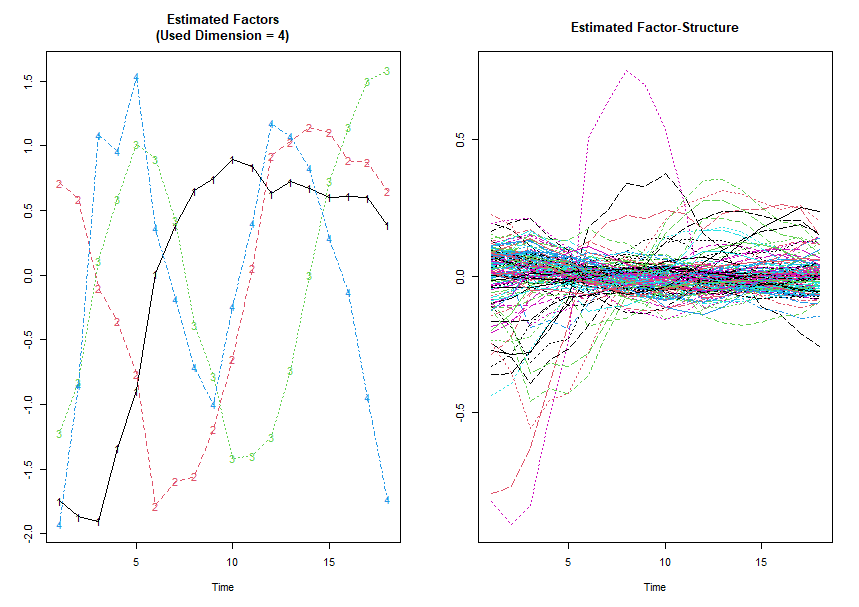
\includegraphics[width=\textwidth]{Images/eup_factors_reduced.png}
  \label{fig:image1}
\end{figure}


\subsection{Robustness}

\subsubsection{Boostrap-Regression Analysis}

While the estimation procedure in \Cref{main_estimates} accounts for serial correlation and heteroskedasticity in the time dimension, it may not fully capture all the intricacies of the underlying data-generating process. To address any residual concerns related to misspecification I run a country-level clustered non-parametric bootstrap regression analysis, focusing on the preferred specification with $P = 4$ lagged regressors. This method produces cluster-robust standard errors, enhancing the precision of the analysis. For the bootstrap exercise, I set the number of replications to $10,000$. The estimation of factor dimension is done through the PC1 criterion across all replications. 

\Cref{eup_results_boostrap} displays the results of the bootstrap-regression analysis for the democracy variable, while \Cref{fig:image2} displays the histogram plot and smoothed density for the bootstrap coefficients for democracy.  The full results of the exercise can be viewed in \Cref{eup_apendix}.  Reassuringly, the bootstrap standard errors are of the same order of magnitude and indeed quite close to the ones shown in \Cref{eup_results}. Further, the median of the bootstrap coefficients for the democracy variable lies quite close to the original estimates in the same table.
This speaks for the robustness of the specification used in \Cref{main_estimates}. 


The computed 95\% \ac{CI} —encompassing normal, percentile, and bias-corrected and accelerated (BCa) approaches— for the democracy measure collectively encapsulate 0. This indicates that the effect of democracy on GDP is not statistically singificant at the $5\%$ level. 


\begin{table}[htb]
\caption{Effect of Democracy on GDP per capita growth: \\
(\ac{Eup} method, Bootstrap-Regression Analysis)}
\label{eup_results_boostrap}
\small
\centering
\begin{tabular}{cc}
\hline
Statistic & Democracy \\
\hline 
Original Estimate & -0.0020 \\
Bias & 0.0008 \\
Bootstrap Standard Error & 0.0046 \\
Normal 95\% CI & (-0.0118, 0.0062) \\
Percentile 95\% CI & (-0.0107, 0.0074) \\
BCa 95\% CI & (-0.0127, 0.0056) \\
\hline
\end{tabular}
\end{table}


\begin{figure}[htb]
  \caption{Histogram and Density Plot of Bootstrap Regression Coefficients for Democracy \\
  (\ac{Eup} method)}
  \centering
  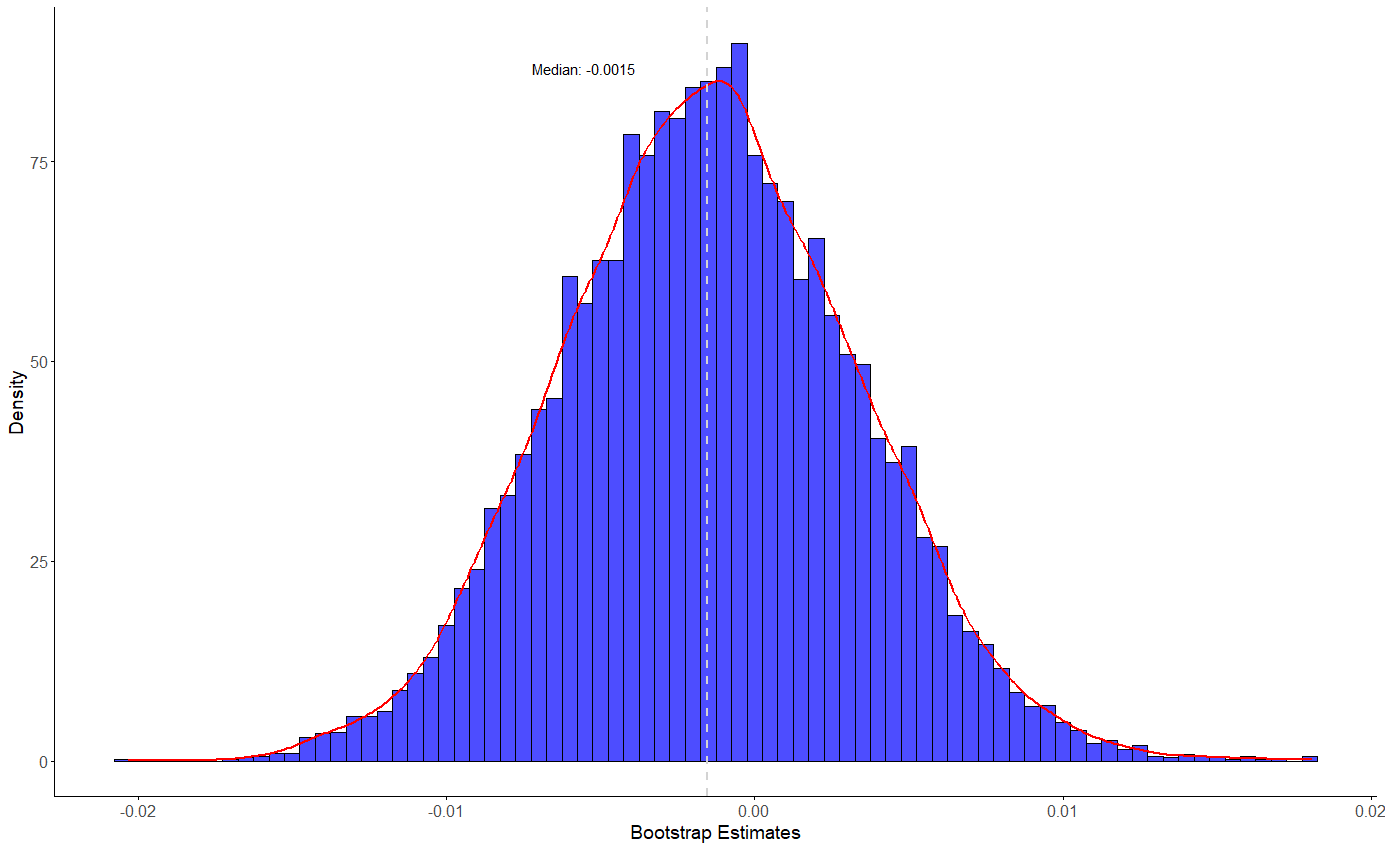
\includegraphics[width=\textwidth]{Images/hist_eup.png}
  \label{fig:image2}
\end{figure}


\subsubsection{Size of the Democracy Coefficient}

The results presented above provide evidence that the effect of democracy on \ac{GDP} growth is notably small and  non-significant. Though the lack of statistical significance might suggest that this effect is negligible, further investigation is warranted. Specifically, it is of particular interest to determine if the observed coefficient is sufficiently small to render its impact on growth inconsequential for practical purposes.

I investigate this issue by conducting a one-sided hypothesis test. The objective is to determine whether the observed coefficient falls significantly below a threshold set at $25 \%$ of the estimated coefficient in column (iv) of \Cref{within_results_diff}. Formally, the null and alternative hypotheses can be written as:
\begin{align*}
H_0 &: \beta \geq \beta_U \\
H_1 &: \beta < \beta_U
\end{align*}
With $\beta_U = \frac{1}{4} \times 0.0172 \approx 0.0043$. The results of the one-sided test are shown in \Cref{tab:test}. I reject the null hypothesis at the $5\%$ significance level that the effect of democracy on growth is at least $\beta_U$. This provides further evidence that once the unobserved factor structure is explicitly accounted for in the estimation procedure, the effect of democracy on growth is substantially diminished and potentially less influential than previously believed.

\begin{table}[htb]
    \caption{One-sided Hypothesis Test Results for the Effect of Democracy on GDP Growth \\
    (\ac{Eup} Method)}\label{tab:test}
    \centering
    \begin{tabular}{cc}
        \hline
        Statistic & Original Specification  \\
        \hline
        Coefficient Estimate & $-0.0020$\\
        Standard Error & 0.0036 \\
        $z$-value & $-1.77565$ \\
        $p$-value & 0.0379 \\
        $\text{OSCI}_{95}$  for $\beta$ & $]-\infty, 0.0038]$ \\
        \hline
    \end{tabular}

    \label{tab:results}
\end{table}


\section{Conclusion}

In this dissertation, I provide a comparative study of the methods proposed by \citet{bai2009panel}, \citet{kneip2012new} and \citet{bada2012phtt}. The theoretical underpinnings of the considered estimations are discussed thoroughly, and Monte Carlo simulations provide new insights into the finite sample performance of the estimators under varying conditions. The \ac{Eup} estimator emerges as the preferred approach and shows a good performance overall. In contrast, the \ac{KSS} estimator produces mixed results, as the method performs poorly whenever the unknown factors aren't smooth. As expected, the effectiveness of the method advanced by \citet{bai2009panel} relies on accurately estimating the factor dimension externally. Additionally, the results indicate that explicitly modeling the factor structure can mitigate inefficiencies otherwise introduced by including autocorrelated error terms. 

One of this dissertation's key contributions lies in its application of factor-based methods to study the relationship between democracy and \ac{GDP} growth. By revisiting the findings of \citet{acemoglu2019democracy} and \citet{chen2019mastering} through the estimators studied through this work,  I show the explicit modeling of the unobserved factor structure reveals a small and statistically insignificant effect of democracy on \ac{GDP} growth. This warrants a further discussion of the issue and draws attention to the validity of the assumption of previous studies. 

In summation, this work underscores the importance of factor-based estimation strategies in enhancing the precision and reliability of econometric analyses in the presence of unobserved heterogeneity. Further developments in this direction could help disentangle and solve previously obscured relationships, offering clearer insights into the nuanced dynamics of socio-economic phenomena.



\clearpage


\addcontentsline{toc}{section}{References}
\thispagestyle{plainfancy}
\bibliography{bibliograpy.bib}


\begin{appendix}
\addcontentsline{toc}{section}{Appendices}
    %\pagenumbering{roman}
    \setcounter{table}{0}
\renewcommand{\thetable}{A\arabic{table}}

\section{Monte Carlo Simulation Results}\label{monte_carlo_appendix}
\thispagestyle{plainfancy}
\setlength\tabcolsep{3.4pt}

\subsection{Homoskedastic Errors with Exogenous Regressors}\label{homo_sim_results}
\begin{table}[b!]
\caption{Monte Carlo simulation results for \ac{DGP}1}\label{DGP1}
    \small
    \centering
 \begin{tabular}{lcccccc} 
\hline \multicolumn{6}{c}{MSE of Effects} \\ \hline 
$n$ & $T$ & KSS & Eup & $d_{KSS}$ & $d_{Eup}$ \\
\hline
30 & 12 &  0.7285  &  1.0413  &  2.0000  &  2.9390  \\
& 30 &  0.2749  &  0.3980  &  2.0310  &  2.4350  \\
100 & 12 &  0.3807  &  0.4259  &  2.0000  &  2.4810  \\
& 30 &  0.1754  &  0.1931  &  2.0030  &  2.2190  \\
300 & 12 &  0.2873  &  0.2912  &  2.0000  &  2.2240  \\
& 30 &  0.1484  &  0.1454  &  2.0060  &  2.2420  \\
\end{tabular} 
\begin{tabular}{ccccccc} 
\hline 
\multicolumn{7}{c}{MSE, Bias, Variance for Coefficients} \\ \hline 
& \multicolumn{3}{c}{$T=12$} & \multicolumn{3}{c}{$T=30$} \\ \cline{2-4} \cline{5-7} 
& KSS & Eup & Within & KSS & Eup & Within \\\multicolumn{7}{l}{$n = 30 } \\MSE  & 0.00395 & 0.00509 & 0.02882 & 0.00113 & 0.00141 & 0.01038\\ BIAS1  & -0.00383 & -0.00605 & -0.0097 & 0.0010 & 0.00067 & -0.00041\\ BIAS2  & -0.00107 & -0.00202 & 0.00430 & -0.00088 & -0.00099 & 0.00297\\ VAR1  & 0.06637 & 0.06303 & 0.13016 & 0.03642 & 0.03414 & 0.07439\\ VAR2  & 0.06636 & 0.06304 & 0.13008 & 0.03638 & 0.03410 & 0.07427\\ \hline 
\multicolumn{7}{l}{$n = 100 } \\MSE  & 0.00120 & 0.00127 & 0.01060 & 0.00036 & 4e-04 & 0.00400\\ BIAS1  & -0.00202 & -0.00119 & -0.00216 & 0.00063 & 0.00098 & 0.00174\\ BIAS2  & 0.00011 & 0.00064 & 0.00054 & 0.00063 & 0.00088 & 0.00121\\ VAR1  & 0.03521 & 0.03394 & 0.07055 & 0.01942 & 0.01860 & 0.04063\\ VAR2  & 0.03526 & 0.03398 & 0.07056 & 0.01941 & 0.01860 & 0.04062\\ \hline 
\multicolumn{7}{l}{$n = 300 } \\MSE  & 0.00039 & 0.00043 & 0.00337 & 0.00012 & 0.00012 & 0.00105\\ BIAS1  & -0.00109 & -0.00083 & 0.00169 & -7e-05 & -5e-05 & -0.00258\\ BIAS2  & 0.00016 & 0.00022 & -0.00129 & -0.00025 & -7e-05 & 0.00119\\ VAR1  & 0.02030 & 0.01949 & 0.04143 & 0.01118 & 0.01078 & 0.02374\\ VAR2  & 0.02031 & 0.01949 & 0.04142 & 0.01117 & 0.01079 & 0.02374\\ \hline 
\end{tabular} 

\end{table}

\begin{table}[b]
\caption{Monte Carlo simulation results for \ac{DGP}2} \label{DGP2}
      \small
    \centering
 \begin{tabular}{lccccccc} 
\hline \multicolumn{7}{c}{MSE of Effects} \\ \hline 
$n$ & $T$ & KSS & Bai & Eup & $d_{KSS}$ & $d_{Bai}$ & $d_{Eup}$ \\
\hline
30 & 12 &  34.6197  &  5.1895  &  0.5866  &  1.1690  &  8.0000  &  2.5970  \\
& 30 &  18.7861  &  1.6238  &  0.0748  &  1.0890  &  8.0000  &  1.0230  \\
100 & 12 &  21.1234  &  1.4683  &  0.0968  &  1.0380  &  8.0000  &  1.0060  \\
& 30 &  12.8899  &  0.4892  &  0.0433  &  1.0080  &  8.0000  &  1.0000  \\
300 & 12 &  17.9368  &  0.9283  &  0.0868  &  1.0020  &  8.0000  &  1.0000  \\
& 30 &  11.7004  &  0.3731  &  0.0370  &  1.0020  &  8.0000  &  1.0000  \\
\end{tabular} 
\begin{tabular}{ccccccccc} 
\hline 
\multicolumn{9}{c}{MSE, Bias, Variance for Coefficients} \\ \hline 
& \multicolumn{4}{c}{$T=12$} & \multicolumn{4}{c}{$T=30$} \\ \cline{2-5} \cline{6-9} 
& KSS &  Bai & Eup & Within & KSS & Bai &  Eup & Within \\\multicolumn{8}{l}{$n = 30 } \\MSE  & 0.14589 & 0.03000 & 0.00309 & 0.86332 & 0.07331 & 0.00579 & 0.00061 & 0.80906\\ BIAS1  & 0.01399 & -0.00079 & -0.0011 & 0.00225 & -0.00538 & -0.00533 & -0.00026 & 0.00223\\ BIAS2  & -0.00896 & 0.00269 & 0.00104 & 0.02220 & -0.00516 & -0.00295 & 0.00085 & 0.03484\\ VAR1  & 0.29724 & 0.12825 & 0.04154 & 0.64902 & 0.16870 & 0.03026 & 0.02340 & 0.59364\\ VAR2  & 0.29713 & 0.12781 & 0.04158 & 0.64840 & 0.16869 & 0.03022 & 0.02339 & 0.59210\\ \hline 
\multicolumn{8}{l}{$n = 100 } \\MSE  & 0.04493 & 0.00463 & 0.00045 & 0.25214 & 0.02080 & 4e-04 & 0.00015 & 0.30042\\ BIAS1  & -0.00784 & 0.00116 & 0.00023 & -0.00488 & 0.00161 & 0.00089 & -2e-04 & -0.00174\\ BIAS2  & -0.00420 & -0.00362 & 0.00027 & 0.00933 & 0.00022 & -0.00035 & 0.00014 & -0.00228\\ VAR1  & 0.15368 & 0.03662 & 0.02059 & 0.34846 & 0.08608 & 0.01391 & 0.01263 & 0.32538\\ VAR2  & 0.15356 & 0.03666 & 0.02059 & 0.34845 & 0.08606 & 0.01391 & 0.01262 & 0.32514\\ \hline 
\multicolumn{8}{l}{$n = 300 } \\MSE  & 0.01424 & 0.00135 & 0.00015 & 0.08404 & 0.00657 & 9e-05 & 5e-05 & 0.08561\\ BIAS1  & 0.00135 & 0.00158 & 0.00024 & -0.00436 & -0.00388 & -0.00034 & -0.00026 & 0.00092\\ BIAS2  & 0.00578 & -0.00037 & -0.00033 & -0.01926 & 0.00169 & 0.00037 & 5e-04 & -0.01251\\ VAR1  & 0.08518 & 0.01979 & 0.01182 & 0.20363 & 0.04741 & 0.00797 & 0.00726 & 0.19078\\ VAR2  & 0.08526 & 0.01982 & 0.01183 & 0.20366 & 0.04743 & 0.00797 & 0.00726 & 0.19081\\ \hline 
\end{tabular} 

\end{table}

\begin{table}[htb]
\caption{Monte Carlo simulation results for \ac{DGP}3}\label{DGP3}
      \small
    \centering
 \begin{tabular}{lcccccc} 
\hline \multicolumn{6}{c}{MSE of Effects} \\ \hline 
$n$ & $T$ & KSS & Eup & $d_{KSS}$ & $d_{Eup}$ \\
\hline
30 & 12 &  1.4970  &  0.3913  &  2.6210  &  2.8830  \\
& 30 &  11.2204  &  0.1355  &  0.6010  &  2.0380  \\
100 & 12 &  0.5072  &  0.1895  &  2.4440  &  2.0310  \\
& 30 &  9.4474  &  0.0855  &  0.3440  &  2.0000  \\
300 & 12 &  0.3032  &  0.1728  &  2.2920  &  2.0000  \\
& 30 &  9.0916  &  0.0732  &  0.1000  &  2.0000  \\
\end{tabular} 
\begin{tabular}{ccccccc} 
\hline 
\multicolumn{7}{c}{MSE, Bias, Variance for Coefficients} \\ \hline 
& \multicolumn{3}{c}{$T=12$} & \multicolumn{3}{c}{$T=30$} \\ \cline{2-4} \cline{5-7} 
& KSS & Eup & Within & KSS & Eup & Within \\\multicolumn{7}{l}{$n = 30 } \\MSE  & 0.00976 & 0.00227 & 0.04683 & 0.01711 & 0.00059 & 0.01575\\ BIAS1  & -0.00549 & -0.00149 & 0.00992 & -0.00299 & -6e-05 & -0.00285\\ BIAS2  & -0.00303 & 0.00064 & -0.00404 & 0.00182 & -0.00011 & 0.00175\\ VAR1  & 0.09323 & 0.04106 & 0.17103 & 0.09263 & 0.02373 & 0.10165\\ VAR2  & 0.09308 & 0.04105 & 0.17108 & 0.09260 & 0.02374 & 0.10166\\ \hline 
\multicolumn{7}{l}{$n = 100 } \\MSE  & 0.00265 & 0.00048 & 0.01203 & 0.00424 & 0.00017 & 0.00422\\ BIAS1  & 0.0014 & 0.00018 & 0.00261 & 0.00016 & 0.00023 & -0.00051\\ BIAS2  & 0.00134 & -4e-04 & 0.00299 & 0.00037 & -0.00019 & -0.00016\\ VAR1  & 0.04930 & 0.02112 & 0.09308 & 0.04502 & 0.01265 & 0.05495\\ VAR2  & 0.04927 & 0.02113 & 0.09295 & 0.04505 & 0.01265 & 0.05497\\ \hline 
\multicolumn{7}{l}{$n = 300 } \\MSE  & 0.00100 & 0.00016 & 0.00451 & 0.00096 & 5e-05 & 0.00134\\ BIAS1  & 0.00231 & -0.00095 & 0.00208 & 0.00087 & -0.00041 & 0.00084\\ BIAS2  & 0.00033 & 0.00085 & 0.00158 & -0.00232 & 0.00036 & -0.00282\\ VAR1  & 0.02838 & 0.01209 & 0.05424 & 0.02328 & 0.00725 & 0.03216\\ VAR2  & 0.02842 & 0.01208 & 0.05428 & 0.02329 & 0.00725 & 0.03216\\ \hline 
\end{tabular} 

\end{table}

\begin{table}[htb]
\caption{Monte Carlo simulation results for \ac{DGP}4}\label{DGP4}
      \small
    \centering
 \begin{tabular}{lccccccccc} 
\hline \multicolumn{8}{c}{MSE of the Time-Varying Individual Effects} \\ \hline 
$n$ & $T$ & KSS & $ \text{Bai}_{\hat{d} = 8}$ & $\text{Bai}_{\hat{d} = d}$ & Eup & $\hat{d}_{KSS}$ & $\hat{d}_{Eup}$ \\
\hline
30 & 12 &  0.5544  &  1.5392  &  0.6144  &  1.0360  &  1.0000  &  2.5890  \\
& 30 &  0.1573  &  0.9380  &  0.2299  &  0.2351  &  1.0000  &  1.0090  \\
100 & 12 &  0.2017  &  0.9803  &  0.1938  &  0.1979  &  1.0000  &  1.0070  \\
& 30 &  0.0723  &  0.5173  &  0.0799  &  0.0805  &  1.0000  &  1.0000  \\
300 & 12 &  0.1277  &  0.7990  &  0.1202  &  0.1213  &  1.0000  &  1.0000  \\
& 30 &  0.0464  &  0.3890  &  0.0485  &  0.0488  &  1.0000  &  1.0000  \\
\end{tabular} 
\begin{tabular}{ccccccccccc} 
\hline 
\multicolumn{10}{c}{MSE, Bias, Variance and Power for the Common Slope Coefficients} \\ \hline 
& \multicolumn{5}{c}{$T=12$} & \multicolumn{5}{c}{$T=30$} \\ \cline{2-6} \cline{7-11} 
& KSS & $ \text{Bai}_{\hat{d} = 8}$ & $\text{Bai}_{\hat{d} = d}$& Eup & Within & KSS & \text{Bai}_{\hat{d} = 8} & \text{Bai}_{\hat{d} = d} & Eup & Within \\\multicolumn{8}{l}{$n = 30 } \\$\text{MSE}_\hat{\beta}$ & 0.0037 & 0.0126 & 0.0035 & 0.0049 & 0.0030 & 0.0010 & 0.0025 & 0.0012 & 0.0012 & 0.0010\\Bias $\hat{\beta}_1$ & -0.0021 & -0.0032 & 0.0003 & -0.0007 & -0.0018 & 0.0000 & 0.0002 & 0.0000 & 0.0000 & 0.0002\\Bias $\hat{\beta}_2$ & 0.0021 & 0.0029 & 0.0032 & 0.0012 & 0.0021 & 0.0007 & 0.0005 & 0.0007 & 0.0008 & 0.0008\\$\text{Var}(\hat{\beta}_1)$ & 0.0604 & 0.1343 & 0.0503 & 0.0524 & 0.0535 & 0.0337 & 0.0348 & 0.0301 & 0.0301 & 0.0318\\$\text{Var}(\hat{\beta}_2)$ & 0.0603 & 0.1343 & 0.0503 & 0.0524 & 0.0534 & 0.0337 & 0.0348 & 0.0301 & 0.0301 & 0.0318\\Power $\hat{\beta}_1$ & 1.0000 & 0.9710 & 1.0000 & 1.0000 & 1.0000 & 1.0000 & 1.0000 & 1.0000 & 1.0000 & 1.0000\\Power $\hat{\beta}_2$ & 1.0000 & 0.9730 & 1.0000 & 1.0000 & 1.0000 & 1.0000 & 1.0000 & 1.0000 & 1.0000 & 1.0000\\ \hline 
\multicolumn{8}{l}{$n = 100 } \\$\text{MSE}_\hat{\beta}$ & 0.0011 & 0.0027 & 0.0009 & 0.0009 & 0.0009 & 0.0003 & 0.0005 & 0.0003 & 0.0003 & 0.0003\\Bias $\hat{\beta}_1$ & 0.0005 & -0.0003 & -0.0006 & -0.0006 & -0.0001 & 0.0003 & 0.0004 & 0.0002 & 0.0002 & 0.0003\\Bias $\hat{\beta}_2$ & 0.0014 & -0.0014 & 0.0003 & 0.0002 & 0.0008 & -0.0001 & 0.0004 & -0.0001 & -0.0001 & -0.0001\\$\text{Var}(\hat{\beta}_1)$ & 0.0324 & 0.0446 & 0.0283 & 0.0283 & 0.0289 & 0.0181 & 0.0183 & 0.0169 & 0.0169 & 0.0172\\$\text{Var}(\hat{\beta}_2)$ & 0.0324 & 0.0447 & 0.0283 & 0.0283 & 0.0289 & 0.0181 & 0.0183 & 0.0169 & 0.0169 & 0.0172\\Power $\hat{\beta}_1$ & 1.0000 & 1.0000 & 1.0000 & 1.0000 & 1.0000 & 1.0000 & 1.0000 & 1.0000 & 1.0000 & 1.0000\\Power $\hat{\beta}_2$ & 1.0000 & 1.0000 & 1.0000 & 1.0000 & 1.0000 & 1.0000 & 1.0000 & 1.0000 & 1.0000 & 1.0000\\ \hline 
\multicolumn{8}{l}{$n = 300 } \\$\text{MSE}_\hat{\beta}$ & 0.0004 & 0.0008 & 0.0003 & 0.0003 & 0.0003 & 0.0001 & 0.0002 & 0.0001 & 0.0001 & 0.0001\\Bias $\hat{\beta}_1$ & -0.0008 & -0.0031 & -0.0007 & -0.0007 & -0.0007 & 0.0004 & 0.0006 & 0.0005 & 0.0005 & 0.0005\\Bias $\hat{\beta}_2$ & 0.0025 & 0.0042 & 0.0023 & 0.0023 & 0.0021 & 0.0002 & 0.0012 & 0.0004 & 0.0004 & 0.0004\\$\text{Var}(\hat{\beta}_1)$ & 0.0187 & 0.0261 & 0.0167 & 0.0167 & 0.0168 & 0.0105 & 0.0109 & 0.0100 & 0.0100 & 0.0100\\$\text{Var}(\hat{\beta}_2)$ & 0.0187 & 0.0261 & 0.0167 & 0.0167 & 0.0169 & 0.0104 & 0.0109 & 0.0099 & 0.0099 & 0.0100\\Power $\hat{\beta}_1$ & 1.0000 & 1.0000 & 1.0000 & 1.0000 & 1.0000 & 1.0000 & 1.0000 & 1.0000 & 1.0000 & 1.0000\\Power $\hat{\beta}_2$ & 1.0000 & 1.0000 & 1.0000 & 1.0000 & 1.0000 & 1.0000 & 1.0000 & 1.0000 & 1.0000 & 1.0000\\ \hline 
\end{tabular} 

\end{table}

\clearpage

\subsubsection{Homoskedastic Errors with Exogenous Regressors, \acs{KSS} Approach with Known Dimension}\label{exercise_sim}

\begin{table}[htb]
\caption{Monte Carlo simulation results for \ac{DGP}3}
     \small
    \centering
 \begin{tabular}{lccccccccc} 
\hline \multicolumn{8}{c}{MSE of the Time-Varying Individual Effects} \\ \hline 
$n$ & $T$ & KSS & $ \text{Bai}_{\hat{d} = 8}$ & $\text{Bai}_{\hat{d} = d}$ & Eup & $\hat{d}_{KSS}$ & $\hat{d}_{Eup}$ \\
\hline
30 & 12 &  1.1096  &  1.0137  &  0.2287  &  0.3999  &  2.0000  &  2.8800  \\
& 30 &  10.7594  &  0.6389  &  0.1323  &  0.1379  &  2.0000  &  2.0340  \\
100 & 12 &  0.2817  &  0.8041  &  0.1845  &  0.1905  &  2.0000  &  2.0310  \\
& 30 &  9.5008  &  0.4439  &  0.0858  &  0.0858  &  2.0000  &  2.0000  \\
300 & 12 &  0.1989  &  0.7345  &  0.1730  &  0.1730  &  2.0000  &  2.0000  \\
& 30 &  9.1382  &  0.3624  &  0.0732  &  0.0732  &  2.0000  &  2.0000  \\
\end{tabular} 
\begin{tabular}{ccccccccccc} 
\hline 
\multicolumn{10}{c}{MSE, Bias, Variance and Power for the Common Slope Coefficients} \\ \hline 
& \multicolumn{5}{c}{$T=12$} & \multicolumn{5}{c}{$T=30$} \\ \cline{2-6} \cline{7-11} 
& KSS & $ \text{Bai}_{\hat{d} = 8}$ & $\text{Bai}_{\hat{d} = d}$& Eup & Within & KSS & \text{Bai}_{\hat{d} = 8} & \text{Bai}_{\hat{d} = d} & Eup & Within \\\multicolumn{8}{l}{$n = 30 } \\$\text{MSE}_\hat{\beta}$ & 0.0090 & 0.0100 & 0.0017 & 0.0022 & 0.0469 & 0.0149 & 0.0014 & 0.0006 & 0.0006 & 0.0130\\Bias $\hat{\beta}_1$ & 0.0076 & -0.0019 & 0.0014 & 0.0006 & -0.0040 & 0.0000 & -0.0023 & -0.0014 & -0.0014 & 0.0001\\Bias $\hat{\beta}_2$ & 0.0042 & -0.0009 & -0.0017 & -0.0018 & 0.0074 & 0.0055 & 0.0009 & 0.0013 & 0.0012 & 0.0047\\$\text{Var}(\hat{\beta}_1)$ & 0.1212 & 0.1062 & 0.0399 & 0.0411 & 0.1713 & 0.1110 & 0.0272 & 0.0238 & 0.0238 & 0.1017\\$\text{Var}(\hat{\beta}_2)$ & 0.1214 & 0.1057 & 0.0399 & 0.0411 & 0.1717 & 0.1109 & 0.0272 & 0.0238 & 0.0238 & 0.1017\\Power $\hat{\beta}_1$ & 0.9730 & 0.9860 & 1.0000 & 1.0000 & 0.7670 & 0.9850 & 1.0000 & 1.0000 & 1.0000 & 0.9950\\Power $\hat{\beta}_2$ & 0.9720 & 0.9890 & 1.0000 & 1.0000 & 0.7840 & 0.9860 & 1.0000 & 1.0000 & 1.0000 & 0.9930\\ \hline 
\multicolumn{8}{l}{$n = 100 } \\$\text{MSE}_\hat{\beta}$ & 0.0026 & 0.0018 & 0.0005 & 0.0005 & 0.0134 & 0.0051 & 0.0003 & 0.0002 & 0.0002 & 0.0043\\Bias $\hat{\beta}_1$ & 0.0004 & -0.0012 & -0.0005 & -0.0007 & -0.0011 & -0.0003 & -0.0002 & 0.0000 & 0.0000 & -0.0002\\Bias $\hat{\beta}_2$ & 0.0001 & 0.0000 & 0.0003 & 0.0003 & 0.0029 & 0.0019 & 0.0003 & 0.0001 & 0.0001 & 0.0012\\$\text{Var}(\hat{\beta}_1)$ & 0.0553 & 0.0327 & 0.0211 & 0.0211 & 0.0924 & 0.0588 & 0.0136 & 0.0127 & 0.0127 & 0.0550\\$\text{Var}(\hat{\beta}_2)$ & 0.0554 & 0.0328 & 0.0211 & 0.0211 & 0.0925 & 0.0588 & 0.0136 & 0.0127 & 0.0127 & 0.0550\\Power $\hat{\beta}_1$ & 1.0000 & 1.0000 & 1.0000 & 1.0000 & 0.9920 & 1.0000 & 1.0000 & 1.0000 & 1.0000 & 1.0000\\Power $\hat{\beta}_2$ & 1.0000 & 1.0000 & 1.0000 & 1.0000 & 0.9990 & 1.0000 & 1.0000 & 1.0000 & 1.0000 & 1.0000\\ \hline 
\multicolumn{8}{l}{$n = 300 } \\$\text{MSE}_\hat{\beta}$ & 0.0009 & 0.0005 & 0.0002 & 0.0002 & 0.0042 & 0.0017 & 0.0001 & 0.0001 & 0.0001 & 0.0015\\Bias $\hat{\beta}_1$ & 0.0006 & 0.0003 & -0.0004 & -0.0004 & 0.0001 & 0.0001 & -0.0006 & -0.0003 & -0.0003 & 0.0000\\Bias $\hat{\beta}_2$ & 0.0023 & -0.0002 & 0.0004 & 0.0004 & 0.0028 & -0.0017 & 0.0006 & 0.0003 & 0.0003 & -0.0016\\$\text{Var}(\hat{\beta}_1)$ & 0.0294 & 0.0182 & 0.0121 & 0.0121 & 0.0543 & 0.0339 & 0.0079 & 0.0073 & 0.0073 & 0.0322\\$\text{Var}(\hat{\beta}_2)$ & 0.0294 & 0.0182 & 0.0121 & 0.0121 & 0.0543 & 0.0339 & 0.0079 & 0.0073 & 0.0073 & 0.0322\\Power $\hat{\beta}_1$ & 1.0000 & 1.0000 & 1.0000 & 1.0000 & 1.0000 & 1.0000 & 1.0000 & 1.0000 & 1.0000 & 1.0000\\Power $\hat{\beta}_2$ & 1.0000 & 1.0000 & 1.0000 & 1.0000 & 1.0000 & 1.0000 & 1.0000 & 1.0000 & 1.0000 & 1.0000\\ \hline 
\end{tabular} 

\end{table}

\clearpage

\subsection{Homoskedastic Error Terms with Endogenous Regressors}\label{endo_sim}

\begin{table}[htb]
\caption{Monte Carlo simulation results for \ac{DGP}1}
    \small
    \centering
 \begin{tabular}{lccccccc} 
\hline \multicolumn{7}{c}{MSE of Effects} \\ \hline 
$n$ & $T$ & KSS & Bai & Eup & $d_{KSS}$ & $d_{Bai}$ & $d_{Eup}$ \\
\hline
30 & 12 &  0.4653  &  1.3425  &  0.7329  &  2.0010  &  6.0000  &  2.9200  \\
& 30 &  0.2044  &  0.3017  &  0.2971  &  2.0210  &  2.4620  &  2.4230  \\
100 & 12 &  0.3115  &  0.7605  &  0.3580  &  2.0000  &  5.9230  &  2.4830  \\
& 30 &  0.1548  &  0.1693  &  0.1693  &  2.0080  &  2.2520  &  2.2520  \\
300 & 12 &  0.2613  &  0.3902  &  0.2657  &  2.0000  &  3.5560  &  2.2200  \\
& 30 &  0.1412  &  0.1374  &  0.1374  &  2.0060  &  2.2620  &  2.2620  \\
\end{tabular} 
\begin{tabular}{cccccccc} 
\hline 
\multicolumn{8}{c}{MSE, Bias, Variance for Coefficients} \\ \hline 
& \multicolumn{4}{c}{$T=12$} & \multicolumn{4}{c}{$T=30$} \\ \cline{2-5} \cline{6-9} 
& KSS &  Bai & Eup & Within & KSS & Bai &  Eup & Within \\\multicolumn{8}{l}{$n = 30 } \\MSE  & 0.00374 & 0.00973 & 0.00542 & 0.03051 & 0.00118 & 0.00146 & 0.00144 & 0.01066\\ BIAS1  & -3e-05 & -2e-04 & -2e-04 & 0.00553 & 0.00241 & 0.00244 & 0.00252 & -0.00271\\ BIAS2  & 1e-04 & 7e-05 & 4e-05 & 0.00844 & 7e-05 & 1e-04 & 1e-04 & 0.00811\\ VAR1  & 0.06654 & 0.07987 & 0.06258 & 0.12851 & 0.03646 & 0.03401 & 0.03400 & 0.07434\\ VAR2  & 0.00120 & 0.00151 & 0.00119 & 0.00242 & 0.00071 & 7e-04 & 7e-04 & 0.00147\\ POWER1  & 1.00000 & 0.99900 & 1.00000 & 0.92000 & 1.00000 & 1.00000 & 1.00000 & 1.00000\\ POWER2  & 1.00000 & 1.00000 & 1.00000 & 1.00000 & 1.00000 & 1.00000 & 1.00000 & 1.00000\\ \hline 
\multicolumn{8}{l}{$n = 100 } \\MSE  & 0.00122 & 0.00240 & 0.00139 & 0.00848 & 0.00035 & 4e-04 & 4e-04 & 0.00379\\ BIAS1  & -0.00074 & -0.00043 & -0.00056 & 0.00096 & -0.00031 & -3e-04 & -3e-04 & -0.00096\\ BIAS2  & 0.00012 & 1e-05 & 7e-05 & 0.00816 & 7e-05 & 1e-04 & 1e-04 & 0.00763\\ VAR1  & 0.03528 & 0.04114 & 0.03396 & 0.06952 & 0.01943 & 0.01859 & 0.01859 & 0.03989\\ VAR2  & 0.00063 & 0.00073 & 0.00061 & 0.00131 & 0.00037 & 0.00037 & 0.00037 & 0.00079\\ POWER1  & 1.00000 & 1.00000 & 1.00000 & 1.00000 & 1.00000 & 1.00000 & 1.00000 & 1.00000\\ POWER2  & 1.00000 & 1.00000 & 1.00000 & 1.00000 & 1.00000 & 1.00000 & 1.00000 & 1.00000\\ \hline 
\multicolumn{8}{l}{$n = 300 } \\MSE  & 0.00042 & 0.00057 & 0.00043 & 0.00283 & 0.00011 & 0.00012 & 0.00012 & 0.00108\\ BIAS1  & -4e-05 & -0.00055 & -0.00073 & -0.00049 & -5e-05 & 5e-05 & 6e-05 & -0.00094\\ BIAS2  & 0.00013 & 1e-04 & 0.00011 & 0.00805 & 5e-05 & 8e-05 & 8e-05 & 0.00755\\ VAR1  & 0.02033 & 0.02117 & 0.01951 & 0.04080 & 0.01118 & 0.01079 & 0.01079 & 0.02333\\ VAR2  & 0.00035 & 0.00037 & 0.00035 & 0.00075 & 0.00021 & 0.00021 & 0.00021 & 0.00045\\ POWER1  & 1.00000 & 1.00000 & 1.00000 & 1.00000 & 1.00000 & 1.00000 & 1.00000 & 1.00000\\ POWER2  & 1.00000 & 1.00000 & 1.00000 & 1.00000 & 1.00000 & 1.00000 & 1.00000 & 1.00000\\ \hline 
\end{tabular} 

\end{table}
    
\begin{table}[htb]
\caption{Monte Carlo simulation results for \ac{DGP}2}
      \small
    \centering
 \begin{tabular}{lcccccc} 
\hline \multicolumn{6}{c}{MSE of Effects} \\ \hline 
$n$ & $T$ & KSS & Eup & $d_{KSS}$ & $d_{Eup}$ \\
\hline
30 & 12 &  27.8636  &  0.4270  &  1.0760  &  2.5890  \\
& 30 &  14.4682  &  0.0709  &  1.0190  &  1.0110  \\
100 & 12 &  21.6325  &  0.0956  &  0.9980  &  1.0070  \\
& 30 &  13.0143  &  0.0440  &  1.0000  &  1.0000  \\
300 & 12 &  20.2115  &  0.0875  &  0.9800  &  1.0000  \\
& 30 &  11.1849  &  0.0370  &  1.0000  &  1.0000  \\
\end{tabular} 
\begin{tabular}{ccccccc} 
\hline 
\multicolumn{7}{c}{MSE, Bias, Variance for Coefficients} \\ \hline 
& \multicolumn{3}{c}{$T=12$} & \multicolumn{3}{c}{$T=30$} \\ \cline{2-4} \cline{5-7} 
& KSS & Eup & Within & KSS & Eup & Within \\\multicolumn{7}{l}{$n = 30 } \\MSE  & 0.15394 & 0.00068 & 0.78237 & 0.06309 & 8e-05 & 0.73332\\ BIAS1  & -0.00206 & 0.00034 & 0.04591 & -0.00264 & -0.00055 & 0.03764\\ BIAS2  & 0.01110 & -2e-05 & 0.02954 & 0.00447 & 0.00000 & 0.02722\\ VAR1  & 0.29694 & 0.01295 & 0.59034 & 0.16286 & 0.00721 & 0.55882\\ VAR2  & 0.00207 & 0.00045 & 0.00375 & 7e-04 & 0.00017 & 0.00222\\ \hline 
\multicolumn{7}{l}{$n = 100 } \\MSE  & 0.04510 & 5e-05 & 0.21313 & 0.01858 & 2e-05 & 0.19168\\ BIAS1  & -0.01657 & 5e-05 & -0.00568 & -0.00129 & 4e-05 & -0.01679\\ BIAS2  & 0.01016 & 0.00000 & 0.02816 & 0.00471 & 1e-05 & 0.02784\\ VAR1  & 0.15182 & 0.00619 & 0.32522 & 0.08469 & 0.00381 & 0.29101\\ VAR2  & 0.00103 & 0.00023 & 0.00200 & 0.00038 & 9e-05 & 0.00123\\ \hline 
\multicolumn{7}{l}{$n = 300 } \\MSE  & 0.01420 & 2e-05 & 0.07625 & 0.00614 & 1e-05 & 0.07306\\ BIAS1  & 0.00096 & 0.00013 & 0.01165 & -0.0082 & -9e-05 & -0.01995\\ BIAS2  & 0.01116 & -1e-05 & 0.02890 & 0.00415 & 0.00000 & 0.02770\\ VAR1  & 0.08442 & 0.00347 & 0.19062 & 0.04687 & 0.00219 & 0.17626\\ VAR2  & 6e-04 & 0.00013 & 0.00117 & 2e-04 & 5e-05 & 0.00071\\ \hline 
\end{tabular} 

\end{table}


\begin{table}[htb]
\caption{Monte Carlo simulation results for \ac{DGP}3}
      \small
    \centering
 \begin{tabular}{lccccccccc} 
\hline \multicolumn{8}{c}{MSE of the Time-Varying Individual Effects} \\ \hline 
$n$ & $T$ & KSS & $ \text{Bai}_{\hat{d} = 8}$ & $\text{Bai}_{\hat{d} = d}$ & Eup & $\hat{d}_{KSS}$ & $\hat{d}_{Eup}$ \\
\hline
30 & 12 &  0.7776  &  0.9903  &  0.2281  &  0.3854  &  2.4720  &  2.8780  \\
& 30 &  9.9400  &  0.6279  &  0.1309  &  0.1351  &  0.5380  &  2.0330  \\
100 & 12 &  0.3763  &  0.8020  &  0.1849  &  0.1900  &  2.2900  &  2.0330  \\
& 30 &  9.4262  &  0.4443  &  0.0856  &  0.0856  &  0.3920  &  2.0000  \\
300 & 12 &  0.2567  &  0.7349  &  0.1739  &  0.1739  &  2.1420  &  2.0000  \\
& 30 &  9.2451  &  0.3623  &  0.0731  &  0.0731  &  0.3080  &  2.0000  \\
\end{tabular} 
\begin{tabular}{ccccccccccc} 
\hline 
\multicolumn{10}{c}{MSE, Bias, Variance and Power for the Common Slope Coefficients} \\ \hline 
& \multicolumn{5}{c}{$T=12$} & \multicolumn{5}{c}{$T=30$} \\ \cline{2-6} \cline{7-11} 
& KSS & $ \text{Bai}_{\hat{d} = 8}$ & $\text{Bai}_{\hat{d} = d}$& Eup & Within & KSS & \text{Bai}_{\hat{d} = 8} & \text{Bai}_{\hat{d} = d} & Eup & Within \\\multicolumn{8}{l}{$n = 30 } \\$\text{MSE}_\hat{\beta}$ & 0.0088 & 0.0016 & 0.0001 & 0.0001 & 0.0293 & 0.0119 & 0.0001 & 0.0000 & 0.0000 & 0.0111\\Bias $\hat{\beta}_1$ & -0.0005 & 0.0002 & -0.0001 & -0.0001 & -0.0085 & -0.0015 & -0.0002 & 0.0003 & 0.0003 & -0.0001\\Bias $\hat{\beta}_2$ & 0.0061 & 0.0005 & 0.0001 & 0.0000 & 0.0516 & 0.0510 & 0.0000 & 0.0000 & 0.0000 & 0.0511\\$\text{Var}(\hat{\beta}_1)$ & 0.0936 & 0.0324 & 0.0074 & 0.0078 & 0.1507 & 0.0564 & 0.0055 & 0.0046 & 0.0046 & 0.0892\\$\text{Var}(\hat{\beta}_2)$ & 0.0030 & 0.0057 & 0.0022 & 0.0023 & 0.0052 & 0.0032 & 0.0016 & 0.0014 & 0.0014 & 0.0032\\Power $\hat{\beta}_1$ & 1.0000 & 0.9970 & 1.0000 & 1.0000 & 0.8750 & 0.9990 & 1.0000 & 1.0000 & 1.0000 & 1.0000\\Power $\hat{\beta}_2$ & 1.0000 & 1.0000 & 1.0000 & 1.0000 & 1.0000 & 1.0000 & 1.0000 & 1.0000 & 1.0000 & 1.0000\\ \hline 
\multicolumn{8}{l}{$n = 100 } \\$\text{MSE}_\hat{\beta}$ & 0.0027 & 0.0003 & 0.0000 & 0.0000 & 0.0087 & 0.0040 & 0.0000 & 0.0000 & 0.0000 & 0.0034\\Bias $\hat{\beta}_1$ & -0.0012 & 0.0003 & 0.0004 & 0.0005 & -0.0065 & -0.0127 & 0.0000 & -0.0001 & -0.0001 & -0.0024\\Bias $\hat{\beta}_2$ & 0.0058 & -0.0001 & 0.0000 & 0.0000 & 0.0514 & 0.0507 & 0.0000 & 0.0000 & 0.0000 & 0.0511\\$\text{Var}(\hat{\beta}_1)$ & 0.0498 & 0.0076 & 0.0039 & 0.0039 & 0.0812 & 0.0240 & 0.0026 & 0.0024 & 0.0024 & 0.0484\\$\text{Var}(\hat{\beta}_2)$ & 0.0016 & 0.0018 & 0.0012 & 0.0012 & 0.0028 & 0.0017 & 0.0008 & 0.0007 & 0.0007 & 0.0017\\Power $\hat{\beta}_1$ & 1.0000 & 1.0000 & 1.0000 & 1.0000 & 1.0000 & 1.0000 & 1.0000 & 1.0000 & 1.0000 & 1.0000\\Power $\hat{\beta}_2$ & 1.0000 & 1.0000 & 1.0000 & 1.0000 & 1.0000 & 1.0000 & 1.0000 & 1.0000 & 1.0000 & 1.0000\\ \hline 
\multicolumn{8}{l}{$n = 300 } \\$\text{MSE}_\hat{\beta}$ & 0.0009 & 0.0000 & 0.0000 & 0.0000 & 0.0032 & 0.0022 & 0.0000 & 0.0000 & 0.0000 & 0.0011\\Bias $\hat{\beta}_1$ & 0.0032 & 0.0000 & 0.0000 & 0.0000 & 0.0025 & -0.0218 & 0.0000 & 0.0000 & 0.0000 & -0.0009\\Bias $\hat{\beta}_2$ & 0.0059 & 0.0000 & 0.0001 & 0.0001 & 0.0514 & 0.0505 & 0.0000 & 0.0000 & 0.0000 & 0.0511\\$\text{Var}(\hat{\beta}_1)$ & 0.0285 & 0.0039 & 0.0022 & 0.0022 & 0.0475 & 0.0118 & 0.0015 & 0.0014 & 0.0014 & 0.0283\\$\text{Var}(\hat{\beta}_2)$ & 0.0009 & 0.0010 & 0.0007 & 0.0007 & 0.0016 & 0.0010 & 0.0004 & 0.0004 & 0.0004 & 0.0010\\Power $\hat{\beta}_1$ & 1.0000 & 1.0000 & 1.0000 & 1.0000 & 1.0000 & 1.0000 & 1.0000 & 1.0000 & 1.0000 & 1.0000\\Power $\hat{\beta}_2$ & 1.0000 & 1.0000 & 1.0000 & 1.0000 & 1.0000 & 1.0000 & 1.0000 & 1.0000 & 1.0000 & 1.0000\\ \hline 
\end{tabular} 

\end{table}


\begin{table}[htb]
\caption{Monte Carlo simulation results for \ac{DGP}4}
     \small
    \centering
 \begin{tabular}{lccccccccc} 
\hline \multicolumn{8}{c}{MSE of the Time-Varying Individual Effects} \\ \hline 
$n$ & $T$ & KSS & $ \text{Bai}_{\hat{d} = 8}$ & $\text{Bai}_{\hat{d} = d}$ & Eup & $\hat{d}_{KSS}$ & $\hat{d}_{Eup}$ \\
\hline
30 & 12 &  0.2926  &  1.5161  &  0.3512  &  0.7239  &  1.0000  &  2.6300  \\
& 30 &  0.0982  &  0.8240  &  0.1404  &  0.1410  &  1.0000  &  1.0030  \\
100 & 12 &  0.1443  &  0.9603  &  0.1452  &  0.1456  &  1.0000  &  1.0020  \\
& 30 &  0.0534  &  0.4922  &  0.0623  &  0.0624  &  1.0000  &  1.0000  \\
300 & 12 &  0.1056  &  0.7878  &  0.1051  &  0.1052  &  1.0000  &  1.0000  \\
& 30 &  0.0402  &  0.3814  &  0.0429  &  0.0430  &  1.0000  &  1.0000  \\
\end{tabular} 
\begin{tabular}{ccccccccccc} 
\hline 
\multicolumn{10}{c}{MSE, Bias, Variance and Power for the Common Slope Coefficients} \\ \hline 
& \multicolumn{5}{c}{$T=12$} & \multicolumn{5}{c}{$T=30$} \\ \cline{2-6} \cline{7-11} 
& KSS & $ \text{Bai}_{\hat{d} = 8}$ & $\text{Bai}_{\hat{d} = d}$& Eup & Within & KSS & \text{Bai}_{\hat{d} = 8} & \text{Bai}_{\hat{d} = d} & Eup & Within \\\multicolumn{8}{l}{$n = 30 } \\$\text{MSE}_\hat{\beta}$ & 0.0034 & 0.0099 & 0.0038 & 0.0054 & 0.0028 & 0.0011 & 0.0029 & 0.0012 & 0.0012 & 0.0010\\Bias $\hat{\beta}_1$ & -0.0018 & -0.0022 & -0.0031 & -0.0020 & -0.0016 & -0.0002 & -0.0003 & 0.0004 & 0.0004 & -0.0001\\Bias $\hat{\beta}_2$ & 0.0000 & 0.0005 & 0.0000 & -0.0001 & 0.0000 & 0.0000 & -0.0001 & 0.0000 & 0.0000 & 0.0000\\$\text{Var}(\hat{\beta}_1)$ & 0.0605 & 0.1314 & 0.0494 & 0.0514 & 0.0535 & 0.0337 & 0.0341 & 0.0294 & 0.0294 & 0.0318\\$\text{Var}(\hat{\beta}_2)$ & 0.0024 & 0.0060 & 0.0023 & 0.0023 & 0.0022 & 0.0014 & 0.0016 & 0.0014 & 0.0014 & 0.0014\\Power $\hat{\beta}_1$ & 1.0000 & 0.9890 & 1.0000 & 1.0000 & 1.0000 & 1.0000 & 1.0000 & 1.0000 & 1.0000 & 1.0000\\Power $\hat{\beta}_2$ & 1.0000 & 1.0000 & 1.0000 & 1.0000 & 1.0000 & 1.0000 & 1.0000 & 1.0000 & 1.0000 & 1.0000\\ \hline 
\multicolumn{8}{l}{$n = 100 } \\$\text{MSE}_\hat{\beta}$ & 0.0010 & 0.0027 & 0.0009 & 0.0009 & 0.0008 & 0.0003 & 0.0006 & 0.0003 & 0.0003 & 0.0003\\Bias $\hat{\beta}_1$ & -0.0004 & 0.0002 & -0.0004 & -0.0004 & -0.0008 & -0.0004 & -0.0006 & -0.0004 & -0.0004 & -0.0004\\Bias $\hat{\beta}_2$ & 0.0000 & -0.0001 & 0.0000 & 0.0000 & -0.0001 & 0.0000 & 0.0000 & 0.0000 & 0.0000 & 0.0000\\$\text{Var}(\hat{\beta}_1)$ & 0.0323 & 0.0446 & 0.0281 & 0.0281 & 0.0288 & 0.0181 & 0.0182 & 0.0168 & 0.0168 & 0.0172\\$\text{Var}(\hat{\beta}_2)$ & 0.0012 & 0.0019 & 0.0012 & 0.0012 & 0.0012 & 0.0007 & 0.0008 & 0.0007 & 0.0007 & 0.0007\\Power $\hat{\beta}_1$ & 1.0000 & 1.0000 & 1.0000 & 1.0000 & 1.0000 & 1.0000 & 1.0000 & 1.0000 & 1.0000 & 1.0000\\Power $\hat{\beta}_2$ & 1.0000 & 1.0000 & 1.0000 & 1.0000 & 1.0000 & 1.0000 & 1.0000 & 1.0000 & 1.0000 & 1.0000\\ \hline 
\multicolumn{8}{l}{$n = 300 } \\$\text{MSE}_\hat{\beta}$ & 0.0004 & 0.0008 & 0.0003 & 0.0003 & 0.0003 & 0.0001 & 0.0002 & 0.0001 & 0.0001 & 0.0001\\Bias $\hat{\beta}_1$ & 0.0009 & -0.0001 & 0.0007 & 0.0007 & 0.0008 & 0.0000 & 0.0000 & -0.0003 & -0.0003 & -0.0003\\Bias $\hat{\beta}_2$ & 0.0000 & 0.0000 & 0.0000 & 0.0000 & 0.0000 & 0.0000 & 0.0000 & 0.0000 & 0.0000 & 0.0000\\$\text{Var}(\hat{\beta}_1)$ & 0.0187 & 0.0260 & 0.0167 & 0.0167 & 0.0169 & 0.0105 & 0.0109 & 0.0099 & 0.0099 & 0.0100\\$\text{Var}(\hat{\beta}_2)$ & 0.0007 & 0.0010 & 0.0007 & 0.0007 & 0.0007 & 0.0004 & 0.0005 & 0.0004 & 0.0004 & 0.0004\\Power $\hat{\beta}_1$ & 1.0000 & 1.0000 & 1.0000 & 1.0000 & 1.0000 & 1.0000 & 1.0000 & 1.0000 & 1.0000 & 1.0000\\Power $\hat{\beta}_2$ & 1.0000 & 1.0000 & 1.0000 & 1.0000 & 1.0000 & 1.0000 & 1.0000 & 1.0000 & 1.0000 & 1.0000\\ \hline 
\end{tabular} 

\end{table}

\clearpage 


\clearpage

\subsection{Heteorskedastic Error Terms}\label{heter_sim}

\subsubsection{Heteroskedastic error terms in the time dimension}\label{hetero_sim_time}


\begin{table}[htb]
\caption{Monte Carlo simulation results for \ac{DGP}1}
      \small
    \centering
 \begin{tabular}{lcccccc} 
\hline \multicolumn{6}{c}{MSE of Effects} \\ \hline 
$n$ & $T$ & KSS & Eup & $d_{KSS}$ & $d_{Eup}$ \\
\hline
30 & 12 &  4.8154  &  8.3527  &  1.9970  &  2.9930  \\
& 30 &  3.4026  &  9.6997  &  1.9980  &  3.1360  \\
100 & 12 &  2.3896  &  3.9133  &  2.0000  &  2.9190  \\
& 30 &  1.8439  &  2.7416  &  2.0000  &  2.0030  \\
300 & 12 &  1.6847  &  2.5681  &  2.0000  &  2.6640  \\
& 30 &  1.4148  &  1.7035  &  2.0000  &  2.0000  \\
\end{tabular} 
\begin{tabular}{ccccccc} 
\hline 
\multicolumn{7}{c}{MSE, Bias, Variance for Coefficients} \\ \hline 
& \multicolumn{3}{c}{$T=12$} & \multicolumn{3}{c}{$T=30$} \\ \cline{2-4} \cline{5-7} 
& KSS & Eup & Within & KSS & Eup & Within \\\multicolumn{7}{l}{$n = 30 } \\MSE  & 0.02975 & 0.03760 & 0.04951 & 0.01930 & 0.03111 & 0.02667\\ BIAS1  & -0.00019 & -0.01112 & 0.00275 & -0.0024 & -0.0052 & 0.00073\\ BIAS2  & 0.00756 & -0.00338 & 0.01210 & -0.00038 & -0.00646 & 0.00056\\ VAR1  & 0.17119 & 0.11784 & 0.18935 & 0.14017 & 0.10038 & 0.14581\\ VAR2  & 0.17117 & 0.11789 & 0.18924 & 0.14019 & 0.10035 & 0.14580\\ \hline 
\multicolumn{7}{l}{$n = 100 } \\MSE  & 0.00829 & 0.00943 & 0.01623 & 0.00548 & 0.00707 & 0.00825\\ BIAS1  & -0.0051 & -0.00483 & -0.00356 & -0.00285 & -0.00182 & -0.00041\\ BIAS2  & -0.00165 & 0.00242 & -0.00543 & 0.00372 & 0.00493 & 0.00566\\ VAR1  & 0.09006 & 0.07131 & 0.10211 & 0.07433 & 0.06302 & 0.07897\\ VAR2  & 0.08996 & 0.07126 & 0.10192 & 0.07436 & 0.06305 & 0.07899\\ \hline 
\multicolumn{7}{l}{$n = 300 } \\MSE  & 0.00287 & 0.00287 & 0.00485 & 0.00174 & 0.00190 & 0.00254\\ BIAS1  & -0.00047 & 0.00012 & 0.00679 & -0.00087 & -0.00032 & -0.00162\\ BIAS2  & 1e-04 & 0.00045 & -0.00168 & 0.00290 & 0.00312 & 0.00295\\ VAR1  & 0.05185 & 0.04362 & 0.05974 & 0.04272 & 0.03841 & 0.04603\\ VAR2  & 0.05182 & 0.04363 & 0.05972 & 0.04273 & 0.03843 & 0.04605\\ \hline 
\end{tabular} 

\end{table}
    
\begin{table}[htb]
\caption{Monte Carlo simulation results for \ac{DGP}2}
      \small
    \centering
 \begin{tabular}{lcccccc} 
\hline \multicolumn{6}{c}{MSE of Effects} \\ \hline 
$n$ & $T$ & KSS & Eup & $d_{KSS}$ & $d_{Eup}$ \\
\hline
30 & 12 &  40.6479  &  3.9633  &  1.2040  &  2.9840  \\
& 30 &  27.3878  &  3.6188  &  1.1330  &  2.1610  \\
100 & 12 &  25.0376  &  2.9628  &  1.0700  &  2.8150  \\
& 30 &  18.0332  &  0.8454  &  1.0250  &  1.0020  \\
300 & 12 &  21.1790  &  2.1929  &  0.9920  &  2.3100  \\
& 30 &  16.9885  &  0.7278  &  1.0020  &  1.0000  \\
\end{tabular} 
\begin{tabular}{ccccccc} 
\hline 
\multicolumn{7}{c}{MSE, Bias, Variance for Coefficients} \\ \hline 
& \multicolumn{3}{c}{$T=12$} & \multicolumn{3}{c}{$T=30$} \\ \cline{2-4} \cline{5-7} 
& KSS & Eup & Within & KSS & Eup & Within \\\multicolumn{7}{l}{$n = 30 } \\MSE  & 0.19230 & 0.01470 & 0.89023 & 0.10697 & 0.01063 & 0.95982\\ BIAS1  & 0.00593 & 0.00523 & -0.00067 & -0.0090 & -0.00264 & 0.00936\\ BIAS2  & -0.02512 & -0.00372 & -0.05097 & 0.00939 & -0.00019 & -0.00589\\ VAR1  & 0.36914 & 0.08749 & 0.68228 & 0.26130 & 0.08653 & 0.61542\\ VAR2  & 0.36929 & 0.08742 & 0.68247 & 0.26113 & 0.08655 & 0.61439\\ \hline 
\multicolumn{7}{l}{$n = 100 } \\MSE  & 0.06330 & 0.00357 & 0.29702 & 0.03101 & 0.00258 & 0.28564\\ BIAS1  & 0.01234 & -0.00101 & 0.00815 & -0.0052 & -0.00169 & -0.01882\\ BIAS2  & -0.00099 & 0.00164 & -0.00456 & -0.00729 & 0.00126 & -0.00344\\ VAR1  & 0.19602 & 0.05014 & 0.36387 & 0.13836 & 0.04978 & 0.33631\\ VAR2  & 0.19631 & 0.05018 & 0.36410 & 0.13846 & 0.04979 & 0.33649\\ \hline 
\multicolumn{7}{l}{$n = 300 } \\MSE  & 0.01982 & 0.00111 & 0.10140 & 0.00944 & 0.00091 & 0.08397\\ BIAS1  & -0.0033 & -0.00042 & -0.01476 & 0.00183 & -0.00029 & -0.01972\\ BIAS2  & 0.00548 & 0.00048 & 0.02438 & 0.00152 & 3e-05 & -0.02664\\ VAR1  & 0.11115 & 0.03006 & 0.20714 & 0.07903 & 0.02882 & 0.19557\\ VAR2  & 0.11131 & 0.03007 & 0.20736 & 0.07902 & 0.02882 & 0.19546\\ \hline 
\end{tabular} 

\end{table}


\begin{table}[htb]
\caption{Monte Carlo simulation results for \ac{DGP}3}
      \small
    \centering
 \begin{tabular}{lcccccc} 
\hline \multicolumn{6}{c}{MSE of Effects} \\ \hline 
$n$ & $T$ & KSS & Eup & $d_{KSS}$ & $d_{Eup}$ \\
\hline
30 & 12 &  8.3966  &  3.4554  &  2.4090  &  2.9960  \\
& 30 &  13.5397  &  4.7707  &  0.6620  &  3.0170  \\
100 & 12 &  3.4236  &  2.6108  &  2.3690  &  2.8880  \\
& 30 &  10.3637  &  1.6824  &  0.4780  &  2.0020  \\
300 & 12 &  2.1022  &  2.1361  &  2.1980  &  2.6400  \\
& 30 &  9.4835  &  1.3731  &  0.2680  &  2.0000  \\
\end{tabular} 
\begin{tabular}{ccccccc} 
\hline 
\multicolumn{7}{c}{MSE, Bias, Variance for Coefficients} \\ \hline 
& \multicolumn{3}{c}{$T=12$} & \multicolumn{3}{c}{$T=30$} \\ \cline{2-4} \cline{5-7} 
& KSS & Eup & Within & KSS & Eup & Within \\\multicolumn{7}{l}{$n = 30 } \\MSE  & 0.04715 & 0.01417 & 0.05885 & 0.03225 & 0.01066 & 0.02992\\ BIAS1  & 0.00944 & -0.0043 & 0.01287 & -0.00341 & 0.00129 & -0.00172\\ BIAS2  & 0.00318 & 0.00232 & 0.00820 & 0.00036 & -0.00267 & -8e-04\\ VAR1  & 0.22940 & 0.09215 & 0.21881 & 0.15117 & 0.08607 & 0.16154\\ VAR2  & 0.22973 & 0.09217 & 0.21942 & 0.15097 & 0.08607 & 0.16138\\ \hline 
\multicolumn{7}{l}{$n = 100 } \\MSE  & 0.01516 & 0.00393 & 0.01938 & 0.00937 & 0.00297 & 0.00918\\ BIAS1  & -0.0021 & 0.00094 & -0.00041 & -0.00288 & -0.00156 & -0.00243\\ BIAS2  & -0.00188 & -0.00026 & -0.00099 & 0.00511 & 0.00176 & 0.00642\\ VAR1  & 0.11929 & 0.05177 & 0.11837 & 0.07592 & 0.04965 & 0.08733\\ VAR2  & 0.11921 & 0.05176 & 0.11823 & 0.07600 & 0.04964 & 0.08739\\ \hline 
\multicolumn{7}{l}{$n = 300 } \\MSE  & 0.00537 & 0.00131 & 0.00636 & 0.00291 & 0.00092 & 0.00318\\ BIAS1  & 0.0012 & 0.0018 & -0.00473 & -0.00049 & 0.00077 & -0.00072\\ BIAS2  & -0.00242 & -0.00208 & -0.00202 & -0.00242 & -4e-04 & -0.00212\\ VAR1  & 0.06834 & 0.03038 & 0.06919 & 0.04010 & 0.02868 & 0.05095\\ VAR2  & 0.06841 & 0.03039 & 0.06921 & 0.04007 & 0.02867 & 0.05091\\ \hline 
\end{tabular} 

\end{table}


\begin{table}[htb]
\caption{Monte Carlo simulation results for \ac{DGP}4}
      \small
    \centering
 \begin{tabular}{lccccccccc} 
\hline \multicolumn{8}{c}{MSE of the Time-Varying Individual Effects} \\ \hline 
$n$ & $T$ & KSS & $ \text{Bai}_{\hat{d} = 8}$ & $\text{Bai}_{\hat{d} = d}$ & Eup & $\hat{d}_{KSS}$ & $\hat{d}_{Eup}$ \\
\hline
30 & 12 &  3.6709  &  10.5168  &  4.2237  &  7.4775  &  1.0020  &  2.9800  \\
& 30 &  2.6580  &  16.2764  &  4.8727  &  7.5415  &  1.0000  &  2.1580  \\
100 & 12 &  1.6356  &  7.4342  &  1.7922  &  3.8445  &  1.0000  &  2.7290  \\
& 30 &  1.2060  &  10.0260  &  1.8791  &  1.8998  &  1.0000  &  1.0030  \\
300 & 12 &  0.9752  &  6.5707  &  1.0029  &  2.2674  &  1.0000  &  2.1380  \\
& 30 &  0.7781  &  8.0296  &  0.9430  &  0.9455  &  1.0000  &  1.0000  \\
\end{tabular} 
\begin{tabular}{ccccccccccc} 
\hline 
\multicolumn{10}{c}{MSE, Bias, Variance and Power for the Common Slope Coefficients} \\ \hline 
& \multicolumn{5}{c}{$T=12$} & \multicolumn{5}{c}{$T=30$} \\ \cline{2-6} \cline{7-11} 
& KSS & $ \text{Bai}_{\hat{d} = 8}$ & $\text{Bai}_{\hat{d} = d}$& Eup & Within & KSS & \text{Bai}_{\hat{d} = 8} & \text{Bai}_{\hat{d} = d} & Eup & Within \\\multicolumn{8}{l}{$n = 30 } \\$\text{MSE}_\hat{\beta}$ & 0.0263 & 0.0523 & 0.0246 & 0.0313 & 0.0214 & 0.0185 & 0.0373 & 0.0240 & 0.0272 & 0.0170\\Bias $\hat{\beta}_1$ & -0.0023 & -0.0061 & -0.0105 & -0.0120 & 0.0002 & -0.0054 & -0.0241 & -0.0203 & -0.0178 & -0.0055\\Bias $\hat{\beta}_2$ & -0.0081 & -0.0196 & -0.0177 & -0.0131 & -0.0078 & -0.0027 & -0.0241 & -0.0153 & -0.0107 & -0.0030\\$\text{Var}(\hat{\beta}_1)$ & 0.1652 & 0.0884 & 0.1134 & 0.1008 & 0.1412 & 0.1370 & 0.0774 & 0.1003 & 0.0953 & 0.1248\\$\text{Var}(\hat{\beta}_2)$ & 0.1654 & 0.0884 & 0.1135 & 0.1009 & 0.1419 & 0.1368 & 0.0775 & 0.1004 & 0.0953 & 0.1253\\Power $\hat{\beta}_1$ & 0.8510 & 0.9240 & 0.9460 & 0.9350 & 0.9360 & 0.9440 & 0.9560 & 0.9630 & 0.9650 & 0.9660\\Power $\hat{\beta}_2$ & 0.8500 & 0.9070 & 0.9450 & 0.9570 & 0.9290 & 0.9570 & 0.9560 & 0.9630 & 0.9690 & 0.9700\\ \hline 
\multicolumn{8}{l}{$n = 100 } \\$\text{MSE}_\hat{\beta}$ & 0.0079 & 0.0099 & 0.0074 & 0.0084 & 0.0061 & 0.0053 & 0.0083 & 0.0074 & 0.0074 & 0.0050\\Bias $\hat{\beta}_1$ & -0.0027 & -0.0041 & -0.0001 & 0.0007 & -0.0015 & 0.0022 & 0.0020 & -0.0004 & 0.0001 & 0.0036\\Bias $\hat{\beta}_2$ & -0.0006 & 0.0015 & 0.0016 & 0.0045 & 0.0005 & 0.0025 & -0.0003 & -0.0011 & -0.0006 & 0.0028\\$\text{Var}(\hat{\beta}_1)$ & 0.0885 & 0.0648 & 0.0668 & 0.0623 & 0.0785 & 0.0736 & 0.0495 & 0.0584 & 0.0584 & 0.0693\\$\text{Var}(\hat{\beta}_2)$ & 0.0884 & 0.0648 & 0.0668 & 0.0623 & 0.0782 & 0.0736 & 0.0495 & 0.0584 & 0.0584 & 0.0693\\Power $\hat{\beta}_1$ & 1.0000 & 1.0000 & 1.0000 & 1.0000 & 1.0000 & 1.0000 & 1.0000 & 1.0000 & 1.0000 & 1.0000\\Power $\hat{\beta}_2$ & 1.0000 & 1.0000 & 1.0000 & 1.0000 & 1.0000 & 1.0000 & 1.0000 & 1.0000 & 1.0000 & 1.0000\\ \hline 
\multicolumn{8}{l}{$n = 300 } \\$\text{MSE}_\hat{\beta}$ & 0.0026 & 0.0027 & 0.0024 & 0.0023 & 0.0022 & 0.0018 & 0.0022 & 0.0021 & 0.0021 & 0.0016\\Bias $\hat{\beta}_1$ & -0.0002 & -0.0014 & 0.0002 & 0.0010 & 0.0006 & -0.0019 & -0.0033 & -0.0020 & -0.0020 & -0.0017\\Bias $\hat{\beta}_2$ & 0.0013 & -0.0028 & 0.0015 & 0.0005 & 0.0016 & -0.0025 & -0.0019 & -0.0027 & -0.0026 & -0.0021\\$\text{Var}(\hat{\beta}_1)$ & 0.0512 & 0.0430 & 0.0410 & 0.0397 & 0.0461 & 0.0424 & 0.0324 & 0.0362 & 0.0362 & 0.0405\\$\text{Var}(\hat{\beta}_2)$ & 0.0512 & 0.0430 & 0.0410 & 0.0397 & 0.0460 & 0.0424 & 0.0324 & 0.0361 & 0.0361 & 0.0405\\Power $\hat{\beta}_1$ & 1.0000 & 1.0000 & 1.0000 & 1.0000 & 1.0000 & 1.0000 & 1.0000 & 1.0000 & 1.0000 & 1.0000\\Power $\hat{\beta}_2$ & 1.0000 & 1.0000 & 1.0000 & 1.0000 & 1.0000 & 1.0000 & 1.0000 & 1.0000 & 1.0000 & 1.0000\\ \hline 
\end{tabular} 

\end{table}


\clearpage

\subsubsection{Heteroskedastic error terms in the cross-sectional dimension}\label{hetero_sim_i}


\begin{table}[htb]
\caption{Monte Carlo simulation results for \ac{DGP}1}
      \small
    \centering
 \begin{tabular}{lcccccc} 
\hline \multicolumn{6}{c}{MSE of Effects} \\ \hline 
$n$ & $T$ & KSS & Eup & $d_{KSS}$ & $d_{Eup}$ \\
\hline
30 & 12 &  9.9660  &  19.1998  &  1.7820  &  2.9730  \\
& 30 &  3.5231  &  11.8300  &  2.0000  &  3.1500  \\
100 & 12 &  14.1706  &  17.2781  &  1.0660  &  1.5790  \\
& 30 &  5.5571  &  7.7139  &  1.9090  &  1.2030  \\
300 & 12 &  22.3682  &  18.7904  &  1.0000  &  1.0000  \\
& 30 &  10.1500  &  9.7966  &  1.0000  &  1.0000  \\
\end{tabular} 
\begin{tabular}{ccccccc} 
\hline 
\multicolumn{7}{c}{MSE, Bias, Variance for Coefficients} \\ \hline 
& \multicolumn{3}{c}{$T=12$} & \multicolumn{3}{c}{$T=30$} \\ \cline{2-4} \cline{5-7} 
& KSS & Eup & Within & KSS & Eup & Within \\\multicolumn{7}{l}{$n = 30 } \\MSE  & 0.05632 & 0.09084 & 0.07342 & 0.01919 & 0.03974 & 0.02685\\ BIAS1  & -0.00636 & -0.02661 & -0.00922 & -0.00295 & -0.0030 & -0.00295\\ BIAS2  & -0.00100 & -0.01579 & -0.01210 & -4e-05 & -0.00132 & 0.00211\\ VAR1  & 0.25323 & 0.16432 & 0.24724 & 0.14028 & 0.10156 & 0.14585\\ VAR2  & 0.25385 & 0.16484 & 0.24770 & 0.14017 & 0.10161 & 0.14578\\ \hline 
\multicolumn{7}{l}{$n = 100 } \\MSE  & 0.05408 & 0.05531 & 0.05325 & 0.01745 & 0.01946 & 0.01941\\ BIAS1  & -0.01047 & -0.01458 & -0.01416 & -0.0019 & -0.00397 & -0.00399\\ BIAS2  & -0.00176 & 0.00088 & -0.00044 & 0.00268 & 0.00487 & 0.00333\\ VAR1  & 0.23971 & 0.16260 & 0.21704 & 0.13114 & 0.09986 & 0.12876\\ VAR2  & 0.23963 & 0.16250 & 0.21703 & 0.13111 & 0.09986 & 0.12871\\ \hline 
\multicolumn{7}{l}{$n = 300 } \\MSE  & 0.05398 & 0.03170 & 0.04707 & 0.01746 & 0.01117 & 0.01665\\ BIAS1  & -6e-05 & 0.00552 & 0.00563 & 0.00942 & 0.00532 & 0.00812\\ BIAS2  & -0.01496 & -0.01617 & -0.01423 & -0.00245 & -0.00385 & -0.00053\\ VAR1  & 0.23265 & 0.15400 & 0.21071 & 0.13016 & 0.09579 & 0.12530\\ VAR2  & 0.23265 & 0.15410 & 0.21057 & 0.13021 & 0.09589 & 0.12539\\ \hline 
\end{tabular} 

\end{table}
    
\begin{table}[htb]
\caption{Monte Carlo simulation results for \ac{DGP}2}
     \small
    \centering
 \begin{tabular}{lccccccccc} 
\hline \multicolumn{8}{c}{MSE of the Time-Varying Individual Effects} \\ \hline 
$n$ & $T$ & KSS & $ \text{Bai}_{\hat{d} = 8}$ & $\text{Bai}_{\hat{d} = d}$ & Eup & $\hat{d}_{KSS}$ & $\hat{d}_{Eup}$ \\
\hline
30 & 12 &  38.3366  &  6.4035  &  0.3099  &  0.3855  &  1.1810  &  1.0160  \\
& 30 &  18.6114  &  2.4934  &  0.1743  &  0.1772  &  1.1050  &  1.0010  \\
100 & 12 &  25.5883  &  5.5360  &  0.5795  &  0.5795  &  1.0490  &  1.0000  \\
& 30 &  15.0014  &  2.9285  &  0.2658  &  0.2658  &  1.0110  &  1.0000  \\
300 & 12 &  23.5403  &  12.1399  &  1.4015  &  1.4015  &  0.9980  &  1.0000  \\
& 30 &  17.1209  &  6.2305  &  0.5916  &  0.5916  &  1.0000  &  1.0000  \\
\end{tabular} 
\begin{tabular}{ccccccccccc} 
\hline 
\multicolumn{10}{c}{MSE, Bias, Variance and Power for the Common Slope Coefficients} \\ \hline 
& \multicolumn{5}{c}{$T=12$} & \multicolumn{5}{c}{$T=30$} \\ \cline{2-6} \cline{7-11} 
& KSS & $ \text{Bai}_{\hat{d} = 8}$ & $\text{Bai}_{\hat{d} = d}$& Eup & Within & KSS & \text{Bai}_{\hat{d} = 8} & \text{Bai}_{\hat{d} = d} & Eup & Within \\\multicolumn{8}{l}{$n = 30 } \\$\text{MSE}_\hat{\beta}$ & 0.1664 & 0.0387 & 0.0037 & 0.0040 & 0.8758 & 0.0662 & 0.0062 & 0.0014 & 0.0014 & 0.7772\\Bias $\hat{\beta}_1$ & -0.0001 & -0.0019 & 0.0010 & 0.0003 & -0.0295 & -0.0023 & -0.0053 & 0.0006 & 0.0005 & -0.0156\\Bias $\hat{\beta}_2$ & -0.0048 & -0.0062 & 0.0000 & -0.0002 & 0.0486 & -0.0089 & -0.0024 & -0.0006 & -0.0007 & 0.0300\\$\text{Var}(\hat{\beta}_1)$ & 0.3277 & 0.0469 & 0.0586 & 0.0589 & 0.8268 & 0.1832 & 0.0309 & 0.0364 & 0.0364 & 0.7937\\$\text{Var}(\hat{\beta}_2)$ & 0.3274 & 0.0467 & 0.0586 & 0.0589 & 0.8311 & 0.1832 & 0.0309 & 0.0363 & 0.0364 & 0.7950\\Power $\hat{\beta}_1$ & 0.4210 & 0.9710 & 1.0000 & 1.0000 & 0.1500 & 0.7080 & 0.9990 & 1.0000 & 1.0000 & 0.1680\\Power $\hat{\beta}_2$ & 0.4150 & 0.9660 & 1.0000 & 1.0000 & 0.1580 & 0.7220 & 1.0000 & 1.0000 & 1.0000 & 0.1720\\ \hline 
\multicolumn{8}{l}{$n = 100 } \\$\text{MSE}_\hat{\beta}$ & 0.0593 & 0.0119 & 0.0026 & 0.0026 & 0.2854 & 0.0232 & 0.0017 & 0.0010 & 0.0010 & 0.3120\\Bias $\hat{\beta}_1$ & -0.0089 & -0.0087 & -0.0002 & -0.0002 & -0.0125 & 0.0007 & -0.0011 & 0.0010 & 0.0010 & 0.0162\\Bias $\hat{\beta}_2$ & 0.0073 & 0.0069 & 0.0010 & 0.0010 & 0.0009 & 0.0031 & 0.0007 & -0.0010 & -0.0010 & -0.0024\\$\text{Var}(\hat{\beta}_1)$ & 0.1893 & 0.0413 & 0.0493 & 0.0493 & 0.4651 & 0.1102 & 0.0268 & 0.0307 & 0.0307 & 0.4877\\$\text{Var}(\hat{\beta}_2)$ & 0.1892 & 0.0413 & 0.0493 & 0.0493 & 0.4618 & 0.1102 & 0.0268 & 0.0307 & 0.0307 & 0.4846\\Power $\hat{\beta}_1$ & 0.7190 & 1.0000 & 1.0000 & 1.0000 & 0.3000 & 0.9620 & 1.0000 & 1.0000 & 1.0000 & 0.2970\\Power $\hat{\beta}_2$ & 0.7430 & 1.0000 & 1.0000 & 1.0000 & 0.2990 & 0.9710 & 1.0000 & 1.0000 & 1.0000 & 0.2920\\ \hline 
\multicolumn{8}{l}{$n = 300 } \\$\text{MSE}_\hat{\beta}$ & 0.0231 & 0.0077 & 0.0022 & 0.0022 & 0.0959 & 0.0093 & 0.0013 & 0.0009 & 0.0009 & 0.0919\\Bias $\hat{\beta}_1$ & 0.0092 & -0.0011 & 0.0007 & 0.0007 & 0.0046 & 0.0046 & 0.0008 & 0.0003 & 0.0003 & -0.0005\\Bias $\hat{\beta}_2$ & 0.0067 & -0.0023 & -0.0007 & -0.0007 & 0.0150 & -0.0044 & -0.0011 & -0.0007 & -0.0007 & 0.0067\\$\text{Var}(\hat{\beta}_1)$ & 0.1307 & 0.0414 & 0.0463 & 0.0463 & 0.2806 & 0.0790 & 0.0267 & 0.0289 & 0.0289 & 0.2674\\$\text{Var}(\hat{\beta}_2)$ & 0.1306 & 0.0414 & 0.0464 & 0.0464 & 0.2795 & 0.0790 & 0.0266 & 0.0289 & 0.0289 & 0.2678\\Power $\hat{\beta}_1$ & 0.9420 & 1.0000 & 1.0000 & 1.0000 & 0.5380 & 1.0000 & 1.0000 & 1.0000 & 1.0000 & 0.5680\\Power $\hat{\beta}_2$ & 0.9360 & 1.0000 & 1.0000 & 1.0000 & 0.5360 & 0.9960 & 1.0000 & 1.0000 & 1.0000 & 0.5540\\ \hline 
\end{tabular} 

\end{table}


\begin{table}[htb]
\caption{Monte Carlo simulation results for \ac{DGP}3}
      \small
    \centering
 \begin{tabular}{lcccccc} 
\hline \multicolumn{6}{c}{MSE of Effects} \\ \hline 
$n$ & $T$ & KSS & Eup & $d_{KSS}$ & $d_{Eup}$ \\
\hline
30 & 12 &  18.8923  &  8.3115  &  1.6740  &  2.9600  \\
& 30 &  13.0400  &  5.0651  &  0.6920  &  3.1310  \\
100 & 12 &  20.4020  &  12.0869  &  0.7050  &  1.2290  \\
& 30 &  12.2873  &  6.8587  &  0.6000  &  1.2050  \\
300 & 12 &  23.8428  &  8.9762  &  0.6040  &  0.0000  \\
& 30 &  13.9219  &  9.0340  &  0.5720  &  0.0000  \\
\end{tabular} 
\begin{tabular}{ccccccc} 
\hline 
\multicolumn{7}{c}{MSE, Bias, Variance for Coefficients} \\ \hline 
& \multicolumn{3}{c}{$T=12$} & \multicolumn{3}{c}{$T=30$} \\ \cline{2-4} \cline{5-7} 
& KSS & Eup & Within & KSS & Eup & Within \\\multicolumn{7}{l}{$n = 30 } \\MSE  & 0.10085 & 0.03782 & 0.08915 & 0.02899 & 0.01146 & 0.02745\\ BIAS1  & -0.02862 & -0.01352 & -0.00804 & 0.00572 & 0.00653 & 0.00414\\ BIAS2  & -0.00827 & -0.00069 & 0.00780 & 0.00094 & -0.01134 & 0.00159\\ VAR1  & 0.32370 & 0.13676 & 0.27188 & 0.15229 & 0.08592 & 0.16109\\ VAR2  & 0.32287 & 0.13682 & 0.27136 & 0.15239 & 0.08590 & 0.16100\\ \hline 
\multicolumn{7}{l}{$n = 100 } \\MSE  & 0.06623 & 0.02651 & 0.05542 & 0.01957 & 0.00895 & 0.01874\\ BIAS1  & -0.0082 & -0.00023 & -0.00297 & 0.00118 & 0.00035 & 0.00066\\ BIAS2  & -0.00121 & -0.00498 & -0.00478 & -0.00014 & -7e-04 & 0.00259\\ VAR1  & 0.22701 & 0.14264 & 0.22484 & 0.12261 & 0.08988 & 0.13425\\ VAR2  & 0.22710 & 0.14267 & 0.22485 & 0.12249 & 0.08991 & 0.13400\\ \hline 
\multicolumn{7}{l}{$n = 300 } \\MSE  & 0.06230 & 0.02277 & 0.05575 & 0.01702 & 0.00878 & 0.01791\\ BIAS1  & -0.00131 & -0.00058 & 0.00084 & -0.00496 & -0.00341 & -0.00492\\ BIAS2  & -0.00014 & 0.00024 & 0.00835 & 0.00371 & 0.00323 & 0.00100\\ VAR1  & 0.19862 & 0.14035 & 0.21370 & 0.11397 & 0.08903 & 0.12736\\ VAR2  & 0.19853 & 0.14034 & 0.21365 & 0.11397 & 0.08905 & 0.12738\\ \hline 
\end{tabular} 

\end{table}


\begin{table}[htb]
\caption{Monte Carlo simulation results for \ac{DGP}4}
      \small
    \centering
 \begin{tabular}{lcccccc} 
\hline \multicolumn{6}{c}{MSE of Effects} \\ \hline 
$n$ & $T$ & KSS & Eup & $d_{KSS}$ & $d_{Eup}$ \\
\hline
30 & 12 &  8.6968  &  17.1284  &  1.0010  &  2.9160  \\
& 30 &  2.6938  &  10.0626  &  1.0000  &  2.2560  \\
100 & 12 &  10.5055  &  11.8156  &  1.0000  &  1.1140  \\
& 30 &  3.7633  &  6.7492  &  1.0000  &  1.0000  \\
300 & 12 &  18.7902  &  10.7027  &  1.0000  &  0.1000  \\
& 30 &  6.8662  &  9.5718  &  1.0000  &  0.2660  \\
\end{tabular} 
\begin{tabular}{ccccccc} 
\hline 
\multicolumn{7}{c}{MSE, Bias, Variance for Coefficients} \\ \hline 
& \multicolumn{3}{c}{$T=12$} & \multicolumn{3}{c}{$T=30$} \\ \cline{2-4} \cline{5-7} 
& KSS & Eup & Within & KSS & Eup & Within \\\multicolumn{7}{l}{$n = 30 } \\MSE  & 0.06005 & 0.07331 & 0.04687 & 0.01900 & 0.03564 & 0.01724\\ BIAS1  & -0.00142 & -0.03626 & 0.00341 & -0.00126 & -0.01733 & -0.00126\\ BIAS2  & 0.01329 & -0.02283 & 0.01469 & 0.00012 & -0.01952 & 0.00056\\ VAR1  & 0.24503 & 0.14638 & 0.21720 & 0.13659 & 0.09610 & 0.12898\\ VAR2  & 0.24581 & 0.14654 & 0.21762 & 0.13665 & 0.09605 & 0.12895\\ \hline 
\multicolumn{7}{l}{$n = 100 } \\MSE  & 0.05277 & 0.04544 & 0.04432 & 0.01618 & 0.02522 & 0.01499\\ BIAS1  & 0.00113 & -0.01722 & 0.00537 & 0.00726 & -0.00602 & 0.00821\\ BIAS2  & 0.00120 & -0.02098 & -0.00158 & 0.00376 & -0.01333 & 0.00179\\ VAR1  & 0.23260 & 0.15396 & 0.20746 & 0.13004 & 0.09687 & 0.12338\\ VAR2  & 0.23250 & 0.15403 & 0.20733 & 0.13005 & 0.09686 & 0.12340\\ \hline 
\multicolumn{7}{l}{$n = 300 } \\MSE  & 0.05064 & 0.02676 & 0.04226 & 0.01552 & 0.01458 & 0.01489\\ BIAS1  & -0.00228 & -0.00603 & -0.00445 & -0.01002 & -0.01038 & -0.00961\\ BIAS2  & 0.00954 & -0.00269 & -0.00012 & 0.00164 & 0.00207 & 0.00160\\ VAR1  & 0.22988 & 0.14223 & 0.20752 & 0.12868 & 0.09075 & 0.12346\\ VAR2  & 0.22996 & 0.14213 & 0.20742 & 0.12880 & 0.09078 & 0.12354\\ \hline 
\end{tabular} 

\end{table}



\clearpage
\subsubsection{Heteroskedastic error terms in both cross-sectional and time dimensions}\label{hetero_sim_both}


\begin{table}[htb]
\caption{Monte Carlo simulation results for \ac{DGP}1}
      \small
    \centering
 \begin{tabular}{lccccccccc} 
\hline \multicolumn{8}{c}{MSE of the Time-Varying Individual Effects} \\ \hline 
$n$ & $T$ & KSS & $ \text{Bai}_{\hat{d} = 8}$ & $\text{Bai}_{\hat{d} = d}$ & Eup & $\hat{d}_{KSS}$ & $\hat{d}_{Eup}$ \\
\hline
30 & 12 &  5.4883  &  13.1783  &  10.1759  &  10.2097  &  1.9740  &  2.9840  \\
& 30 &  3.6175  &  17.6964  &  10.0791  &  9.7511  &  1.9930  &  2.8730  \\
100 & 12 &  3.9054  &  12.4358  &  6.6885  &  5.7907  &  1.9970  &  2.4130  \\
& 30 &  2.4212  &  12.3283  &  5.5408  &  3.7139  &  2.0000  &  1.9960  \\
300 & 12 &  4.8643  &  18.4537  &  8.1642  &  5.4732  &  1.9680  &  2.0000  \\
& 30 &  2.5660  &  13.3668  &  5.1088  &  3.1460  &  2.0000  &  1.9900  \\
\end{tabular} 
\begin{tabular}{ccccccccccc} 
\hline 
\multicolumn{10}{c}{MSE, Bias, Variance and Power for the Common Slope Coefficients} \\ \hline 
& \multicolumn{5}{c}{$T=12$} & \multicolumn{5}{c}{$T=30$} \\ \cline{2-6} \cline{7-11} 
& KSS & $ \text{Bai}_{\hat{d} = 8}$ & $\text{Bai}_{\hat{d} = d}$& Eup & Within & KSS & \text{Bai}_{\hat{d} = 8} & \text{Bai}_{\hat{d} = d} & Eup & Within \\\multicolumn{8}{l}{$n = 30 } \\$\text{MSE}_\hat{\beta}$ & 0.0321 & 0.0895 & 0.0478 & 0.0482 & 0.0560 & 0.0193 & 0.0407 & 0.0305 & 0.0320 & 0.0291\\Bias $\hat{\beta}_1$ & 0.0045 & 0.0000 & 0.0097 & 0.0100 & 0.0033 & -0.0056 & -0.0123 & -0.0040 & -0.0041 & -0.0025\\Bias $\hat{\beta}_2$ & -0.0060 & -0.0103 & -0.0002 & 0.0006 & -0.0113 & 0.0050 & 0.0011 & 0.0016 & 0.0027 & 0.0080\\$\text{Var}(\hat{\beta}_1)$ & 0.1876 & 0.1098 & 0.1280 & 0.1281 & 0.2228 & 0.1464 & 0.0894 & 0.1052 & 0.1054 & 0.1635\\$\text{Var}(\hat{\beta}_2)$ & 0.1873 & 0.1093 & 0.1275 & 0.1275 & 0.2232 & 0.1465 & 0.0896 & 0.1054 & 0.1056 & 0.1635\\Power $\hat{\beta}_1$ & 0.7800 & 0.8420 & 0.8710 & 0.8710 & 0.6030 & 0.9280 & 0.9360 & 0.9460 & 0.9470 & 0.8510\\Power $\hat{\beta}_2$ & 0.7710 & 0.8260 & 0.8810 & 0.8820 & 0.5870 & 0.9410 & 0.9380 & 0.9360 & 0.9400 & 0.8700\\ \hline 
\multicolumn{8}{l}{$n = 100 } \\$\text{MSE}_\hat{\beta}$ & 0.0136 & 0.0274 & 0.0180 & 0.0176 & 0.0193 & 0.0071 & 0.0115 & 0.0103 & 0.0100 & 0.0101\\Bias $\hat{\beta}_1$ & 0.0024 & -0.0017 & 0.0025 & 0.0018 & -0.0044 & 0.0002 & 0.0012 & -0.0005 & 0.0004 & 0.0023\\Bias $\hat{\beta}_2$ & -0.0079 & -0.0051 & -0.0084 & -0.0076 & -0.0060 & -0.0010 & 0.0025 & -0.0016 & -0.0013 & 0.0023\\$\text{Var}(\hat{\beta}_1)$ & 0.1159 & 0.0930 & 0.0907 & 0.0916 & 0.1374 & 0.0848 & 0.0630 & 0.0690 & 0.0706 & 0.0978\\$\text{Var}(\hat{\beta}_2)$ & 0.1162 & 0.0929 & 0.0907 & 0.0916 & 0.1377 & 0.0850 & 0.0630 & 0.0690 & 0.0707 & 0.0980\\Power $\hat{\beta}_1$ & 0.9920 & 0.9770 & 0.9950 & 0.9950 & 0.9420 & 1.0000 & 1.0000 & 1.0000 & 1.0000 & 0.9980\\Power $\hat{\beta}_2$ & 0.9900 & 0.9710 & 0.9920 & 0.9910 & 0.9420 & 1.0000 & 1.0000 & 1.0000 & 1.0000 & 0.9990\\ \hline 
\multicolumn{8}{l}{$n = 300 } \\$\text{MSE}_\hat{\beta}$ & 0.0076 & 0.0187 & 0.0095 & 0.0089 & 0.0088 & 0.0037 & 0.0051 & 0.0041 & 0.0040 & 0.0042\\Bias $\hat{\beta}_1$ & -0.0053 & -0.0204 & -0.0095 & -0.0086 & -0.0061 & 0.0015 & -0.0026 & 0.0013 & 0.0011 & -0.0005\\Bias $\hat{\beta}_2$ & 0.0020 & 0.0023 & -0.0065 & -0.0028 & 0.0025 & 0.0002 & -0.0010 & 0.0003 & -0.0003 & -0.0004\\$\text{Var}(\hat{\beta}_1)$ & 0.0894 & 0.0811 & 0.0738 & 0.0740 & 0.0959 & 0.0590 & 0.0490 & 0.0510 & 0.0516 & 0.0646\\$\text{Var}(\hat{\beta}_2)$ & 0.0894 & 0.0810 & 0.0738 & 0.0740 & 0.0958 & 0.0590 & 0.0491 & 0.0510 & 0.0517 & 0.0647\\Power $\hat{\beta}_1$ & 1.0000 & 0.9880 & 1.0000 & 1.0000 & 1.0000 & 1.0000 & 1.0000 & 1.0000 & 1.0000 & 1.0000\\Power $\hat{\beta}_2$ & 1.0000 & 1.0000 & 1.0000 & 1.0000 & 1.0000 & 1.0000 & 1.0000 & 1.0000 & 1.0000 & 1.0000\\ \hline 
\end{tabular} 

\end{table}
    
\begin{table}[htb]
\caption{Monte Carlo simulation results for \ac{DGP}2}
      \small
    \centering
 \begin{tabular}{lcccccc} 
\hline \multicolumn{6}{c}{MSE of Effects} \\ \hline 
$n$ & $T$ & KSS & Eup & $d_{KSS}$ & $d_{Eup}$ \\
\hline
30 & 12 &  60.2264  &  11.5261  &  1.2310  &  2.8680  \\
& 30 &  36.4337  &  3.4581  &  1.2080  &  1.2900  \\
100 & 12 &  43.8230  &  6.5039  &  1.0910  &  1.0910  \\
& 30 &  32.1392  &  3.0713  &  1.0620  &  1.0000  \\
300 & 12 &  52.2902  &  13.9953  &  1.0140  &  1.0000  \\
& 30 &  43.7442  &  6.2509  &  1.0160  &  1.0000  \\
\end{tabular} 
\begin{tabular}{ccccccc} 
\hline 
\multicolumn{7}{c}{MSE, Bias, Variance for Coefficients} \\ \hline 
& \multicolumn{3}{c}{$T=12$} & \multicolumn{3}{c}{$T=30$} \\ \cline{2-4} \cline{5-7} 
& KSS & Eup & Within & KSS & Eup & Within \\\multicolumn{7}{l}{$n = 30 } \\MSE  & 0.29705 & 0.05166 & 0.89569 & 0.12783 & 0.01745 & 0.84492\\ BIAS1  & 0.01503 & -0.00041 & 0.00853 & -0.0055 & -0.00166 & -0.02663\\ BIAS2  & 0.02758 & -0.00099 & 0.00222 & 0.00567 & 0.00233 & -0.01392\\ VAR1  & 0.47971 & 0.16084 & 0.71070 & 0.31254 & 0.12628 & 0.63389\\ VAR2  & 0.47911 & 0.16097 & 0.70905 & 0.31285 & 0.12636 & 0.63442\\ \hline 
\multicolumn{7}{l}{$n = 100 } \\MSE  & 0.12287 & 0.02602 & 0.31203 & 0.05568 & 0.01153 & 0.35202\\ BIAS1  & -0.02305 & 0.00088 & -0.0129 & -0.00456 & 0.00325 & -0.0018\\ BIAS2  & -0.00546 & -0.00353 & -0.01449 & -0.00297 & -0.00178 & 0.00756\\ VAR1  & 0.32877 & 0.15231 & 0.42174 & 0.21201 & 0.10169 & 0.35875\\ VAR2  & 0.32894 & 0.15221 & 0.42195 & 0.21197 & 0.10172 & 0.35873\\ \hline 
\multicolumn{7}{l}{$n = 300 } \\MSE  & 0.08833 & 0.02518 & 0.12695 & 0.03133 & 0.00910 & 0.10325\\ BIAS1  & 0.01782 & -0.00027 & 0.0088 & 0.00306 & -0.00036 & 0.01689\\ BIAS2  & 0.00799 & 0.00079 & -0.01197 & 0.01160 & -0.00103 & 0.00650\\ VAR1  & 0.27097 & 0.14609 & 0.29353 & 0.16845 & 0.09307 & 0.23107\\ VAR2  & 0.27078 & 0.14620 & 0.29324 & 0.16872 & 0.09309 & 0.23150\\ \hline 
\end{tabular} 

\end{table}


\begin{table}[htb]
\caption{Monte Carlo simulation results for \ac{DGP}3}
      \small
    \centering
 \begin{tabular}{lcccccc} 
\hline \multicolumn{6}{c}{MSE of Effects} \\ \hline 
$n$ & $T$ & KSS & Eup & $d_{KSS}$ & $d_{Eup}$ \\
\hline
30 & 12 &  23.2244  &  11.5184  &  1.2420  &  2.9520  \\
& 30 &  16.2401  &  7.6352  &  0.7390  &  2.1840  \\
100 & 12 &  21.4727  &  11.8651  &  0.6620  &  0.8620  \\
& 30 &  13.5124  &  8.6707  &  0.6180  &  0.3470  \\
300 & 12 &  23.4724  &  8.9875  &  0.5860  &  0.0000  \\
& 30 &  14.9862  &  9.0223  &  0.6260  &  0.0000  \\
\end{tabular} 
\begin{tabular}{ccccccc} 
\hline 
\multicolumn{7}{c}{MSE, Bias, Variance for Coefficients} \\ \hline 
& \multicolumn{3}{c}{$T=12$} & \multicolumn{3}{c}{$T=30$} \\ \cline{2-4} \cline{5-7} 
& KSS & Eup & Within & KSS & Eup & Within \\\multicolumn{7}{l}{$n = 30 } \\MSE  & 0.12051 & 0.05742 & 0.09927 & 0.04608 & 0.01973 & 0.04339\\ BIAS1  & 0.00671 & -0.01423 & 0.0049 & -0.00701 & -0.00485 & -0.00423\\ BIAS2  & 0.00201 & -0.00245 & -0.00208 & 0.00859 & -0.00141 & 0.01224\\ VAR1  & 0.35849 & 0.16233 & 0.30339 & 0.19652 & 0.12426 & 0.20395\\ VAR2  & 0.35877 & 0.16228 & 0.30364 & 0.19653 & 0.12428 & 0.20392\\ \hline 
\multicolumn{7}{l}{$n = 100 } \\MSE  & 0.07425 & 0.02745 & 0.06404 & 0.02649 & 0.01242 & 0.02547\\ BIAS1  & 0.00444 & -0.00334 & 0.00232 & 0.00372 & -0.00041 & 0.00388\\ BIAS2  & 0.00826 & 0.00240 & 0.00226 & 0.00102 & -3e-05 & 0.00069\\ VAR1  & 0.23135 & 0.15214 & 0.23602 & 0.13795 & 0.10428 & 0.15011\\ VAR2  & 0.23156 & 0.15218 & 0.23628 & 0.13794 & 0.10431 & 0.14997\\ \hline 
\multicolumn{7}{l}{$n = 300 } \\MSE  & 0.05113 & 0.02069 & 0.04826 & 0.01971 & 0.00899 & 0.01921\\ BIAS1  & -0.01414 & -0.01297 & -0.00947 & -0.00911 & -0.01009 & -0.00842\\ BIAS2  & 0.01296 & 0.01215 & 0.01251 & 0.01185 & 0.00963 & 0.01177\\ VAR1  & 0.20095 & 0.14298 & 0.21781 & 0.12167 & 0.09304 & 0.13317\\ VAR2  & 0.20096 & 0.14294 & 0.21790 & 0.12167 & 0.09305 & 0.13326\\ \hline 
\end{tabular} 

\end{table}


\begin{table}[htb]
\caption{Monte Carlo simulation results for \ac{DGP}4}
      \small
    \centering
 \begin{tabular}{lcccccc} 
\hline \multicolumn{6}{c}{MSE of Effects} \\ \hline 
$n$ & $T$ & KSS & Eup & $d_{KSS}$ & $d_{Eup}$ \\
\hline
30 & 12 &  12.1300  &  21.9073  &  1.0010  &  2.8580  \\
& 30 &  5.0418  &  11.0834  &  1.0010  &  1.3020  \\
100 & 12 &  12.2087  &  12.6521  &  1.0000  &  1.1040  \\
& 30 &  4.8288  &  7.5953  &  1.0000  &  0.9970  \\
300 & 12 &  20.4106  &  10.5427  &  1.0000  &  0.0760  \\
& 30 &  7.7263  &  9.8080  &  1.0000  &  0.1660  \\
\end{tabular} 
\begin{tabular}{ccccccc} 
\hline 
\multicolumn{7}{c}{MSE, Bias, Variance for Coefficients} \\ \hline 
& \multicolumn{3}{c}{$T=12$} & \multicolumn{3}{c}{$T=30$} \\ \cline{2-4} \cline{5-7} 
& KSS & Eup & Within & KSS & Eup & Within \\\multicolumn{7}{l}{$n = 30 } \\MSE  & 0.08085 & 0.09720 & 0.06766 & 0.03213 & 0.04682 & 0.03055\\ BIAS1  & 0.0118 & -0.0355 & 0.00895 & -0.00035 & -0.03638 & -0.00047\\ BIAS2  & 0.00541 & -0.05499 & -0.00435 & 0.00976 & -0.02382 & 0.01102\\ VAR1  & 0.28982 & 0.17419 & 0.25653 & 0.19063 & 0.13498 & 0.18002\\ VAR2  & 0.28975 & 0.17358 & 0.25625 & 0.19042 & 0.13500 & 0.17990\\ \hline 
\multicolumn{7}{l}{$n = 100 } \\MSE  & 0.06143 & 0.05049 & 0.05166 & 0.02123 & 0.02760 & 0.01912\\ BIAS1  & -0.00709 & -0.01259 & -0.0013 & -0.00828 & -0.0172 & -0.00869\\ BIAS2  & 0.00309 & -0.01338 & 0.00224 & -0.00402 & -0.01173 & -0.00370\\ VAR1  & 0.24645 & 0.16206 & 0.21983 & 0.14830 & 0.10803 & 0.14075\\ VAR2  & 0.24608 & 0.16223 & 0.21964 & 0.14819 & 0.10799 & 0.14070\\ \hline 
\multicolumn{7}{l}{$n = 300 } \\MSE  & 0.05565 & 0.02765 & 0.04715 & 0.01937 & 0.01272 & 0.01772\\ BIAS1  & 0.00534 & -0.00283 & 0.01304 & -8e-04 & -0.01399 & -0.00326\\ BIAS2  & -0.00074 & -0.00643 & -0.00141 & 0.00741 & -0.00075 & 0.00637\\ VAR1  & 0.23490 & 0.14476 & 0.21196 & 0.13524 & 0.09448 & 0.12973\\ VAR2  & 0.23484 & 0.14480 & 0.21184 & 0.13532 & 0.09451 & 0.12979\\ \hline 
\end{tabular} 

\end{table}


\clearpage
\subsection{Autocorrelated Errors}\label{autocorr_sim_results}

\subsubsection{Weakly Autocrorrelated Errors}\label{autocorr_sim_results_weak}

\begin{table}[htb]
\caption{Monte Carlo simulation results for \ac{DGP}1}
      \small
    \centering
 \begin{tabular}{lcccccc} 
\hline \multicolumn{6}{c}{MSE of Effects} \\ \hline 
$n$ & $T$ & KSS & Eup & $d_{KSS}$ & $d_{Eup}$ \\
\hline
30 & 12 &  0.7978  &  1.0860  &  2.0820  &  2.9960  \\
& 30 &  0.3459  &  0.5496  &  2.8500  &  3.2440  \\
100 & 12 &  0.3820  &  0.4205  &  2.0000  &  2.4780  \\
& 30 &  0.2036  &  0.2386  &  2.8690  &  2.8020  \\
300 & 12 &  0.2789  &  0.2785  &  2.0000  &  2.1280  \\
& 30 &  0.1497  &  0.1472  &  2.0000  &  2.2480  \\
\end{tabular} 
\begin{tabular}{ccccccc} 
\hline 
\multicolumn{7}{c}{MSE, Bias, Variance for Coefficients} \\ \hline 
& \multicolumn{3}{c}{$T=12$} & \multicolumn{3}{c}{$T=30$} \\ \cline{2-4} \cline{5-7} 
& KSS & Eup & Within & KSS & Eup & Within \\\multicolumn{7}{l}{$n = 30 } \\MSE  & 0.00370 & 0.00485 & 0.02985 & 0.00133 & 0.00170 & 0.01128\\ BIAS1  & 0.00048 & 0.00113 & 0.00028 & -0.00174 & -0.00067 & 0.00368\\ BIAS2  & -0.00185 & -0.00317 & -0.00398 & -0.00177 & -0.00156 & 0.00319\\ VAR1  & 0.06589 & 0.04051 & 0.12898 & 0.03853 & 0.02744 & 0.07448\\ VAR2  & 0.06611 & 0.04047 & 0.12953 & 0.03856 & 0.02744 & 0.07457\\ \hline 
\multicolumn{7}{l}{$n = 100 } \\MSE  & 0.00118 & 0.00129 & 0.01003 & 0.00037 & 0.00039 & 0.00384\\ BIAS1  & -0.00125 & -0.00069 & 0.00225 & 0.0000 & -0.00076 & -0.00382\\ BIAS2  & -0.00084 & -0.00045 & -0.00115 & 0.00026 & -7e-05 & -1e-04\\ VAR1  & 0.03516 & 0.02448 & 0.07083 & 0.01965 & 0.01583 & 0.04045\\ VAR2  & 0.03521 & 0.02447 & 0.07080 & 0.01965 & 0.01582 & 0.04044\\ \hline 
\multicolumn{7}{l}{$n = 300 } \\MSE  & 0.00038 & 0.00037 & 0.00317 & 0.00011 & 0.00012 & 0.00120\\ BIAS1  & -0.00083 & -0.00084 & -0.00075 & 0.00039 & 0.00031 & 0.00079\\ BIAS2  & -0.00131 & -0.00148 & -0.00230 & -0.00085 & -0.00078 & -0.00238\\ VAR1  & 0.02034 & 0.01442 & 0.04136 & 0.01118 & 0.00925 & 0.02370\\ VAR2  & 0.02034 & 0.01442 & 0.04137 & 0.01117 & 0.00924 & 0.02369\\ \hline 
\end{tabular} 

\end{table}
    
\begin{table}[htb]
\caption{Monte Carlo simulation results for \ac{DGP}2}
      \small
    \centering
 \begin{tabular}{lccccccccc} 
\hline \multicolumn{8}{c}{MSE of the Time-Varying Individual Effects} \\ \hline 
$n$ & $T$ & KSS & $ \text{Bai}_{\hat{d} = 8}$ & $\text{Bai}_{\hat{d} = d}$ & Eup & $\hat{d}_{KSS}$ & $\hat{d}_{Eup}$ \\
\hline
30 & 12 &  36.6275  &  4.6366  &  0.1224  &  0.1580  &  1.1930  &  1.0170  \\
& 30 &  18.4334  &  1.7280  &  0.0697  &  0.0711  &  1.0930  &  1.0010  \\
100 & 12 &  21.9760  &  1.3175  &  0.0961  &  0.0961  &  1.0540  &  1.0000  \\
& 30 &  12.8561  &  0.5144  &  0.0450  &  0.0450  &  1.0120  &  1.0000  \\
300 & 12 &  20.3633  &  0.8869  &  0.0898  &  0.0898  &  0.9980  &  1.0000  \\
& 30 &  10.9710  &  0.4058  &  0.0383  &  0.0383  &  1.0020  &  1.0000  \\
\end{tabular} 
\begin{tabular}{ccccccccccc} 
\hline 
\multicolumn{10}{c}{MSE, Bias, Variance and Power for the Common Slope Coefficients} \\ \hline 
& \multicolumn{5}{c}{$T=12$} & \multicolumn{5}{c}{$T=30$} \\ \cline{2-6} \cline{7-11} 
& KSS & $ \text{Bai}_{\hat{d} = 8}$ & $\text{Bai}_{\hat{d} = d}$& Eup & Within & KSS & \text{Bai}_{\hat{d} = 8} & \text{Bai}_{\hat{d} = d} & Eup & Within \\\multicolumn{8}{l}{$n = 30 } \\$\text{MSE}_\hat{\beta}$ & 0.1718 & 0.0268 & 0.0016 & 0.0018 & 0.8705 & 0.0709 & 0.0057 & 0.0006 & 0.0006 & 0.9498\\Bias $\hat{\beta}_1$ & -0.0077 & 0.0034 & -0.0001 & -0.0009 & -0.0326 & -0.0235 & -0.0020 & -0.0002 & -0.0003 & -0.0088\\Bias $\hat{\beta}_2$ & 0.0115 & -0.0021 & 0.0002 & -0.0002 & -0.0146 & 0.0000 & -0.0034 & -0.0004 & -0.0004 & -0.0857\\$\text{Var}(\hat{\beta}_1)$ & 0.2998 & 0.0300 & 0.0297 & 0.0299 & 0.8062 & 0.1697 & 0.0190 & 0.0202 & 0.0202 & 0.8301\\$\text{Var}(\hat{\beta}_2)$ & 0.3004 & 0.0302 & 0.0297 & 0.0299 & 0.8169 & 0.1695 & 0.0190 & 0.0202 & 0.0202 & 0.8188\\Power $\hat{\beta}_1$ & 0.4700 & 0.9970 & 1.0000 & 1.0000 & 0.1520 & 0.7210 & 0.9970 & 1.0000 & 1.0000 & 0.1700\\Power $\hat{\beta}_2$ & 0.4910 & 0.9960 & 1.0000 & 1.0000 & 0.1580 & 0.7490 & 0.9960 & 1.0000 & 1.0000 & 0.1380\\ \hline 
\multicolumn{8}{l}{$n = 100 } \\$\text{MSE}_\hat{\beta}$ & 0.0470 & 0.0035 & 0.0005 & 0.0005 & 0.2812 & 0.0201 & 0.0004 & 0.0002 & 0.0002 & 0.2936\\Bias $\hat{\beta}_1$ & -0.0043 & 0.0007 & 0.0004 & 0.0004 & -0.0199 & -0.0020 & 0.0000 & 0.0006 & 0.0006 & 0.0060\\Bias $\hat{\beta}_2$ & 0.0022 & -0.0024 & -0.0007 & -0.0007 & 0.0089 & -0.0003 & -0.0009 & -0.0005 & -0.0005 & -0.0182\\$\text{Var}(\hat{\beta}_1)$ & 0.1556 & 0.0176 & 0.0163 & 0.0163 & 0.4551 & 0.0863 & 0.0102 & 0.0110 & 0.0110 & 0.4746\\$\text{Var}(\hat{\beta}_2)$ & 0.1558 & 0.0175 & 0.0163 & 0.0163 & 0.4569 & 0.0863 & 0.0102 & 0.0110 & 0.0110 & 0.4788\\Power $\hat{\beta}_1$ & 0.8010 & 1.0000 & 1.0000 & 1.0000 & 0.2930 & 0.9800 & 1.0000 & 1.0000 & 1.0000 & 0.2870\\Power $\hat{\beta}_2$ & 0.8020 & 1.0000 & 1.0000 & 1.0000 & 0.3000 & 0.9800 & 1.0000 & 1.0000 & 1.0000 & 0.2710\\ \hline 
\multicolumn{8}{l}{$n = 300 } \\$\text{MSE}_\hat{\beta}$ & 0.0163 & 0.0009 & 0.0002 & 0.0002 & 0.0742 & 0.0065 & 0.0001 & 0.0001 & 0.0001 & 0.0957\\Bias $\hat{\beta}_1$ & -0.0010 & 0.0020 & -0.0009 & -0.0009 & 0.0196 & -0.0024 & -0.0006 & -0.0001 & -0.0001 & 0.0035\\Bias $\hat{\beta}_2$ & 0.0024 & -0.0005 & 0.0012 & 0.0012 & 0.0154 & 0.0043 & 0.0002 & 0.0001 & 0.0001 & 0.0118\\$\text{Var}(\hat{\beta}_1)$ & 0.0889 & 0.0109 & 0.0094 & 0.0094 & 0.2663 & 0.0469 & 0.0062 & 0.0064 & 0.0064 & 0.2784\\$\text{Var}(\hat{\beta}_2)$ & 0.0889 & 0.0109 & 0.0095 & 0.0095 & 0.2638 & 0.0469 & 0.0062 & 0.0064 & 0.0064 & 0.2761\\Power $\hat{\beta}_1$ & 0.9820 & 1.0000 & 1.0000 & 1.0000 & 0.5840 & 1.0000 & 1.0000 & 1.0000 & 1.0000 & 0.5220\\Power $\hat{\beta}_2$ & 0.9660 & 1.0000 & 1.0000 & 1.0000 & 0.5780 & 1.0000 & 1.0000 & 1.0000 & 1.0000 & 0.5460\\ \hline 
\end{tabular} 

\end{table}


\begin{table}[htb]
\caption{Monte Carlo simulation results for \ac{DGP}3}
      \small
    \centering
 \begin{tabular}{lccccccccc} 
\hline \multicolumn{8}{c}{MSE of the Time-Varying Individual Effects} \\ \hline 
$n$ & $T$ & KSS & $ \text{Bai}_{\hat{d} = 8}$ & $\text{Bai}_{\hat{d} = d}$ & Eup & $\hat{d}_{KSS}$ & $\hat{d}_{Eup}$ \\
\hline
30 & 12 &  1.3502  &  1.0141  &  0.2257  &  0.4084  &  2.7240  &  2.9340  \\
& 30 &  10.9827  &  0.6467  &  0.1290  &  0.1599  &  0.6020  &  2.2270  \\
100 & 12 &  0.5920  &  0.8306  &  0.1828  &  0.2452  &  2.7040  &  2.3700  \\
& 30 &  9.5471  &  0.4658  &  0.0861  &  0.0872  &  0.3590  &  2.0030  \\
300 & 12 &  0.3459  &  0.7769  &  0.1736  &  0.2041  &  2.6860  &  2.1940  \\
& 30 &  9.0764  &  0.3921  &  0.0733  &  0.0733  &  0.1260  &  2.0000  \\
\end{tabular} 
\begin{tabular}{ccccccccccc} 
\hline 
\multicolumn{10}{c}{MSE, Bias, Variance and Power for the Common Slope Coefficients} \\ \hline 
& \multicolumn{5}{c}{$T=12$} & \multicolumn{5}{c}{$T=30$} \\ \cline{2-6} \cline{7-11} 
& KSS & $ \text{Bai}_{\hat{d} = 8}$ & $\text{Bai}_{\hat{d} = d}$& Eup & Within & KSS & \text{Bai}_{\hat{d} = 8} & \text{Bai}_{\hat{d} = d} & Eup & Within \\\multicolumn{8}{l}{$n = 30 } \\$\text{MSE}_\hat{\beta}$ & 0.0086 & 0.0100 & 0.0018 & 0.0023 & 0.0452 & 0.0166 & 0.0013 & 0.0006 & 0.0006 & 0.0155\\Bias $\hat{\beta}_1$ & -0.0002 & -0.0012 & -0.0001 & -0.0019 & 0.0029 & -0.0007 & -0.0022 & 0.0000 & -0.0002 & -0.0008\\Bias $\hat{\beta}_2$ & 0.0043 & -0.0018 & 0.0000 & 0.0006 & 0.0043 & -0.0011 & 0.0008 & 0.0001 & -0.0002 & -0.0005\\$\text{Var}(\hat{\beta}_1)$ & 0.0926 & 0.0258 & 0.0292 & 0.0281 & 0.2046 & 0.0926 & 0.0170 & 0.0198 & 0.0197 & 0.1181\\$\text{Var}(\hat{\beta}_2)$ & 0.0926 & 0.0259 & 0.0292 & 0.0281 & 0.2042 & 0.0926 & 0.0170 & 0.0198 & 0.0197 & 0.1192\\Power $\hat{\beta}_1$ & 1.0000 & 1.0000 & 1.0000 & 1.0000 & 0.6830 & 0.9820 & 1.0000 & 1.0000 & 1.0000 & 0.9730\\Power $\hat{\beta}_2$ & 1.0000 & 1.0000 & 1.0000 & 1.0000 & 0.7030 & 0.9870 & 1.0000 & 1.0000 & 1.0000 & 0.9760\\ \hline 
\multicolumn{8}{l}{$n = 100 } \\$\text{MSE}_\hat{\beta}$ & 0.0028 & 0.0017 & 0.0005 & 0.0005 & 0.0125 & 0.0044 & 0.0003 & 0.0002 & 0.0002 & 0.0045\\Bias $\hat{\beta}_1$ & 0.0025 & 0.0004 & 0.0000 & 0.0006 & 0.0058 & -0.0004 & -0.0001 & 0.0000 & -0.0001 & -0.0006\\Bias $\hat{\beta}_2$ & -0.0013 & -0.0015 & -0.0001 & -0.0005 & 0.0023 & -0.0004 & -0.0002 & 0.0000 & -0.0001 & -0.0005\\$\text{Var}(\hat{\beta}_1)$ & 0.0490 & 0.0163 & 0.0160 & 0.0160 & 0.1126 & 0.0455 & 0.0101 & 0.0109 & 0.0109 & 0.0649\\$\text{Var}(\hat{\beta}_2)$ & 0.0491 & 0.0163 & 0.0160 & 0.0160 & 0.1123 & 0.0455 & 0.0101 & 0.0109 & 0.0109 & 0.0648\\Power $\hat{\beta}_1$ & 1.0000 & 1.0000 & 1.0000 & 1.0000 & 0.9910 & 1.0000 & 1.0000 & 1.0000 & 1.0000 & 1.0000\\Power $\hat{\beta}_2$ & 1.0000 & 1.0000 & 1.0000 & 1.0000 & 0.9910 & 1.0000 & 1.0000 & 1.0000 & 1.0000 & 1.0000\\ \hline 
\multicolumn{8}{l}{$n = 300 } \\$\text{MSE}_\hat{\beta}$ & 0.0009 & 0.0005 & 0.0002 & 0.0002 & 0.0045 & 0.0010 & 0.0001 & 0.0001 & 0.0001 & 0.0013\\Bias $\hat{\beta}_1$ & -0.0018 & -0.0001 & -0.0001 & -0.0002 & 0.0015 & 0.0025 & 0.0008 & 0.0008 & 0.0008 & 0.0015\\Bias $\hat{\beta}_2$ & -0.0006 & -0.0001 & 0.0003 & 0.0003 & -0.0037 & -0.0012 & -0.0007 & -0.0009 & -0.0009 & -0.0027\\$\text{Var}(\hat{\beta}_1)$ & 0.0279 & 0.0104 & 0.0093 & 0.0093 & 0.0662 & 0.0236 & 0.0061 & 0.0063 & 0.0063 & 0.0382\\$\text{Var}(\hat{\beta}_2)$ & 0.0279 & 0.0104 & 0.0093 & 0.0093 & 0.0662 & 0.0236 & 0.0061 & 0.0063 & 0.0063 & 0.0383\\Power $\hat{\beta}_1$ & 1.0000 & 1.0000 & 1.0000 & 1.0000 & 1.0000 & 1.0000 & 1.0000 & 1.0000 & 1.0000 & 1.0000\\Power $\hat{\beta}_2$ & 1.0000 & 1.0000 & 1.0000 & 1.0000 & 1.0000 & 1.0000 & 1.0000 & 1.0000 & 1.0000 & 1.0000\\ \hline 
\end{tabular} 

\end{table}


\begin{table}[htb]
\caption{Monte Carlo simulation results for \ac{DGP}4}
      \small
    \centering
 \begin{tabular}{lcccccc} 
\hline \multicolumn{6}{c}{MSE of Effects} \\ \hline 
$n$ & $T$ & KSS & Eup & $d_{KSS}$ & $d_{Eup}$ \\
\hline
30 & 12 &  0.5684  &  1.1062  &  1.0750  &  2.8690  \\
& 30 &  0.1546  &  0.2199  &  1.0000  &  1.0060  \\
100 & 12 &  0.2260  &  0.2187  &  1.0020  &  1.0200  \\
& 30 &  0.1782  &  0.1104  &  2.1380  &  1.0000  \\
300 & 12 &  0.1037  &  0.0973  &  1.0000  &  1.0000  \\
& 30 &  0.0436  &  0.0460  &  1.0000  &  1.0000  \\
\end{tabular} 
\begin{tabular}{ccccccc} 
\hline 
\multicolumn{7}{c}{MSE, Bias, Variance for Coefficients} \\ \hline 
& \multicolumn{3}{c}{$T=12$} & \multicolumn{3}{c}{$T=30$} \\ \cline{2-4} \cline{5-7} 
& KSS & Eup & Within & KSS & Eup & Within \\\multicolumn{7}{l}{$n = 30 } \\MSE  & 0.00349 & 0.00531 & 0.00294 & 0.00109 & 0.00117 & 0.00102\\ BIAS1  & -0.00218 & -0.00254 & -0.00011 & -0.00068 & 7e-05 & -1e-05\\ BIAS2  & -0.00165 & -0.00340 & -0.00158 & -0.00028 & 0.00018 & 0.00026\\ VAR1  & 0.06061 & 0.03602 & 0.05239 & 0.03364 & 0.02559 & 0.03176\\ VAR2  & 0.06066 & 0.03595 & 0.05246 & 0.03361 & 0.02554 & 0.03172\\ \hline 
\multicolumn{7}{l}{$n = 100 } \\MSE  & 0.00099 & 0.00084 & 0.00078 & 4e-04 & 0.00037 & 0.00035\\ BIAS1  & 4e-05 & 0.00018 & 0.00045 & -0.00037 & 0.00032 & 0.00052\\ BIAS2  & 0.00097 & 0.00100 & 0.00105 & -0.00014 & -0.00018 & 4e-05\\ VAR1  & 0.03226 & 0.02174 & 0.02864 & 0.01991 & 0.01536 & 0.01698\\ VAR2  & 0.03218 & 0.02169 & 0.02859 & 0.01992 & 0.01535 & 0.01699\\ \hline 
\multicolumn{7}{l}{$n = 300 } \\MSE  & 0.00034 & 0.00027 & 0.00027 & 0.00011 & 0.00011 & 0.00011\\ BIAS1  & 0.00082 & 0.00018 & 0.00033 & 0.00037 & 0.00031 & 0.00034\\ BIAS2  & -0.00153 & -0.00176 & -0.00164 & 0.00037 & 0.00045 & 0.00049\\ VAR1  & 0.01889 & 0.01286 & 0.01705 & 0.01046 & 0.00859 & 0.01004\\ VAR2  & 0.01889 & 0.01283 & 0.01705 & 0.01048 & 0.00859 & 0.01005\\ \hline 
\end{tabular} 

\end{table}


\clearpage

\subsubsection{Strongly Autocorrelated Errors}\label{autocorr_sim_results_strong}


\begin{table}[htb]
\caption{Monte Carlo simulation results for \ac{DGP}1}
      \small
    \centering
 \begin{tabular}{lcccccc} 
\hline \multicolumn{6}{c}{MSE of Effects} \\ \hline 
$n$ & $T$ & KSS & Eup & $d_{KSS}$ & $d_{Eup}$ \\
\hline
30 & 12 &  0.9568  &  1.0161  &  3.5880  &  3.0000  \\
& 30 &  0.8787  &  0.8961  &  7.4240  &  4.9990  \\
100 & 12 &  0.8689  &  0.8379  &  3.8530  &  3.0000  \\
& 30 &  0.7436  &  0.6471  &  7.9210  &  5.0000  \\
300 & 12 &  0.7658  &  0.7169  &  3.7700  &  3.0000  \\
& 30 &  0.8059  &  0.6862  &  8.6120  &  5.0000  \\
\end{tabular} 
\begin{tabular}{ccccccc} 
\hline 
\multicolumn{7}{c}{MSE, Bias, Variance for Coefficients} \\ \hline 
& \multicolumn{3}{c}{$T=12$} & \multicolumn{3}{c}{$T=30$} \\ \cline{2-4} \cline{5-7} 
& KSS & Eup & Within & KSS & Eup & Within \\\multicolumn{7}{l}{$n = 30 } \\MSE  & 0.00127 & 0.00190 & 0.03288 & 0.00038 & 0.00087 & 0.01114\\ BIAS1  & -8e-05 & 0.00154 & 0.00161 & -7e-04 & 0.00029 & -0.00026\\ BIAS2  & -0.00091 & 0.00013 & 0.00225 & -0.00142 & -0.00122 & -0.00021\\ VAR1  & 0.04469 & 0.02678 & 0.12672 & 0.02617 & 0.01832 & 0.07329\\ VAR2  & 0.04479 & 0.02694 & 0.12687 & 0.02619 & 0.01836 & 0.07328\\ \hline 
\multicolumn{7}{l}{$n = 100 } \\MSE  & 0.00033 & 0.00047 & 0.00896 & 2e-04 & 0.00033 & 0.00412\\ BIAS1  & -0.00029 & -0.00014 & -0.00482 & -7e-04 & -0.00087 & 0.00015\\ BIAS2  & 0.00062 & 0.00069 & -0.00147 & 0.00015 & 0.00081 & -0.00150\\ VAR1  & 0.02209 & 0.01441 & 0.06839 & 0.01669 & 0.01269 & 0.04008\\ VAR2  & 0.02202 & 0.01437 & 0.06813 & 0.01670 & 0.01270 & 0.04011\\ \hline 
\multicolumn{7}{l}{$n = 300 } \\MSE  & 0.00017 & 0.00021 & 0.00321 & 5e-05 & 9e-05 & 0.00105\\ BIAS1  & -0.00014 & -0.00097 & 0.00295 & -1e-05 & -0.00037 & -0.00033\\ BIAS2  & 0.00053 & 0.00044 & 0.00043 & -0.00021 & 0.00011 & 0.00240\\ VAR1  & 0.01491 & 0.00984 & 0.04039 & 0.00806 & 0.00658 & 0.02337\\ VAR2  & 0.01493 & 0.00983 & 0.04042 & 0.00806 & 0.00658 & 0.02338\\ \hline 
\end{tabular} 

\end{table}
    
\begin{table}[htb]
\caption{Monte Carlo simulation results for \ac{DGP}2}
      \small
    \centering
 \begin{tabular}{lcccccc} 
\hline \multicolumn{6}{c}{MSE of Effects} \\ \hline 
$n$ & $T$ & KSS & Eup & $d_{KSS}$ & $d_{Eup}$ \\
\hline
30 & 12 &  33.2078  &  1.0155  &  1.1730  &  3.0000  \\
& 30 &  17.2788  &  1.0266  &  1.0940  &  5.0000  \\
100 & 12 &  22.3847  &  0.6583  &  1.0390  &  3.0000  \\
& 30 &  12.9281  &  0.6278  &  1.0100  &  5.0000  \\
300 & 12 &  19.9682  &  0.6957  &  1.0000  &  3.0000  \\
& 30 &  11.3203  &  0.6558  &  1.0000  &  5.0000  \\
\end{tabular} 
\begin{tabular}{ccccccc} 
\hline 
\multicolumn{7}{c}{MSE, Bias, Variance for Coefficients} \\ \hline 
& \multicolumn{3}{c}{$T=12$} & \multicolumn{3}{c}{$T=30$} \\ \cline{2-4} \cline{5-7} 
& KSS & Eup & Within & KSS & Eup & Within \\\multicolumn{7}{l}{$n = 30 } \\MSE  & 0.15417 & 0.00211 & 0.85703 & 0.05914 & 0.00161 & 0.75538\\ BIAS1  & 0.01148 & -0.00085 & 0.05412 & -0.01147 & 0.00125 & -0.01639\\ BIAS2  & -0.00751 & 0.00176 & 0.03704 & 0.01053 & -0.00104 & 0.08992\\ VAR1  & 0.28532 & 0.02105 & 0.66218 & 0.16230 & 0.01506 & 0.59791\\ VAR2  & 0.28493 & 0.02108 & 0.66315 & 0.16260 & 0.01503 & 0.59853\\ \hline 
\multicolumn{7}{l}{$n = 100 } \\MSE  & 0.04873 & 0.00061 & 0.24145 & 0.01912 & 0.00026 & 0.28217\\ BIAS1  & -0.00033 & -0.00063 & -0.00145 & -0.01103 & -0.00127 & 0.01301\\ BIAS2  & -0.00227 & 0.00171 & -0.01092 & -0.00134 & -0.00013 & 0.02617\\ VAR1  & 0.15406 & 0.01406 & 0.34746 & 0.08470 & 0.00964 & 0.32634\\ VAR2  & 0.15419 & 0.01406 & 0.34782 & 0.08458 & 0.00963 & 0.32649\\ \hline 
\multicolumn{7}{l}{$n = 300 } \\MSE  & 0.01633 & 0.00015 & 0.09004 & 0.00627 & 6e-05 & 0.10119\\ BIAS1  & 0.00284 & -9e-05 & -0.00115 & -0.00186 & -0.00029 & -0.02471\\ BIAS2  & 0.00673 & -0.00029 & -0.00368 & -0.00196 & -9e-05 & -0.01179\\ VAR1  & 0.08701 & 0.00760 & 0.20583 & 0.04624 & 0.00532 & 0.19672\\ VAR2  & 0.08693 & 0.00759 & 0.20552 & 0.04624 & 0.00532 & 0.19669\\ \hline 
\end{tabular} 

\end{table}


\begin{table}[htb]
\caption{Monte Carlo simulation results for \ac{DGP}3}
      \small
    \centering
 \begin{tabular}{lccccccccc} 
\hline \multicolumn{8}{c}{MSE of the Time-Varying Individual Effects} \\ \hline 
$n$ & $T$ & KSS & $ \text{Bai}_{\hat{d} = 8}$ & $\text{Bai}_{\hat{d} = d}$ & Eup & $\hat{d}_{KSS}$ & $\hat{d}_{Eup}$ \\
\hline
30 & 12 &  1.1998  &  1.1498  &  0.2638  &  0.8048  &  4.8090  &  3.0000  \\
& 30 &  11.1301  &  0.9433  &  0.1405  &  0.7252  &  0.7570  &  5.0000  \\
100 & 12 &  0.9696  &  0.9996  &  0.2191  &  0.6374  &  5.5880  &  3.0000  \\
& 30 &  9.7117  &  0.7990  &  0.0918  &  0.5846  &  0.5320  &  5.0000  \\
300 & 12 &  0.9124  &  0.9500  &  0.2044  &  0.5839  &  6.1740  &  3.0000  \\
& 30 &  9.2486  &  0.7545  &  0.0785  &  0.5432  &  0.3480  &  5.0000  \\
\end{tabular} 
\begin{tabular}{ccccccccccc} 
\hline 
\multicolumn{10}{c}{MSE, Bias, Variance and Power for the Common Slope Coefficients} \\ \hline 
& \multicolumn{5}{c}{$T=12$} & \multicolumn{5}{c}{$T=30$} \\ \cline{2-6} \cline{7-11} 
& KSS & $ \text{Bai}_{\hat{d} = 8}$ & $\text{Bai}_{\hat{d} = d}$& Eup & Within & KSS & \text{Bai}_{\hat{d} = 8} & \text{Bai}_{\hat{d} = d} & Eup & Within \\\multicolumn{8}{l}{$n = 30 } \\$\text{MSE}_\hat{\beta}$ & 0.0026 & 0.0040 & 0.0030 & 0.0030 & 0.0433 & 0.0172 & 0.0013 & 0.0010 & 0.0011 & 0.0155\\Bias $\hat{\beta}_1$ & 0.0017 & -0.0003 & 0.0034 & 0.0011 & 0.0042 & -0.0026 & -0.0033 & -0.0021 & -0.0036 & -0.0011\\Bias $\hat{\beta}_2$ & -0.0013 & -0.0056 & -0.0036 & -0.0016 & -0.0066 & -0.0064 & -0.0005 & 0.0022 & -0.0011 & -0.0054\\$\text{Var}(\hat{\beta}_1)$ & 0.0562 & 0.0208 & 0.0306 & 0.0262 & 0.2039 & 0.0967 & 0.0146 & 0.0236 & 0.0172 & 0.1212\\$\text{Var}(\hat{\beta}_2)$ & 0.0563 & 0.0209 & 0.0306 & 0.0262 & 0.2059 & 0.0969 & 0.0145 & 0.0236 & 0.0172 & 0.1205\\Power $\hat{\beta}_1$ & 1.0000 & 1.0000 & 1.0000 & 1.0000 & 0.6890 & 0.9800 & 1.0000 & 1.0000 & 1.0000 & 0.9630\\Power $\hat{\beta}_2$ & 1.0000 & 1.0000 & 1.0000 & 1.0000 & 0.6600 & 0.9890 & 1.0000 & 1.0000 & 1.0000 & 0.9750\\ \hline 
\multicolumn{8}{l}{$n = 100 } \\$\text{MSE}_\hat{\beta}$ & 0.0007 & 0.0008 & 0.0008 & 0.0008 & 0.0130 & 0.0044 & 0.0003 & 0.0003 & 0.0003 & 0.0040\\Bias $\hat{\beta}_1$ & -0.0001 & -0.0014 & -0.0001 & 0.0001 & -0.0012 & -0.0021 & -0.0003 & 0.0007 & 0.0007 & -0.0018\\Bias $\hat{\beta}_2$ & 0.0004 & 0.0015 & 0.0003 & -0.0009 & 0.0007 & 0.0017 & -0.0009 & -0.0006 & -0.0007 & 0.0015\\$\text{Var}(\hat{\beta}_1)$ & 0.0277 & 0.0144 & 0.0170 & 0.0151 & 0.1127 & 0.0487 & 0.0087 & 0.0130 & 0.0099 & 0.0660\\$\text{Var}(\hat{\beta}_2)$ & 0.0277 & 0.0143 & 0.0170 & 0.0151 & 0.1122 & 0.0487 & 0.0087 & 0.0130 & 0.0099 & 0.0663\\Power $\hat{\beta}_1$ & 1.0000 & 1.0000 & 1.0000 & 1.0000 & 0.9880 & 1.0000 & 1.0000 & 1.0000 & 1.0000 & 1.0000\\Power $\hat{\beta}_2$ & 1.0000 & 1.0000 & 1.0000 & 1.0000 & 0.9910 & 1.0000 & 1.0000 & 1.0000 & 1.0000 & 1.0000\\ \hline 
\multicolumn{8}{l}{$n = 300 } \\$\text{MSE}_\hat{\beta}$ & 0.0003 & 0.0002 & 0.0003 & 0.0003 & 0.0048 & 0.0015 & 0.0001 & 0.0001 & 0.0001 & 0.0016\\Bias $\hat{\beta}_1$ & 0.0006 & 0.0006 & -0.0006 & -0.0015 & -0.0012 & 0.0030 & 0.0002 & 0.0002 & -0.0001 & 0.0030\\Bias $\hat{\beta}_2$ & -0.0011 & -0.0016 & 0.0005 & 0.0006 & 0.0041 & -0.0022 & -0.0002 & -0.0005 & 0.0004 & -0.0030\\$\text{Var}(\hat{\beta}_1)$ & 0.0154 & 0.0094 & 0.0099 & 0.0090 & 0.0665 & 0.0260 & 0.0054 & 0.0075 & 0.0059 & 0.0388\\$\text{Var}(\hat{\beta}_2)$ & 0.0154 & 0.0094 & 0.0099 & 0.0090 & 0.0663 & 0.0261 & 0.0054 & 0.0075 & 0.0059 & 0.0390\\Power $\hat{\beta}_1$ & 1.0000 & 1.0000 & 1.0000 & 1.0000 & 1.0000 & 1.0000 & 1.0000 & 1.0000 & 1.0000 & 1.0000\\Power $\hat{\beta}_2$ & 1.0000 & 1.0000 & 1.0000 & 1.0000 & 1.0000 & 1.0000 & 1.0000 & 1.0000 & 1.0000 & 1.0000\\ \hline 
\end{tabular} 

\end{table}


\begin{table}[htb]
\caption{Monte Carlo simulation results for \ac{DGP}4}
      \small
    \centering
 \begin{tabular}{lccccccccc} 
\hline \multicolumn{8}{c}{MSE of the Time-Varying Individual Effects} \\ \hline 
$n$ & $T$ & KSS & $ \text{Bai}_{\hat{d} = 8}$ & $\text{Bai}_{\hat{d} = d}$ & Eup & $\hat{d}_{KSS}$ & $\hat{d}_{Eup}$ \\
\hline
30 & 12 &  0.9663  &  1.2053  &  0.8927  &  1.0826  &  3.3060  &  3.0000  \\
& 30 &  0.8168  &  0.9879  &  0.4660  &  0.9004  &  6.9860  &  4.9890  \\
100 & 12 &  0.8082  &  0.9983  &  0.4887  &  0.8033  &  3.5180  &  3.0000  \\
& 30 &  0.7663  &  0.8055  &  0.2506  &  0.6807  &  7.9990  &  4.9990  \\
300 & 12 &  0.7758  &  0.9536  &  0.4093  &  0.7453  &  3.6640  &  3.0000  \\
& 30 &  0.7558  &  0.7683  &  0.1992  &  0.6368  &  8.3240  &  5.0000  \\
\end{tabular} 
\begin{tabular}{ccccccccccc} 
\hline 
\multicolumn{10}{c}{MSE, Bias, Variance and Power for the Common Slope Coefficients} \\ \hline 
& \multicolumn{5}{c}{$T=12$} & \multicolumn{5}{c}{$T=30$} \\ \cline{2-6} \cline{7-11} 
& KSS & $ \text{Bai}_{\hat{d} = 8}$ & $\text{Bai}_{\hat{d} = d}$& Eup & Within & KSS & \text{Bai}_{\hat{d} = 8} & \text{Bai}_{\hat{d} = d} & Eup & Within \\\multicolumn{8}{l}{$n = 30 } \\$\text{MSE}_\hat{\beta}$ & 0.0017 & 0.0043 & 0.0037 & 0.0026 & 0.0032 & 0.0006 & 0.0013 & 0.0017 & 0.0013 & 0.0015\\Bias $\hat{\beta}_1$ & -0.0026 & 0.0030 & -0.0021 & -0.0037 & -0.0021 & 0.0002 & 0.0005 & -0.0010 & -0.0010 & -0.0004\\Bias $\hat{\beta}_2$ & -0.0001 & -0.0049 & 0.0005 & -0.0005 & 0.0007 & -0.0004 & 0.0004 & -0.0010 & -0.0003 & -0.0010\\$\text{Var}(\hat{\beta}_1)$ & 0.0483 & 0.0250 & 0.0344 & 0.0270 & 0.0538 & 0.0310 & 0.0177 & 0.0280 & 0.0199 & 0.0375\\$\text{Var}(\hat{\beta}_2)$ & 0.0483 & 0.0247 & 0.0345 & 0.0271 & 0.0540 & 0.0310 & 0.0177 & 0.0280 & 0.0200 & 0.0376\\Power $\hat{\beta}_1$ & 1.0000 & 1.0000 & 1.0000 & 1.0000 & 1.0000 & 1.0000 & 1.0000 & 1.0000 & 1.0000 & 1.0000\\Power $\hat{\beta}_2$ & 1.0000 & 1.0000 & 1.0000 & 1.0000 & 1.0000 & 1.0000 & 1.0000 & 1.0000 & 1.0000 & 1.0000\\ \hline 
\multicolumn{8}{l}{$n = 100 } \\$\text{MSE}_\hat{\beta}$ & 0.0005 & 0.0008 & 0.0010 & 0.0007 & 0.0009 & 0.0002 & 0.0003 & 0.0005 & 0.0003 & 0.0004\\Bias $\hat{\beta}_1$ & -0.0006 & -0.0005 & -0.0004 & 0.0002 & -0.0004 & -0.0001 & 0.0000 & 0.0008 & -0.0003 & 0.0007\\Bias $\hat{\beta}_2$ & -0.0006 & -0.0011 & -0.0024 & -0.0008 & -0.0021 & -0.0002 & -0.0002 & -0.0007 & -0.0007 & -0.0008\\$\text{Var}(\hat{\beta}_1)$ & 0.0250 & 0.0167 & 0.0194 & 0.0155 & 0.0296 & 0.0157 & 0.0109 & 0.0159 & 0.0118 & 0.0207\\$\text{Var}(\hat{\beta}_2)$ & 0.0250 & 0.0167 & 0.0193 & 0.0155 & 0.0296 & 0.0157 & 0.0109 & 0.0160 & 0.0118 & 0.0210\\Power $\hat{\beta}_1$ & 1.0000 & 1.0000 & 1.0000 & 1.0000 & 1.0000 & 1.0000 & 1.0000 & 1.0000 & 1.0000 & 1.0000\\Power $\hat{\beta}_2$ & 1.0000 & 1.0000 & 1.0000 & 1.0000 & 1.0000 & 1.0000 & 1.0000 & 1.0000 & 1.0000 & 1.0000\\ \hline 
\multicolumn{8}{l}{$n = 300 } \\$\text{MSE}_\hat{\beta}$ & 0.0002 & 0.0002 & 0.0003 & 0.0002 & 0.0003 & 0.0001 & 0.0001 & 0.0002 & 0.0001 & 0.0002\\Bias $\hat{\beta}_1$ & 0.0004 & 0.0010 & 0.0012 & 0.0007 & 0.0011 & -0.0002 & -0.0004 & 0.0002 & 0.0000 & 0.0001\\Bias $\hat{\beta}_2$ & -0.0004 & 0.0002 & 0.0002 & -0.0001 & 0.0002 & 0.0003 & 0.0002 & 0.0000 & 0.0004 & -0.0001\\$\text{Var}(\hat{\beta}_1)$ & 0.0143 & 0.0105 & 0.0115 & 0.0092 & 0.0173 & 0.0088 & 0.0065 & 0.0094 & 0.0069 & 0.0120\\$\text{Var}(\hat{\beta}_2)$ & 0.0143 & 0.0105 & 0.0115 & 0.0092 & 0.0174 & 0.0088 & 0.0065 & 0.0094 & 0.0069 & 0.0121\\Power $\hat{\beta}_1$ & 1.0000 & 1.0000 & 1.0000 & 1.0000 & 1.0000 & 1.0000 & 1.0000 & 1.0000 & 1.0000 & 1.0000\\Power $\hat{\beta}_2$ & 1.0000 & 1.0000 & 1.0000 & 1.0000 & 1.0000 & 1.0000 & 1.0000 & 1.0000 & 1.0000 & 1.0000\\ \hline 
\end{tabular} 

\end{table}



\clearpage
\section{Data Appendix}\label{data_apendix}
\thispagestyle{plainfancy}

\setcounter{table}{0}
\renewcommand{\thetable}{B\arabic{table}}




\begin{table}[h!]
    \caption{Countries included in the estimation of model (\ref{diff_lag_gdp})}\label{dynamic_list_countries}
\centering
\begin{tabular}{l l l}
\hline
Country & Country & Country \\
\hline
Angola & Australia & Benin \\
Albania & Austria & Burkina Faso \\
Argentina & Burundi & Bangladesh \\
Antigua and Barbuda & Belgium & Bulgaria \\
Bahamas & Belize & Bolivia \\
Brazil & Bhutan & Central African Rep. \\
Barbados & Botswana & Canada \\
Brunei Darussalam & Côte d'Ivoire & Chile \\
Cyprus & Congo, Republic of & Comoros \\
Dominica & Algeria & Dominican Republic \\
Ecuador & Spain & Estonia \\
Ethiopia & Fiji & Gabon \\
United Kingdom & Ghana & Gambia, The \\
Guinea-Bissau & Equatorial Guinea & Greece \\
Grenada & Guyana & Hungary \\
Indonesia & Ireland & Iceland \\
Israel & Jamaica & Japan \\
Kenya & Kiribati & St. Kitts and Nevis \\
Korea & Liberia & Sri Lanka \\
Lesotho & Latvia & Morocco \\
Moldova & Mexico & Mali \\
Malta & Mongolia & Mozambique \\
Mauritania & Malawi & Malaysia \\
Niger & Nicaragua & Netherlands \\
Norway & Nepal & New Zealand \\
Oman & Pakistan & Panama \\
Philippines & Portugal & Paraguay \\
Romania & Saudi Arabia & Sudan \\
Singapore & El Salvador & Suriname \\
Slovak Republic & Swaziland & Seychelles \\
Syrian Arab Republic & Togo & Thailand \\
Tajikistan & Turkmenistan & Tonga \\
Trinidad and Tobago & Uganda & Ukraine \\
Uruguay & United States & Uzbekistan \\
St. Vincent \& Grens. & Venezuela, Rep. Bol. & Vietnam \\
Vanuatu & South Africa & Congo, Dem. Rep. of \\
Zambia & Zimbabwe & \\
\hline
\end{tabular}
\end{table}



\begin{table}[h!]
    \caption{Transitions to Democracy in the Sample}\label{demo}
\centering
\begin{tabular}{c c c c c c}
\hline
Country & Year & Country & Year & Country & Year \\
\hline
Albania & 1992 & Bangladesh & 1991 & Benin & 1991 \\
Albania & 1997 & Bangladesh & 2009 & Bhutan & 2008 \\
Bulgaria & 1991 & Burundi & 2003 & Cote d'Ivoire & 2000 \\
Cape Verde & 1991 & Central African Rep. & 1993 & Chile & 1990 \\
Comoros & 1990 & Comoros & 1996 & Comoros & 2002 \\
Congo, Republic of & 1992 & Estonia & 1992 & Ethiopia & 1995 \\
Fiji & 1990 & Georgia & 1995 & Ghana & 1996 \\
Guinea-Bissau & 1994 & Guinea-Bissau & 1999 & Guinea-Bissau & 2005 \\
Guyana & 1992 & Hungary & 1990 & Indonesia & 1999 \\
Kenya & 2002 & Kyrgyz Republic & 2005 & Latvia & 1993 \\
Lesotho & 1993 & Lesotho & 1999 & Liberia & 2004 \\
Madagascar & 1993 & Malawi & 1994 & Mali & 1992 \\
Mauritania & 2007 & Mexico & 1997 & Moldova & 1994 \\
Mongolia & 1993 & Mozambique & 1994 & Nepal & 1991 \\
Nepal & 2006 & Nicaragua & 1990 & Niger & 1991 \\
Niger & 1999 & Nigeria & 1999 & Pakistan & 2008 \\
Panama & 1994 & Paraguay & 1993 & Peru & 1993 \\
Romania & 1990 & Senegal & 2000 & Sierra Leone & 1996 \\
Sierra Leone & 2001 & Slovak Republic & 1993 & South Africa & 1994 \\
Suriname & 1991 & Thailand & 1992 & Thailand & 2008 \\
Ukraine & 1994 & Zambia & 1991 & & \\
\hline
\end{tabular}
\end{table}


\begin{table}[h!]
    \caption{Reversals to Nondemocracy in the Sample}\label{nondemo}
\centering
\begin{tabular}{c c c c c c}
\hline
Country & Year & Country & Year & Country & Year \\
\hline
Albania & 1996 & Bangladesh & 2007 & Côte d'Ivoire & 2002 \\
Central African Rep. & 2003 & Comoros & 1995 & Comoros & 1999 \\
Congo, Republic of & 1997 & Fiji & 2006 & Gambia, The & 1994 \\
Guinea-Bissau & 1998 & Guinea-Bissau & 2003 & Kyrgyz Republic & 2009 \\
Lesotho & 1998 & Madagascar & 2009 & Mauritania & 2008 \\
Nepal & 2002 & Niger & 1996 & Niger & 2009 \\
Pakistan & 1999 & Peru & 1992 & Sierra Leone & 1997 \\
Sudan & 1989 & Suriname & 1990 & Thailand & 1991 \\
Thailand & 2006 & Venezuela, Rep. Bol. & 2009 & & \\
\hline
\end{tabular}
\end{table}

\begin{table}[h!]
  \caption{Countries Democratic for All Years in the Sample}\label{demo_perm}
\centering
\begin{tabular}{l l l}
\hline
Country & Country & Country \\
\hline
Antigua and Barbuda & Australia & Belize \\
Argentina & Austria & Bolivia \\
Bahamas & Barbados & Botswana \\
Belgium & Brazil & Colombia \\
Belize & Canada & Costa Rica \\
Bolivia & Cyprus & Dominican Republic \\
Botswana & Denmark & Ecuador \\
Brazil & Dominica & El Salvador \\
Canada & Finland & Greece \\
Colombia & France & Grenada \\
Costa Rica & Germany & Guatemala \\
Cyprus & Honduras & India \\
Denmark & Iceland & Ireland \\
Dominica & Israel & Jamaica \\
Dominican Republic & Italy & Japan \\
Ecuador & Kiribati & Luxembourg \\
El Salvador & Korea & Malta \\
Finland & Mauritius & Netherlands \\
France & New Zealand & Papua New Guinea \\
Germany & Norway & Philippines \\
Greece & Portugal & St. Kitts and Nevis \\
Grenada & Spain & St. Lucia \\
Guatemala & Sri Lanka & St. Vincent \& Grens. \\
Honduras & Sweden & Switzerland \\
Iceland & Trinidad and Tobago & United Kingdom \\
India & Turkey & United States \\
Ireland & Uruguay & Vanuatu \\
\hline
\end{tabular}
\end{table}

\begin{table}[h!]
  \caption{Countries Nondemocratic for All Years in the Sample}\label{nondemo_perm}
\centering
\begin{tabular}{l l l}
\hline
Country & Country & Country \\
\hline
Algeria & Burkina Faso & Congo, Dem. Rep. of \\
Angola & Cameroon & Cuba \\
Brunei Darussalam & Chad & Egypt \\
China & Equatorial Guinea & Guinea \\
Gabon & Iran, I.R. of & Lao People's Dem.Rep \\
Jordan & Malaysia & Morocco \\
Oman & Rwanda & Samoa \\
Saudi Arabia & Seychelles & Singapore \\
Swaziland & Syrian Arab Republic & Tajikistan \\
Togo & Tonga & Tunisia \\
Turkmenistan & Uganda & Uzbekistan \\
Vietnam & Zimbabwe & \\
\hline
\end{tabular}
\end{table}



\clearpage


\section{Supplementary Results to the Empirical Application}\label{application_apendix}
\thispagestyle{plainfancy}

\setcounter{table}{0}
\setcounter{figure}{0}
\renewcommand{\thetable}{C\arabic{table}}
\renewcommand{\thefigure}{C\arabic{figure}}


\subsection{Boostrap-Regression Analysis via the KSS method}\label{kss_apendix}

I further fit (\ref{lag_gdp}) using the KSS method with the preferred specification of $P = 4$ lagged regressors. Although the simulation results presented in \Cref{simulation} showed that the method generally performs adequately in the presence of serial correlation, the estimation procedure proposed by \citet{kneip2012new} still relies on the assumption of \ac{iid} errors (\Cref{asymptotics}).  

I run a country-level clustered non-parametric bootstrap regression analysis to obtain cluster robust standard errors. For the bootstrap exercise, I set the number of replications to 10,000. The algorithm described by \citet{bada2012phtt} is used to estimate the smoothing parameter $\kappa$, providing a computationally efficient approach. To account for inconsistent factor dimension estimation in the KSS method in the case of weakly correlated factors, I consider PC1-3 and IPC1-3 criteria presented in \citet{bai2002determining} for an initial naive estimation using the \ac{KSS} method. With the sole exception of IPC3, which results in $\hat{d} = 3$, all the other selected criteria lead to an estimation of $\hat{d} = 4$. The latter value is then fixed for all following bootstrap regressions.

\Cref{kss_results_a1} shows the naive estimation results obtained through the \ac{KSS} method on which the factor dimension estimation is performed. These results are a benchmark for the far more robust bootstrap regression analysis. The initial estimates align with observations made in \Cref{application}. The variance share of the estimated common factors is presented in \Cref{tab:variance_appendix}, while \Cref{fig:image4} displays the estimated factor structure. A comparison with \Cref{fig:image1} can aid in understanding the effect of spline smoothing in estimating the time-varying effects. 

 \Cref{fig:image5} displays a histogram of the bootstrap estimates for the democracy coefficient. The results of the bootstrap regression analysis (\Cref{tab:full_table}) further reinforce the findings in \Cref{application}. All computed 95\% \ac{CI} methods for the democracy measure converge around 0, indicating its effect on \ac{GDP} levels isn't significant at the $5\%$ level. 


\begin{table}[htb]
\centering
\captionsetup{justification=centering}
\caption{Factor Model Estimates of the Effect of Democracy on GDP per capita \\
(\acs{KSS} method) } \label{kss_results_a1}
\begin{tabular}{lcccc}
\hline
& Estimate & Std. Error & z-value & Pr(>z) \\
\hline
Democracy Index & $-0.0017$ & $0.0063$ & $-0.269$ & $0.788$ \\
$\Delta$ Log GDP, first lag & $-0.1870^{***}$ & $0.0219$ & $-8.580$ & $<0.001$ \\
$\Delta$ Log GDP, second lag & $-0.2240^{***}$ & $0.0197$ & $-11.400$ & $<0.001$ \\
$\Delta$ Log GDP, third lag & $-0.1330^{***}$ & $0.0191$ & $-6.970$ & $<0.001$ \\
$\Delta$ Log GDP, fourth lag & $-0.1160^{***}$ & $0.0199$ & $-5.800$ & $<0.001$ \\
\hline
Estimated Factor Dimension & \multicolumn{4}{l}{$4$} \\
\( R^2 \) & \multicolumn{4}{l}{-59.3} \\
\hline
\multicolumn{5}{l}{Signif. codes: $^{***}$p$<0.001$; $^{**}$p$<0.01$; $^{*}$p$<0.05$; $^{\cdot}$p$<0.1$}\\
\end{tabular}
\end{table}


\begin{table}[]
  \caption{Variance shares of the common factors \\
  (\acs{KSS} method)}
  \centering
  \begin{tabular}{cc}
    \hline 
    Common factor & Share of total variance of \( v_i(t) \) \\
    \hline 
    \( \hat{f}_1(t) \) & 73.54\% \\
    \( \hat{f}_2(t) \) & 20.2\% \\
    \( \hat{f}_3(t) \) & 5.12\% \\
    \( \hat{f}_4(t) \) & 1.14\% \\
    \hline
  \end{tabular}
  \label{tab:variance_appendix}
\end{table}


\begin{figure}
  \caption{Estimated Common Factors and Factor-Structure \\
(\ac{KSS} method)}
  \centering
  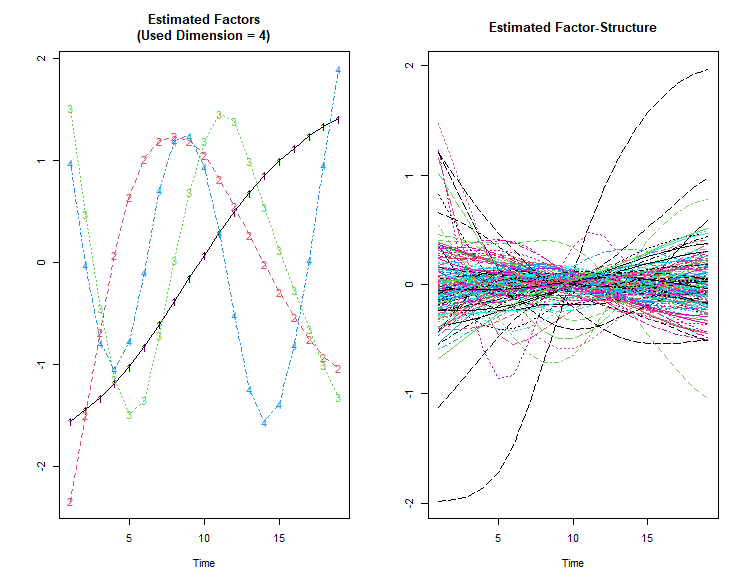
\includegraphics[width=\textwidth]{Images/factors_kss_reduced.png}
  \label{fig:image4}
\end{figure}


 


\begin{sidewaystable}
\caption{Effect of Democracy on GDP per capita \\
(\ac{KSS} method, Bootstrap Regression Analysis)}\label{KSS_results_appendix}
    \label{tab:full_table}
    \small
    \centering
    \resizebox{\textwidth}{!}{%
        \begin{tabular}{cccccc}
            \hline
            & Democracy & Log GDP, first lag & Log GDP, second lag & Log GDP, third lag & Log GDP, fourth lag \\
            \hline 
            Original Estimate & -0.0017 & -0.1874 & -0.2240 & -0.1331 & -0.1155 \\
            Bias & 0.0007 & 0.0063 & -0.00003 & 0.0021 & -0.0015 \\
            Bootstrap Standard Error & 0.0109 & 0.2563 & 0.0841 & 0.0451 & 0.0243 \\
            Median & -0.0009 & -0.1475 & -0.2065 & -0.1224 & -0.1163 \\
            Normal 95\% CI & (-0.0238, 0.0190) & (-0.6960, 0.3085) & (-0.3888, -0.0591) & (-0.2236, -0.0468) & (-0.1617, -0.0664) \\
            Percentile 95\% CI & (-0.0227, 0.0209) & (-0.6811, 0.1767) & (-0.4004, -0.0998) & (-0.2292, -0.0638) & (-0.1665, -0.0712) \\
            BCa 95\% CI & (-0.0228, 0.0208) & (-0.7029, 0.1603) & (-0.4175, -0.1084) & (-0.2394, -0.0688) & (-0.1671, -0.0716) \\
            \hline
        \end{tabular}%
    }
\end{sidewaystable}

\begin{figure}[htb]
  \caption{Histogram and Density Plot of Bootstrap Regression Coefficients for Democracy \\
  (\ac{KSS} method)}
  \centering
  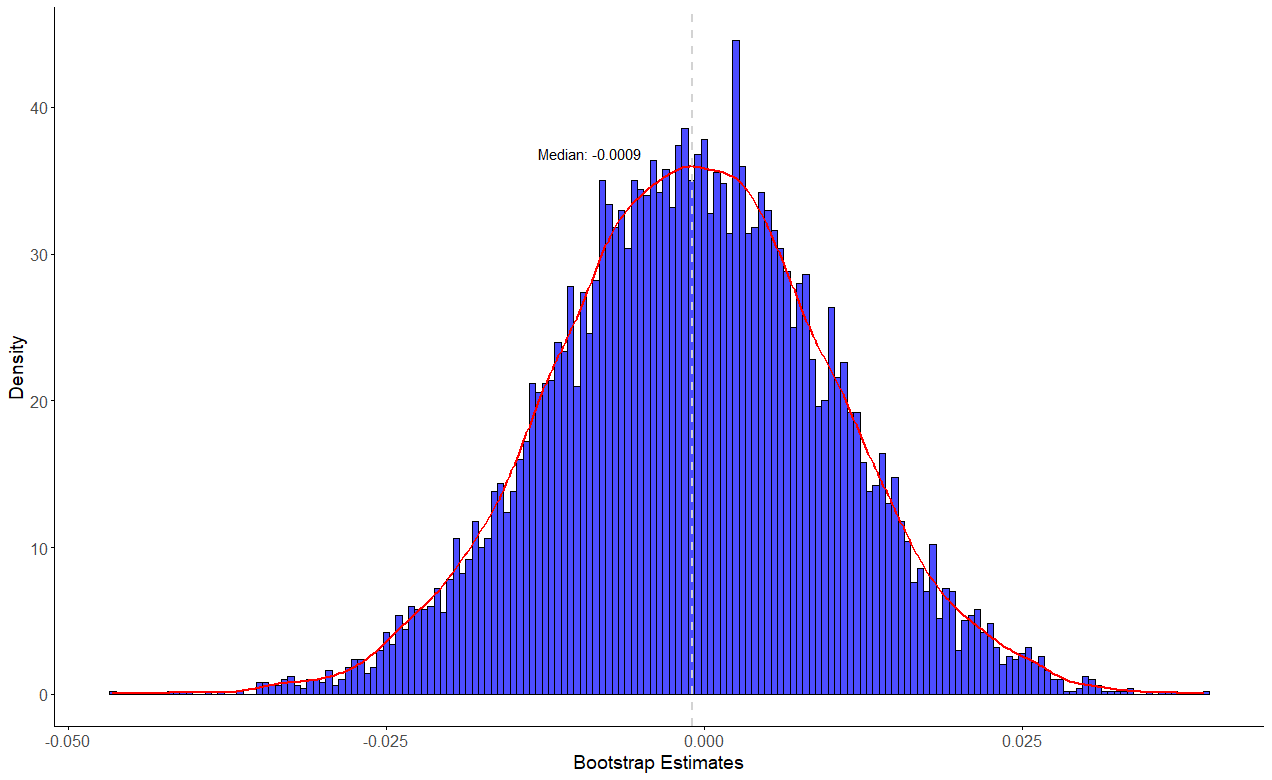
\includegraphics[width=\textwidth]{Images/kss_hist.png}
  \label{fig:image5}
\end{figure}


\subsection{Bootstrap-Regression Analysis via the \acs{Eup} method}\label{eup_apendix}

\begin{sidewaystable}
\caption{Effect of Democracy on GDP per capita growth \\
(\ac{Eup} method, Bootstrap-regression analysis)}
\label{eup_results_appendix}
\footnotesize
\centering
%\resizebox{\textwidth}{!}{%
\begin{tabular}{cccccc}
\hline
 & Democracy & $\Delta$ Log GDP, first lag &  $\Delta$ Log GDP, second lag & $\Delta$ Log GDP, third lag &  $\Delta$ Log GDP, fourth lag \\
\hline 
Original Estimate & -0.00201 & -0.57100 & -0.56100 & -0.42300 & -0.28300 \\
Bias & 0.00052 & 0.00062 & -0.00007 & -0.00004 & 0.00007 \\
Bootstrap Standard Error & 0.0048 & 0.0010 & 0.0011 & 0.0010 & 0.0007 \\
Median Estimate & -0.00152 & -0.57000 & -0.56100 & -0.42300 & -0.28300 \\
Normal 95\% CI & (-0.0120, 0.0069) & (-0.5736, -0.5697) & (-0.5630, -0.5589) & (-0.4248, -0.4211) & (-0.2845, -0.2817) \\
Percentile 95\% CI & (-0.0108, 0.0080) & (-0.5730, -0.5690) & (-0.5640, -0.5590) & (-0.4250, -0.4210) & (-0.2840, -0.2810) \\
BCa 95\% CI & (-0.0119, 0.0069) & (-0.5820, -0.5710) & (-0.5717, -0.5610) & (-0.4297, -0.4230) & (-0.2880, -0.2830) \\
\hline
\end{tabular}%
%}
\end{sidewaystable}
\end{appendix}
\clearpage







\end{document} 
